\documentclass{article}

\usepackage[utf8]{inputenc}
\usepackage{graphicx}
\usepackage{hyperref}
\usepackage{float} % Carga el paquete float
\usepackage{tikz}
\usepackage[margin=1in]{geometry}
\usepackage{listings} % Añade esto a tu preámbulo
\usepackage{xcolor} % Para colores

\setlength{\parskip}{1em} % Cambia 1em por el valor que prefieras

% Definición de colores estilo neón sobre fondo oscuro
\definecolor{backgroundcolor}{rgb}{0.1, 0.1, 0.1} % Fondo oscuro
\definecolor{commentcolor}{rgb}{0.5, 0.8, 0.5} % Comentarios en verde neón
\definecolor{keywordcolor}{rgb}{0.6, 0.6, 1.0} % Palabras clave en azul neón
\definecolor{stringcolor}{rgb}{0.9, 0.6, 0.2} % Cadenas en naranja neón
\definecolor{codecolor}{rgb}{0.7, 0.7, 0.7} % Código en gris claro

\lstdefinestyle{neonstyle}{
    backgroundcolor=\color{backgroundcolor},
    commentstyle=\color{commentcolor},
    keywordstyle=\color{keywordcolor},
    stringstyle=\color{stringcolor},
    basicstyle=\ttfamily\small\color{codecolor},
    breakatwhitespace=false,
    breaklines=true,
    captionpos=b,
    keepspaces=true,
    numbers=left,
    numbersep=5pt,
    numberstyle=\color{black}, % Números de línea en negro
    showspaces=false,
    showstringspaces=false,
    showtabs=false,
    tabsize=2,
    language=JavaScript
}

\lstset{style=neonstyle}

% Si quieres personalizar aún más, puedes definir el lenguaje JavaScript
\lstdefinelanguage{JavaScript}{
  keywords={break, case, catch, continue, debugger, default, delete, do, else,
    finally, for, function, if, in, instanceof, new, return, switch, this,
    throw, try, typeof, var, void, while, with},
  morecomment=[l]{//},
  morecomment=[s]{/*}{*/},
  morestring=[b]",
  morestring=[b]'
}

\usetikzlibrary{positioning}
\usepackage[left=0.6in, right=0.6in]{geometry}

\usepackage{fancyhdr}

\pagestyle{fancy}
\fancyhf{} % Limpia el encabezado y pie de página actuales

% Configura el encabezado
\fancyhead[L]{History of War} % Lado izquierdo
\fancyhead[C]{Pablo Seijo y David Carpintero} % Centro
\fancyhead[R]{\thepage} % Lado derecho

% Configura el pie de página
\fancyfoot[L]{USC} % Lado izquierdo
\fancyfoot[C]{Desarrollo de Aplicaciones Web} % Centro

\renewcommand{\headrulewidth}{0.4pt} % Línea decorativa debajo del encabezado
\renewcommand{\footrulewidth}{0pt} % Sin línea en el pie de página

\title{\textit{History of War}}
\author{Carpintero Díaz David, Seijo García Pablo}
\date{\today}

\begin{document}

\maketitle
\tableofcontents
\newpage

\section{History of War: Un camino por la historia}

Nuestra página web está dedicada a la historia bélica del mundo. La página web cuenta con diferentes secciones con información variada.
La sección más llamativa es un mapa interactivo que sirve como portal a las páginas de las batallas más significativas de todas las épocas. Este mapa permite explorar visualmente el desarrollo de conflictos, desde las antiguas guerras hasta los enfrentamientos contemporáneos, brindando una perspectiva única y global de la historia militar.

También cuenta con diversos apartados temáticos, donde se encuentra información detallada sobre guerras que han moldeado naciones enteras, batallas que han cambiado el curso de la historia y personajes legendarios cuyas acciones resonaron a lo largo del tiempo. Cada sección está cuidadosamente elaborada para ofrecer datos exhaustivos y análisis profundos, proporcionando un contexto completo para comprender el trasfondo y la importancia de cada acontecimiento.

Además contamos con una biblioteca, que cuenta con una selección de libros recomendados, cada uno abordando distintas épocas de la historia bélica con profundidad. Cada recomendación va acompañada de una breve pero informativa descripción, que te brindará una visión general del contenido y del enfoque particular del libro.

\newpage

\section{Inventario de Contenido}

Con el objetivo de establecer una estructura clara y organizada para el desarrollo de nuestra página web, hemos procedido a la elaboración de un inventario de contenido. Dicho inventario actúa como un esquema preliminar que facilitará la implementación final del sitio web.

\begin{figure}[H]
    \centering
    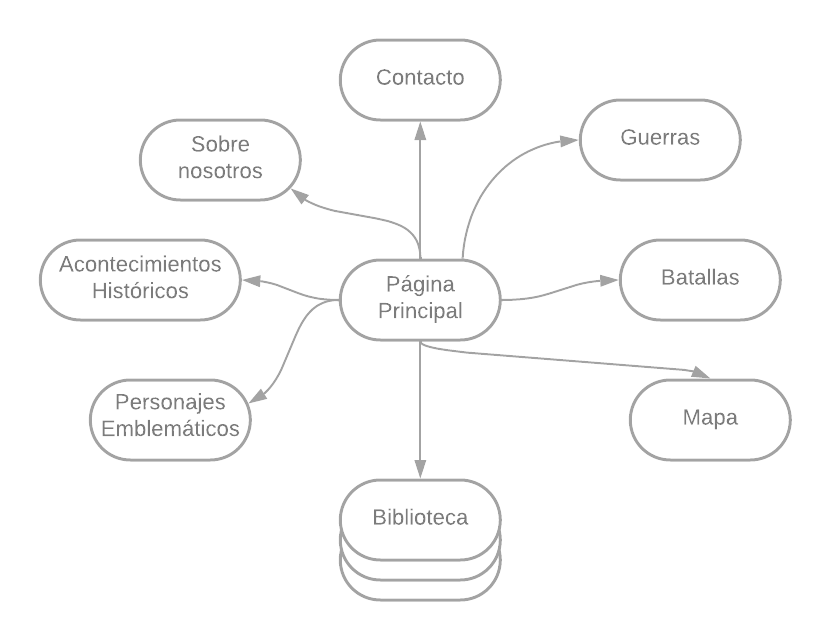
\includegraphics[width=0.6\textwidth]{Esquemas/InventarioContenido.png}
    \caption{Inventario de Contenido}
    \label{fig:mi_imagen}
\end{figure}

Nuestra plataforma se articula en diversas secciones, cada una con un propósito específico y contenido diferenciado. De particular relevancia es la sección denominada "Biblioteca", la cual albergará una selección cuidadosamente curada de libros recomendados. Asimismo, destacamos la inclusión de un mapa interactivo, diseñado para guiar a los usuarios a través de diversos episodios históricos, permitiéndoles explorar las distintas batallas que han marcado el curso del tiempo. Adicionalmente, la sección dedicada a las guerras ofrecerá una visión exhaustiva sobre los múltiples conflictos bélicos que han tenido lugar a lo largo de la historia, proporcionando información detallada y contextos relevantes.

\newpage

\section{Arquitectura de la Información}

Basándonos en el esquema preliminar previamente delineado, procedemos a desarrollar la arquitectura de la información. Este proceso nos facilitará la organización de las ideas iniciales en una estructura jerárquica, la cual establecerá la profundidad y el alcance de cada sección dentro de nuestra página web.

\begin{figure}[H]
    \centering
    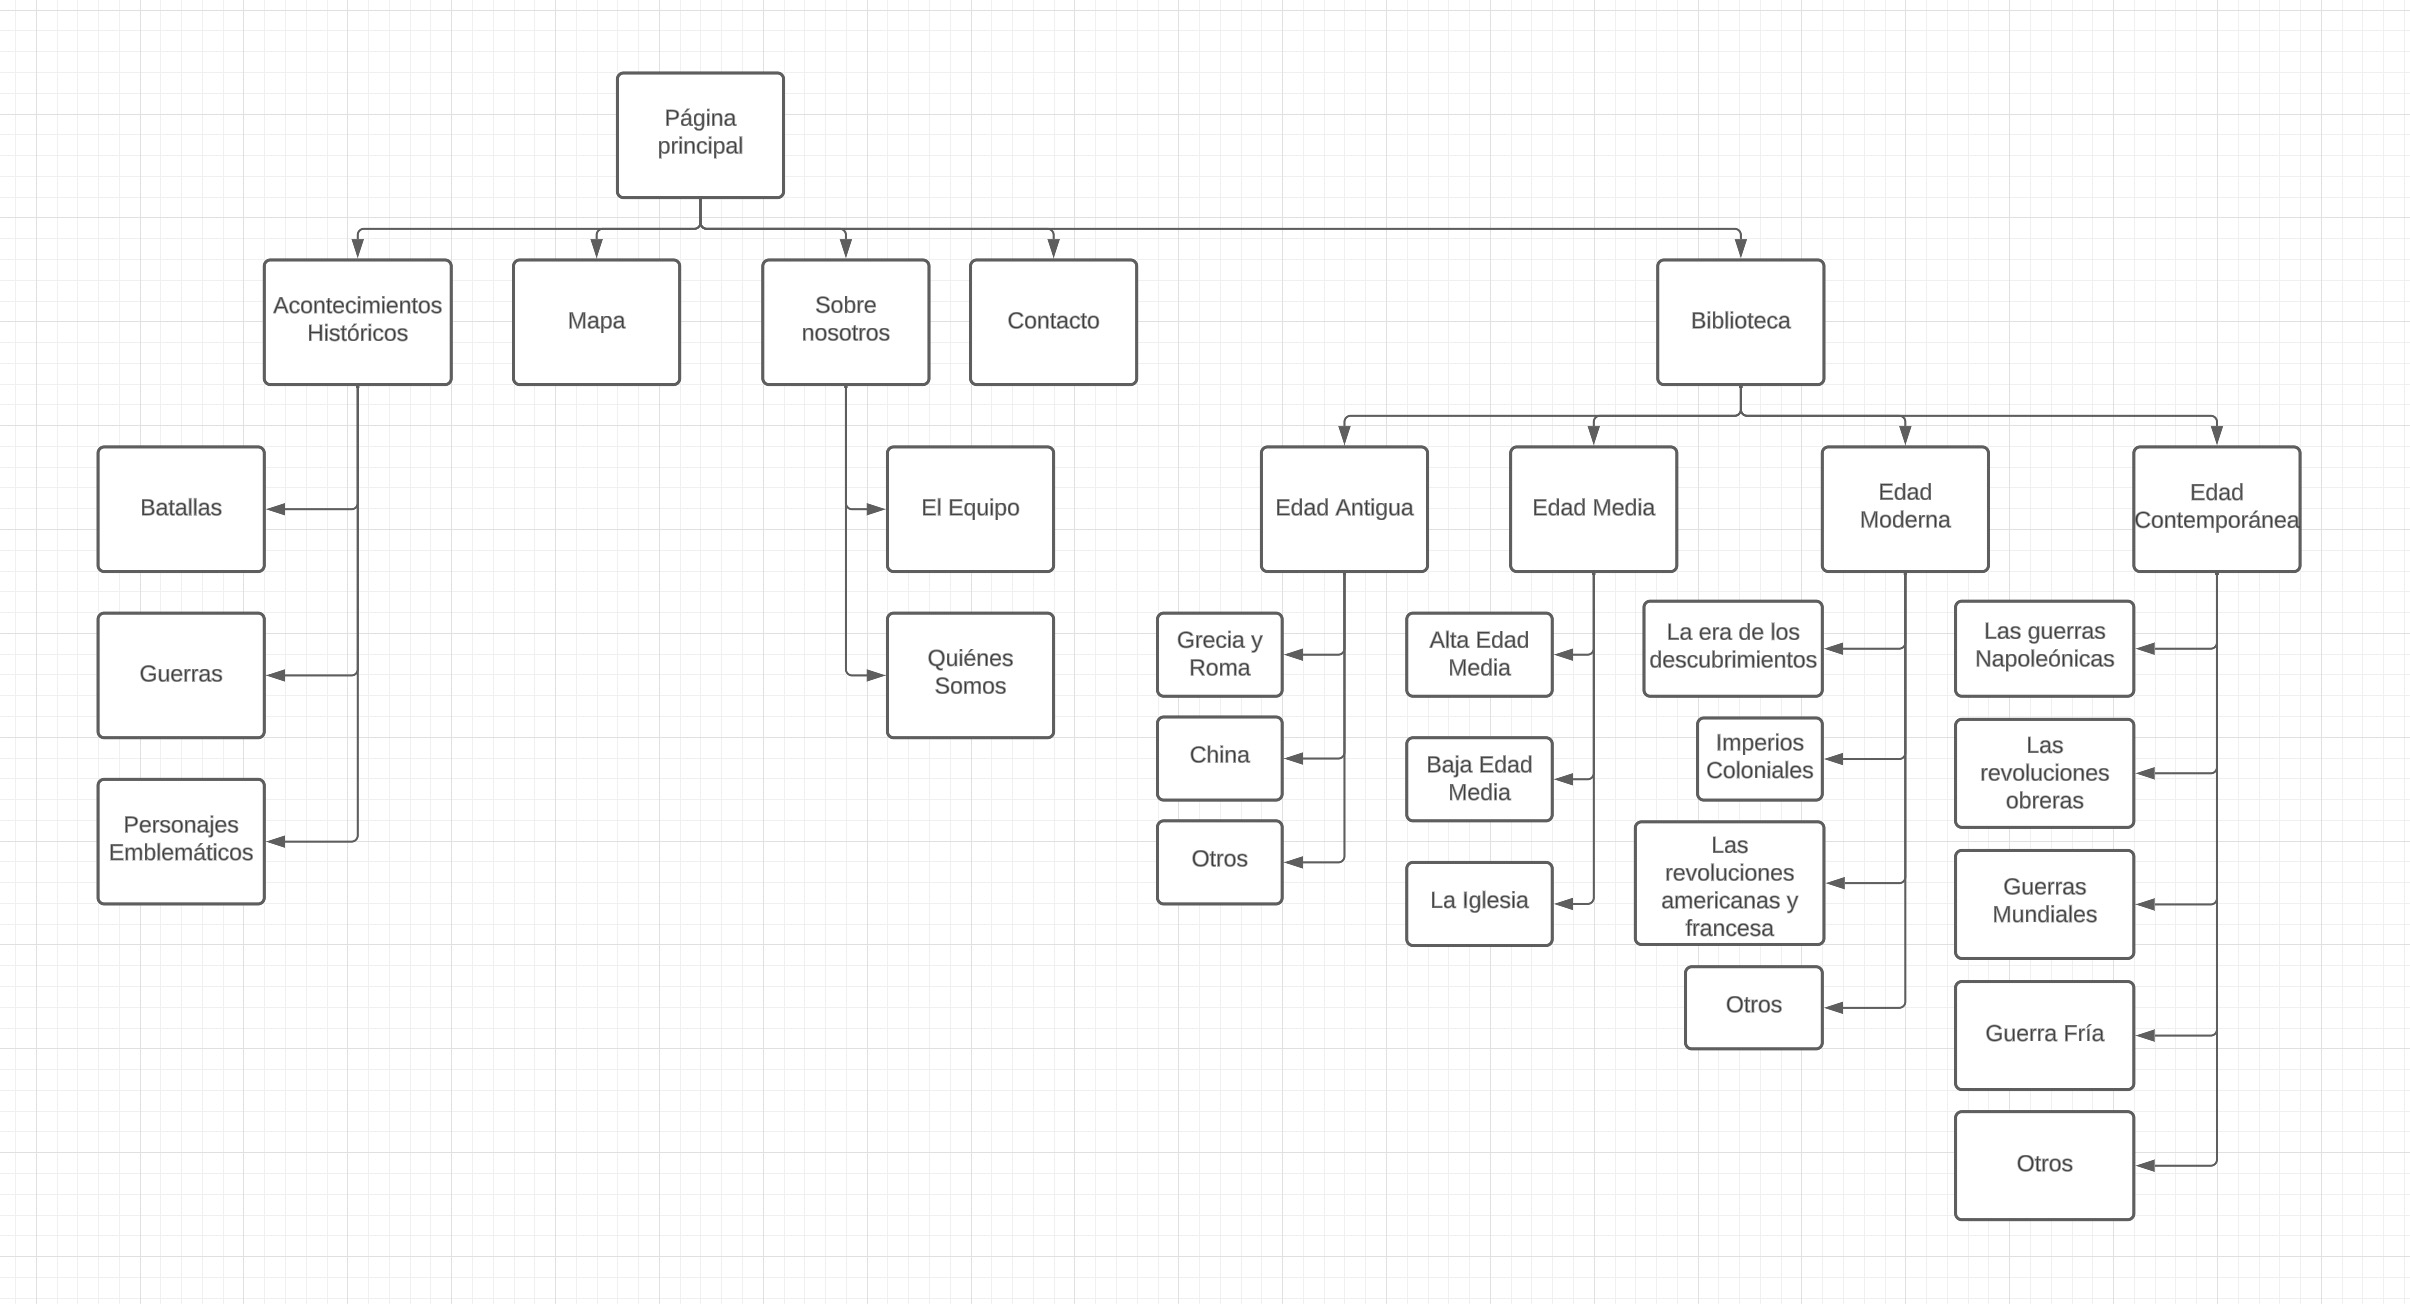
\includegraphics[width=1\textwidth]{Esquemas/Arquitectura de Informacion.jpg}
    \caption{Arquitectura de la Información}
    \label{fig:mi_imagen}
\end{figure}

Dentro de esta arquitectura, la sección más amplia corresponde a la biblioteca. Esta área está meticulosamente segmentada en diversas subsecciones que reflejan las distintas eras históricas, abarcando desde la Edad Antigua, iniciando en el año 3000 a.C., hasta la contemporaneidad. Esta organización no solo facilita la navegación sino que también enriquece la experiencia educativa del usuario al proporcionar un contexto histórico claro y bien definido.

Adicionalmente, cabe resaltar la sección denominada "Acontecimientos Históricos", la cual funciona como categoría principal para temas relacionados con guerras, batallas y figuras históricas destacadas. Esta categorización permite una exploración temática coherente y detallada de los eventos que han moldeado la historia humana.

En conjunto, la arquitectura de la información diseñada busca optimizar la usabilidad y accesibilidad del sitio web, asegurando que los usuarios puedan navegar de manera intuitiva y obtener información de forma eficiente.

\newpage

\section{Casos de Uso Típicos}

Tras definir la estructura de nuestro sitio web, presentaremos los casos de uso comunes, los cuales mostrarán las acciones que los usuarios pueden realizar al visitar nuestra página.

Esta parte es esencial para entender cómo los visitantes interactúan con el sitio, desde explorar las diferentes secciones hasta acceder a contenidos específicos. El objetivo es proporcionar una visión clara de lo que se espera que los usuarios hagan y cómo pueden aprovechar al máximo los recursos disponibles en la web.

\begin{figure}[H]
    \centering
    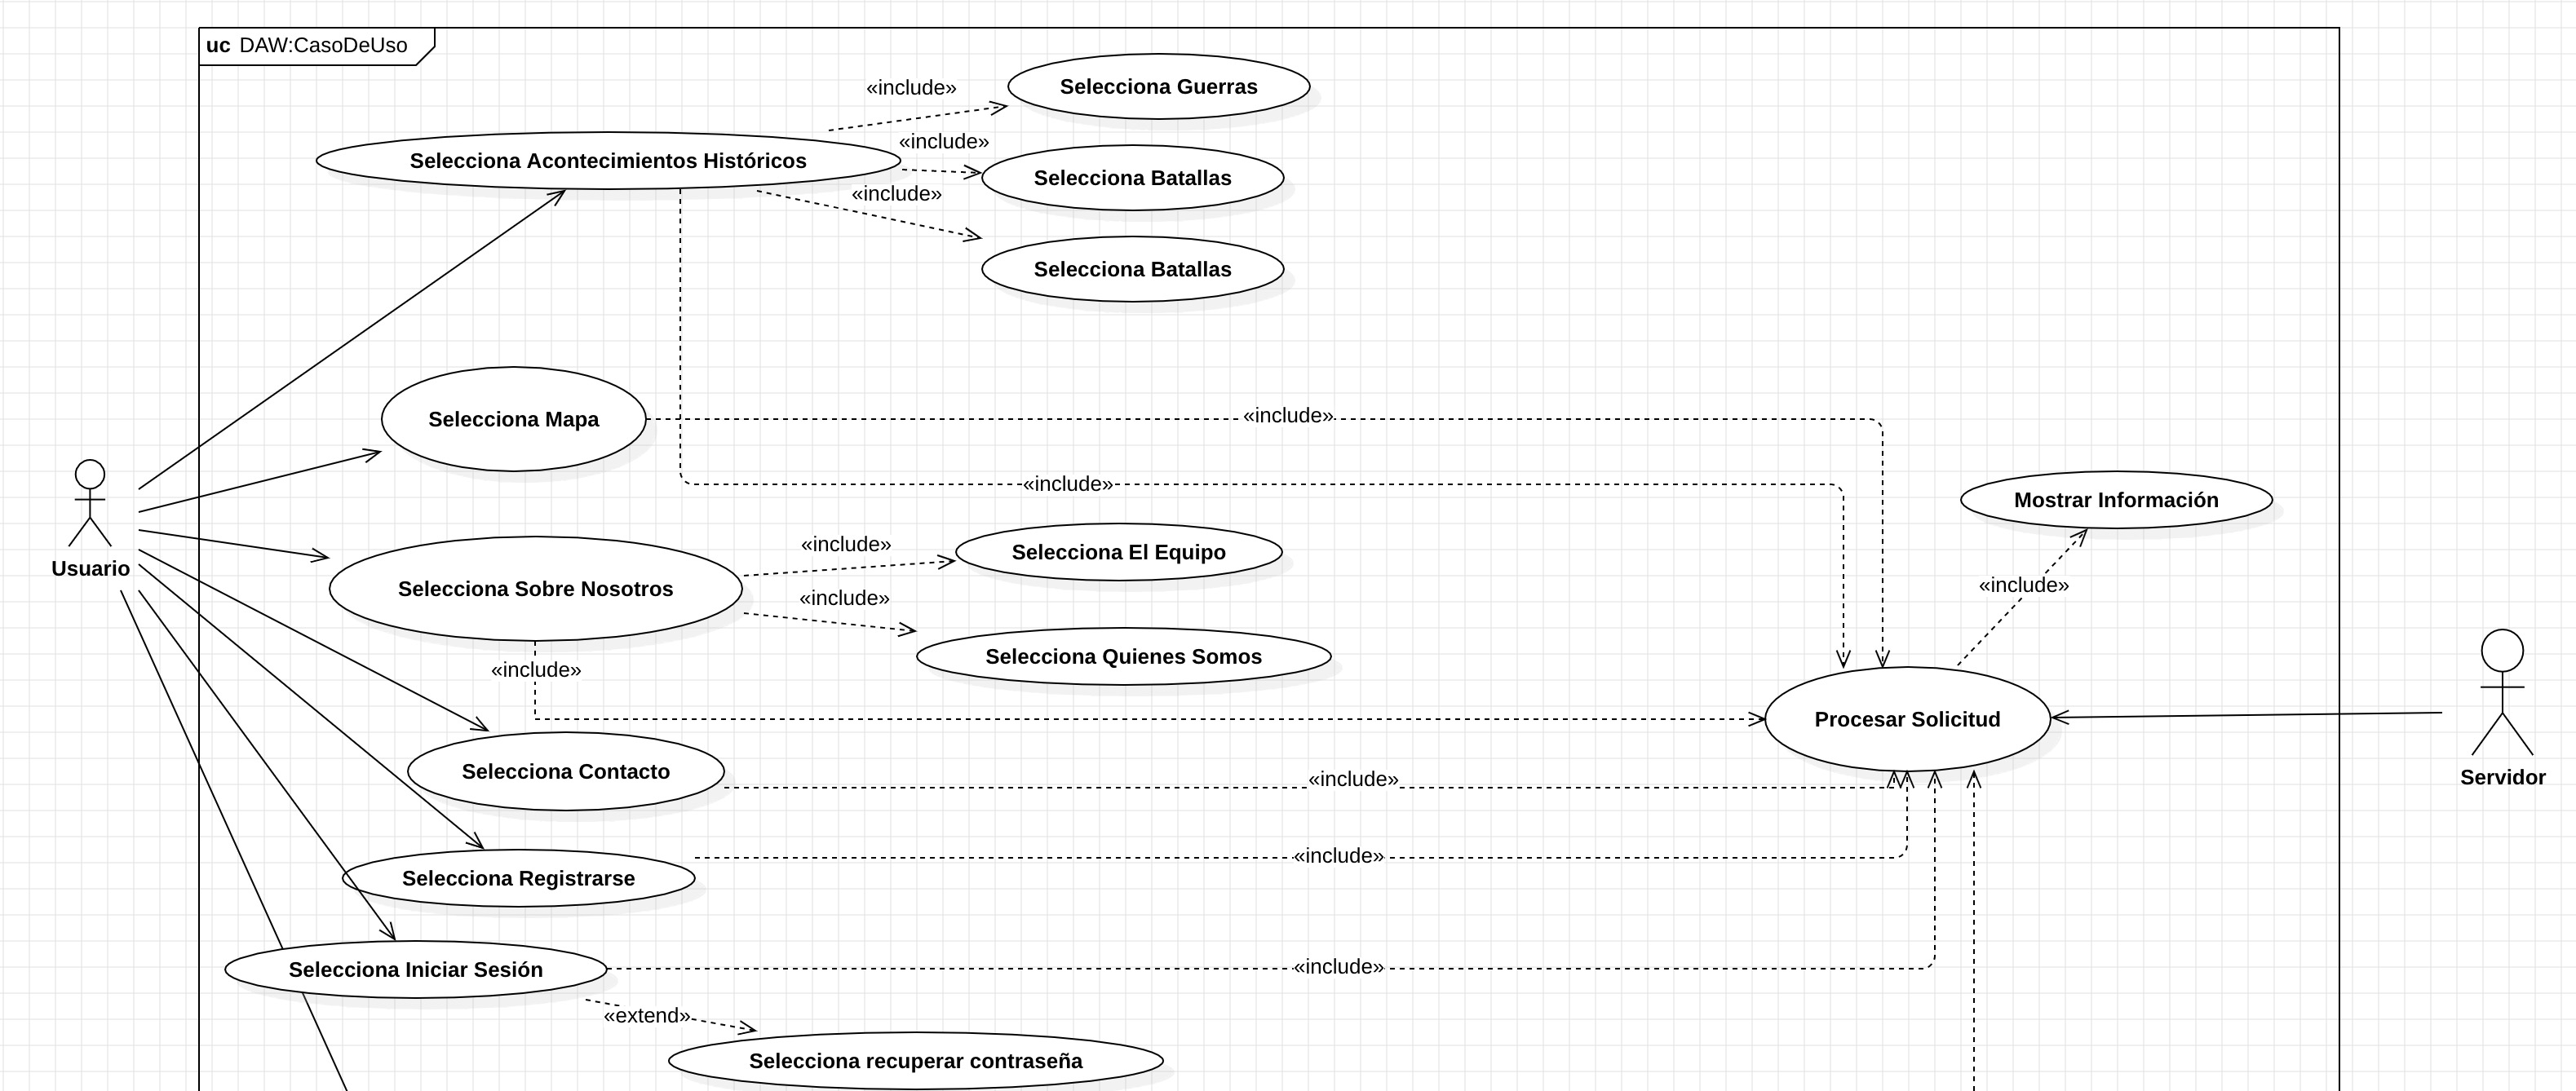
\includegraphics[width=1\textwidth]{Esquemas/CasosDeUsoSegmentado(1).jpg}
    \caption{Casos de Uso Típicos (1)}
    \label{fig:mi_imagen}
\end{figure}

\begin{figure}[H]
    \centering
    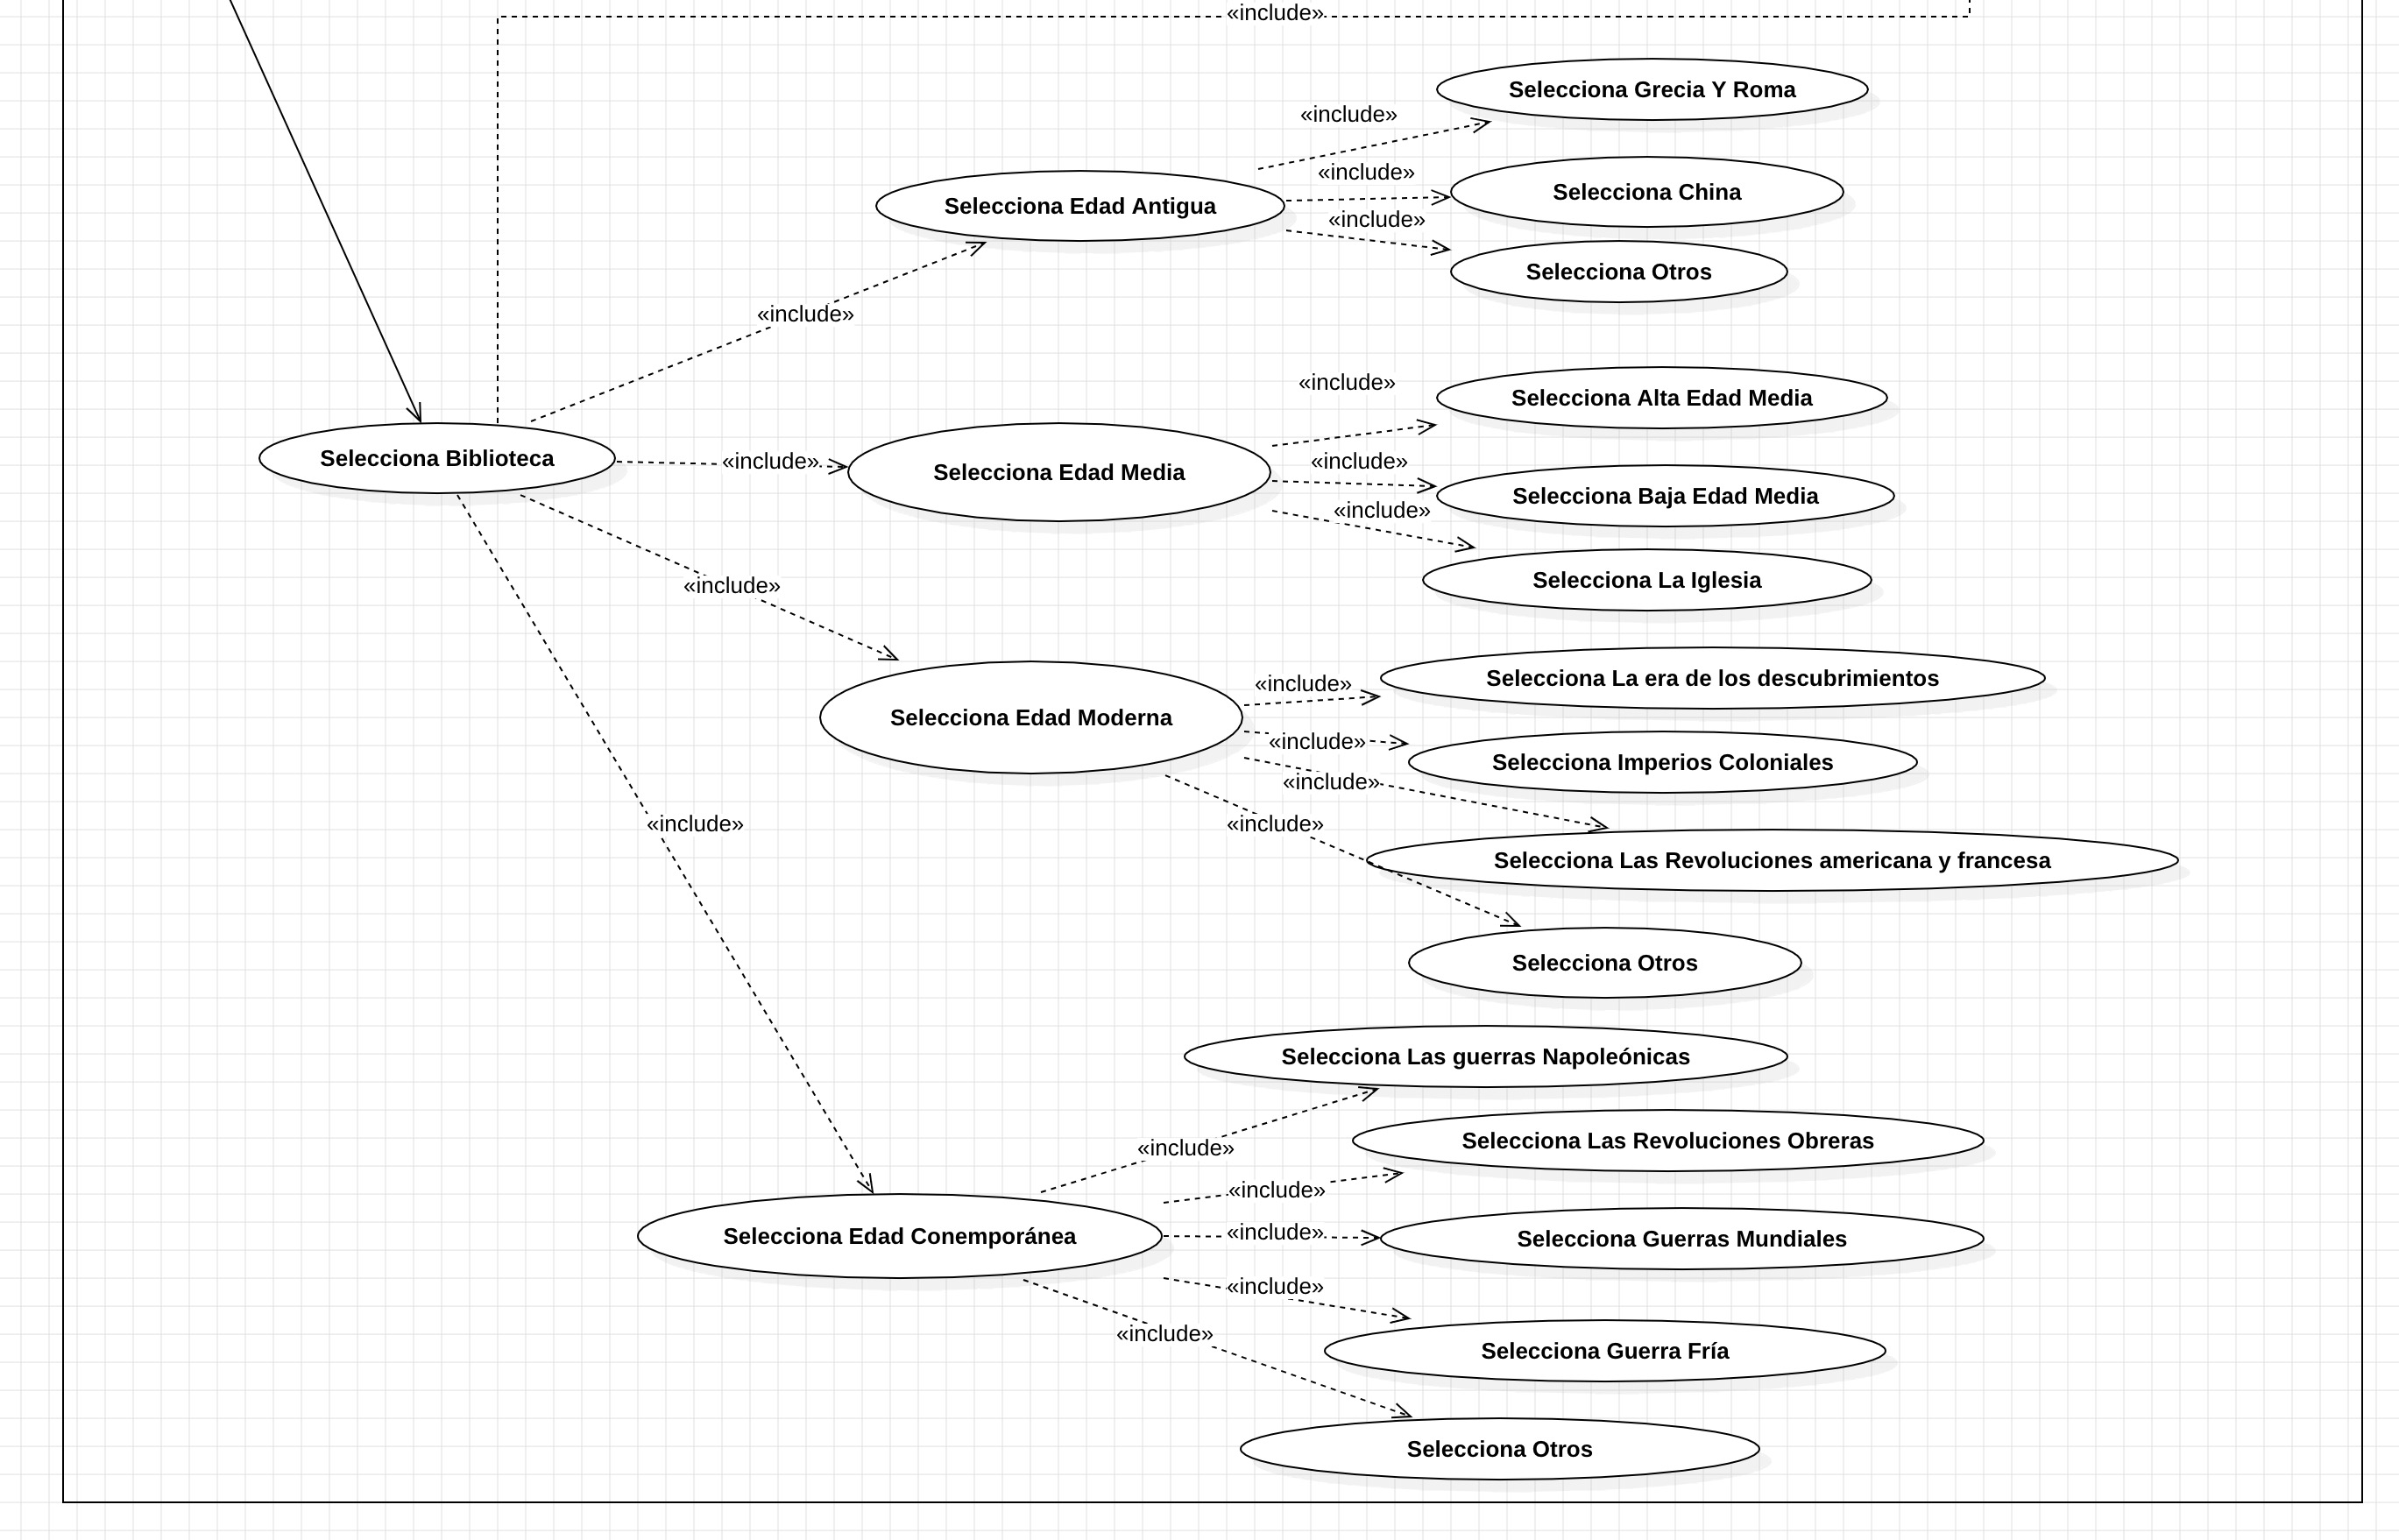
\includegraphics[width=1\textwidth]{Esquemas/CasosDeUsoSegamentado(2).jpg}
    \caption{Casos de Uso Típicos (2)}
    \label{fig:mi_imagen}
\end{figure}

\newpage

\section{Mapa de Navegación}

El mapa de navegación es un elemento clave en el diseño de nuestro sitio web, que actúa como una guía visual para estructurar y presentar la forma en que las distintas páginas y secciones están interconectadas. Este mapa facilita la comprensión de la organización del sitio, permitiendo a los usuarios y desarrolladores visualizar la jerarquía de la información y las rutas de acceso disponibles para navegar por el contenido. Al ofrecer una representación clara de cómo se organizan y relacionan los distintos componentes del sitio, el mapa de navegación mejora la usabilidad y la experiencia de usuario, asegurando que la información sea accesible y fácil de encontrar.

\begin{figure}[H]
    \centering
    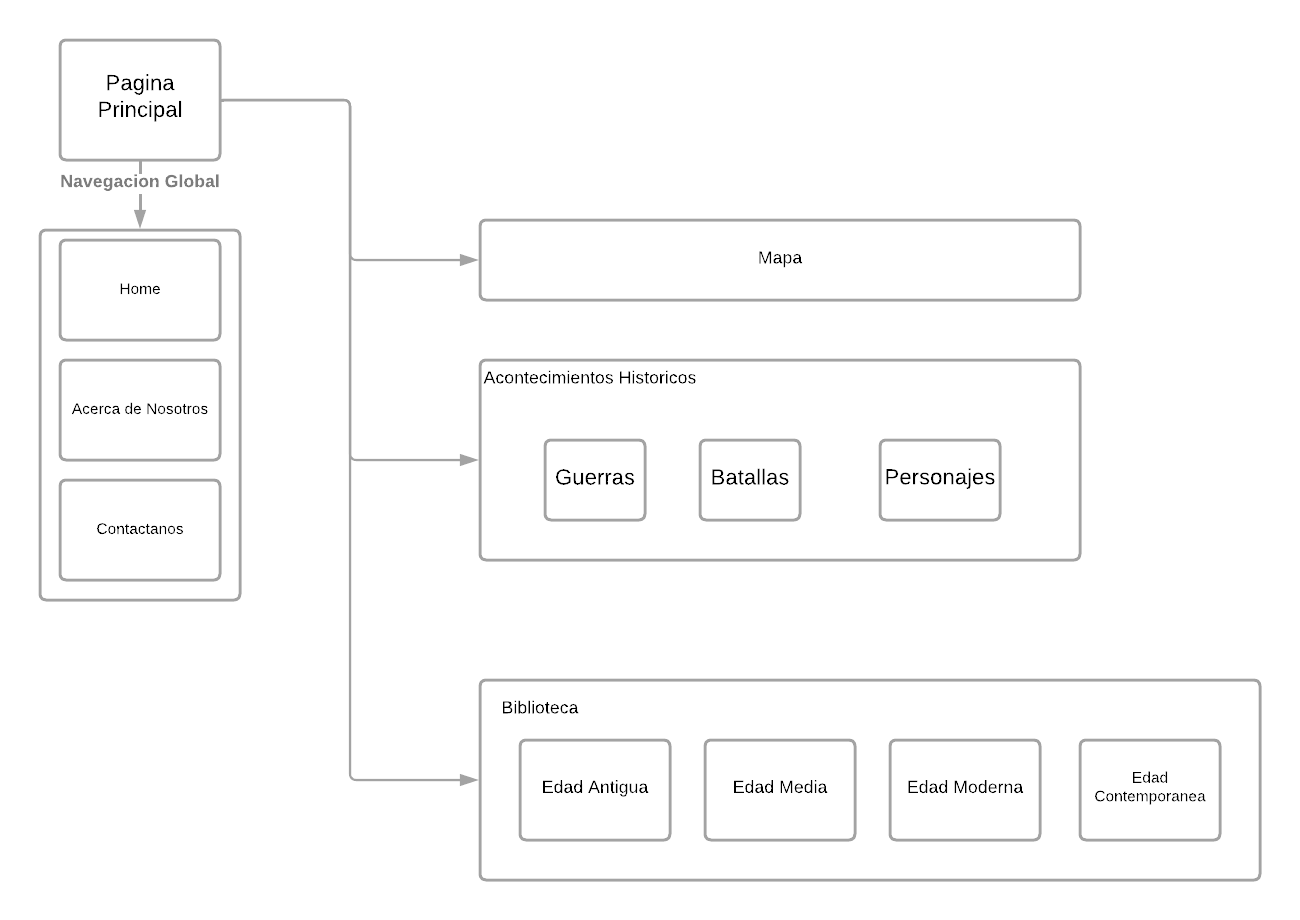
\includegraphics[width=1\textwidth]{Esquemas/MapawebFinal.png}
    \caption{Mapa de Navegación}
    \label{fig:mi_imagen}
\end{figure}

\newpage

\section{Interfaces}

\subsection{Manual (Boceto Manual)}

Se trata de un boceto manual de como nos imaginamos la página web, de tal manera que basaremos la evolución de la página basándonos en este concepto primigenio de las páginas.

\begin{figure}[H]
    \centering
    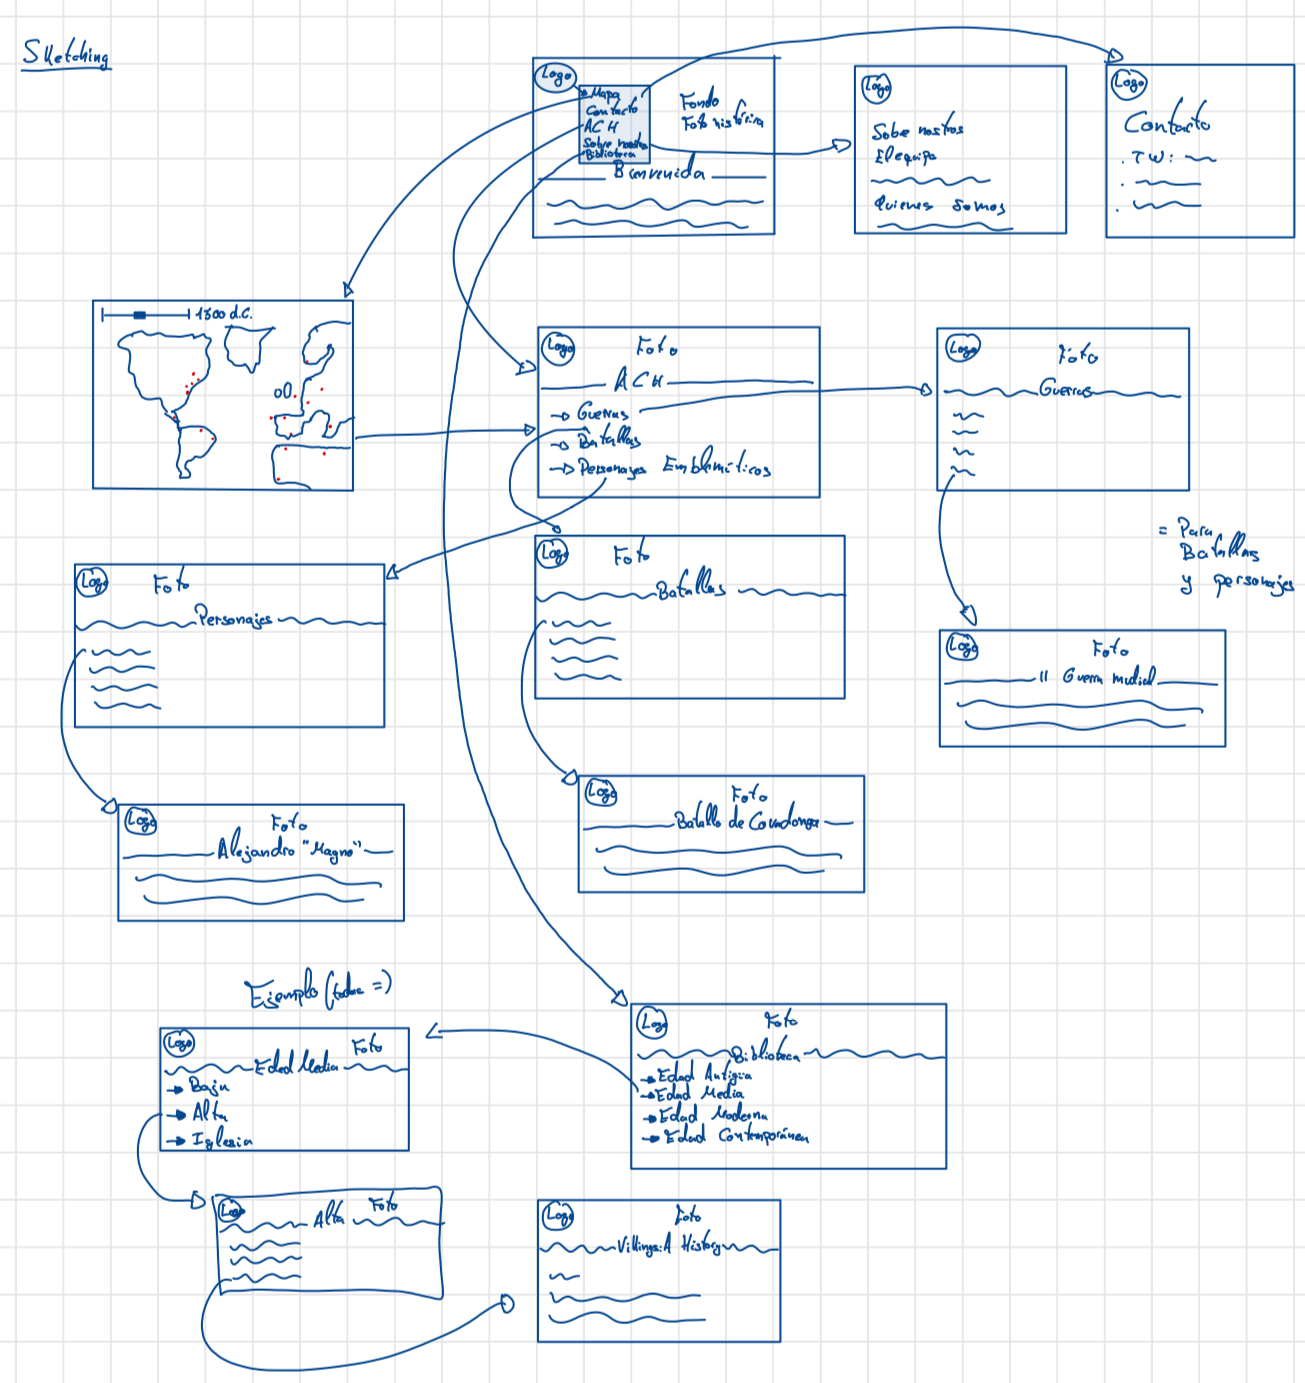
\includegraphics[width=1\textwidth]{Esquemas/Sketch.PNG}
    \caption{Boceto Manual}
    \label{fig:mi_imagen}
\end{figure}

\newpage

\subsection{Wireframes}

Los wireframes constituyen un conjunto de esquemas visuales que representan de forma preliminar el diseño y la estructura de nuestra página web. Estos bocetos iniciales son fundamentales para conceptualizar la disposición de los elementos en las páginas, sirviendo como base para el desarrollo y refinamiento posterior del sitio. A través de estos wireframes, establecemos un marco de referencia que guiará las fases subsiguientes del diseño, asegurando que la visión original se mantenga coherente a lo largo del proceso de desarrollo.

\begin{figure}[H]
    \centering
    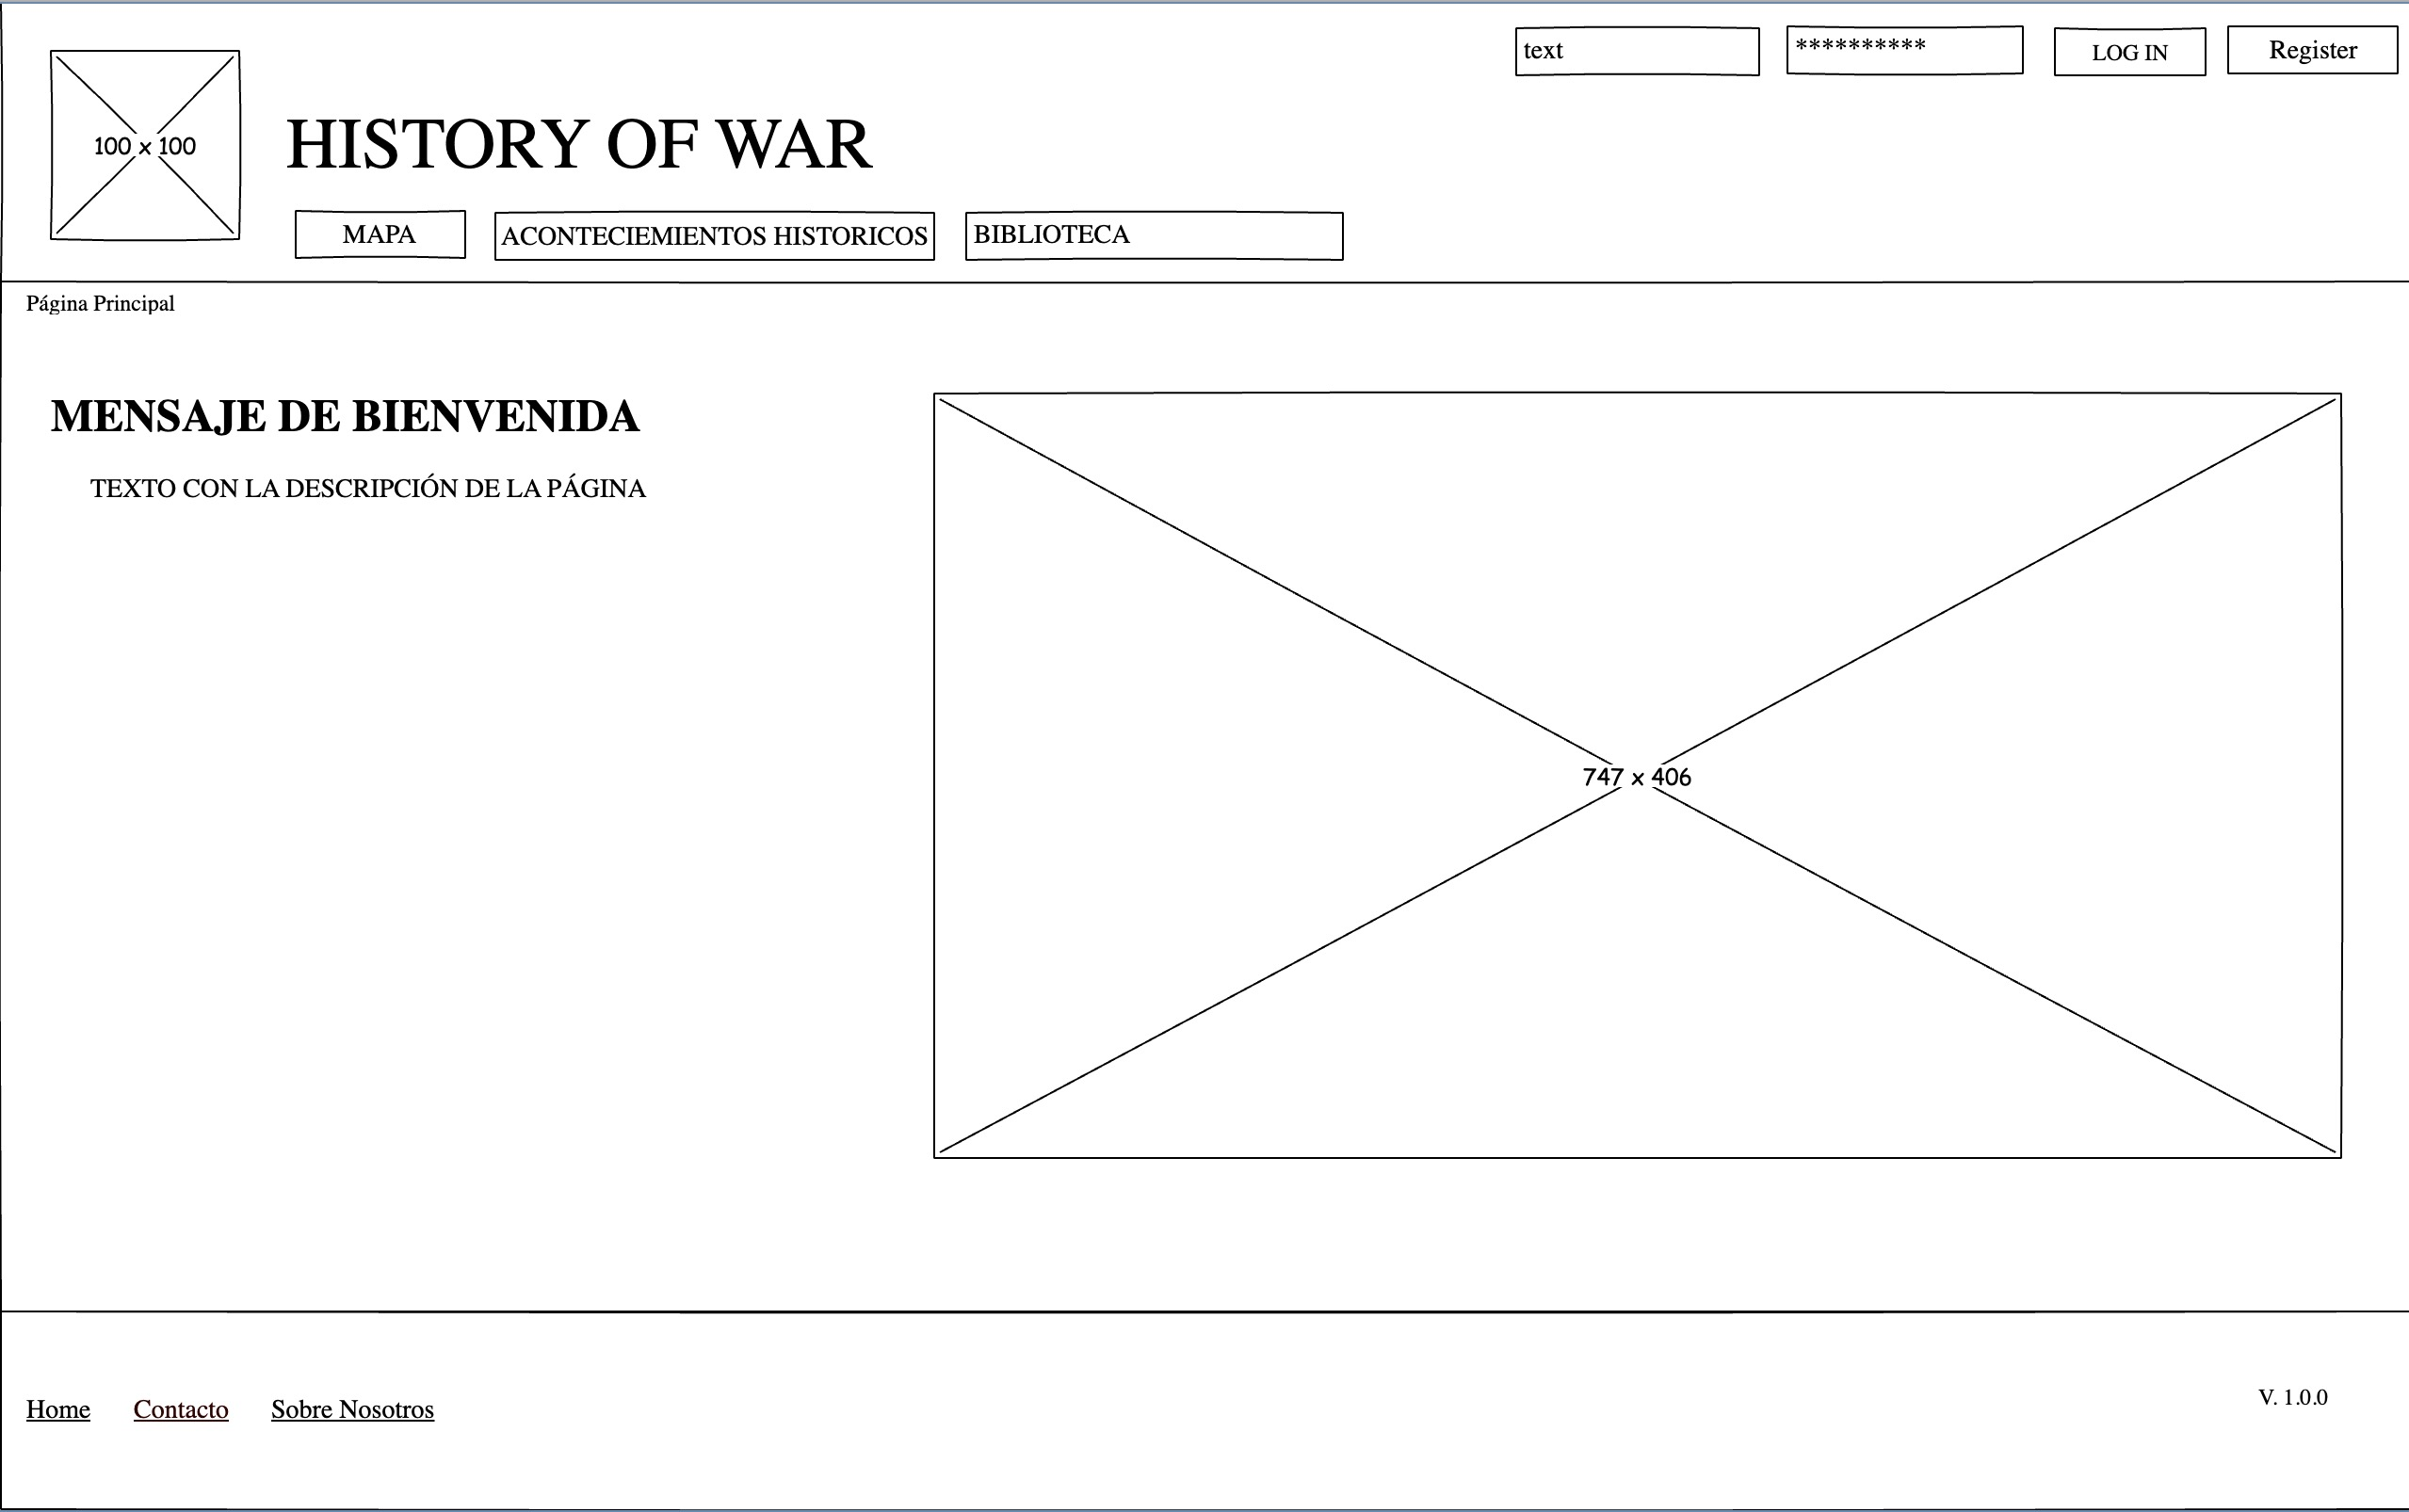
\includegraphics[width=1\textwidth]{Wireframes/PaginaPrincipal.jpg}
    \caption{Página Principal}
    \label{fig:mi_imagen}
\end{figure}

\begin{figure}[H]
    \centering
    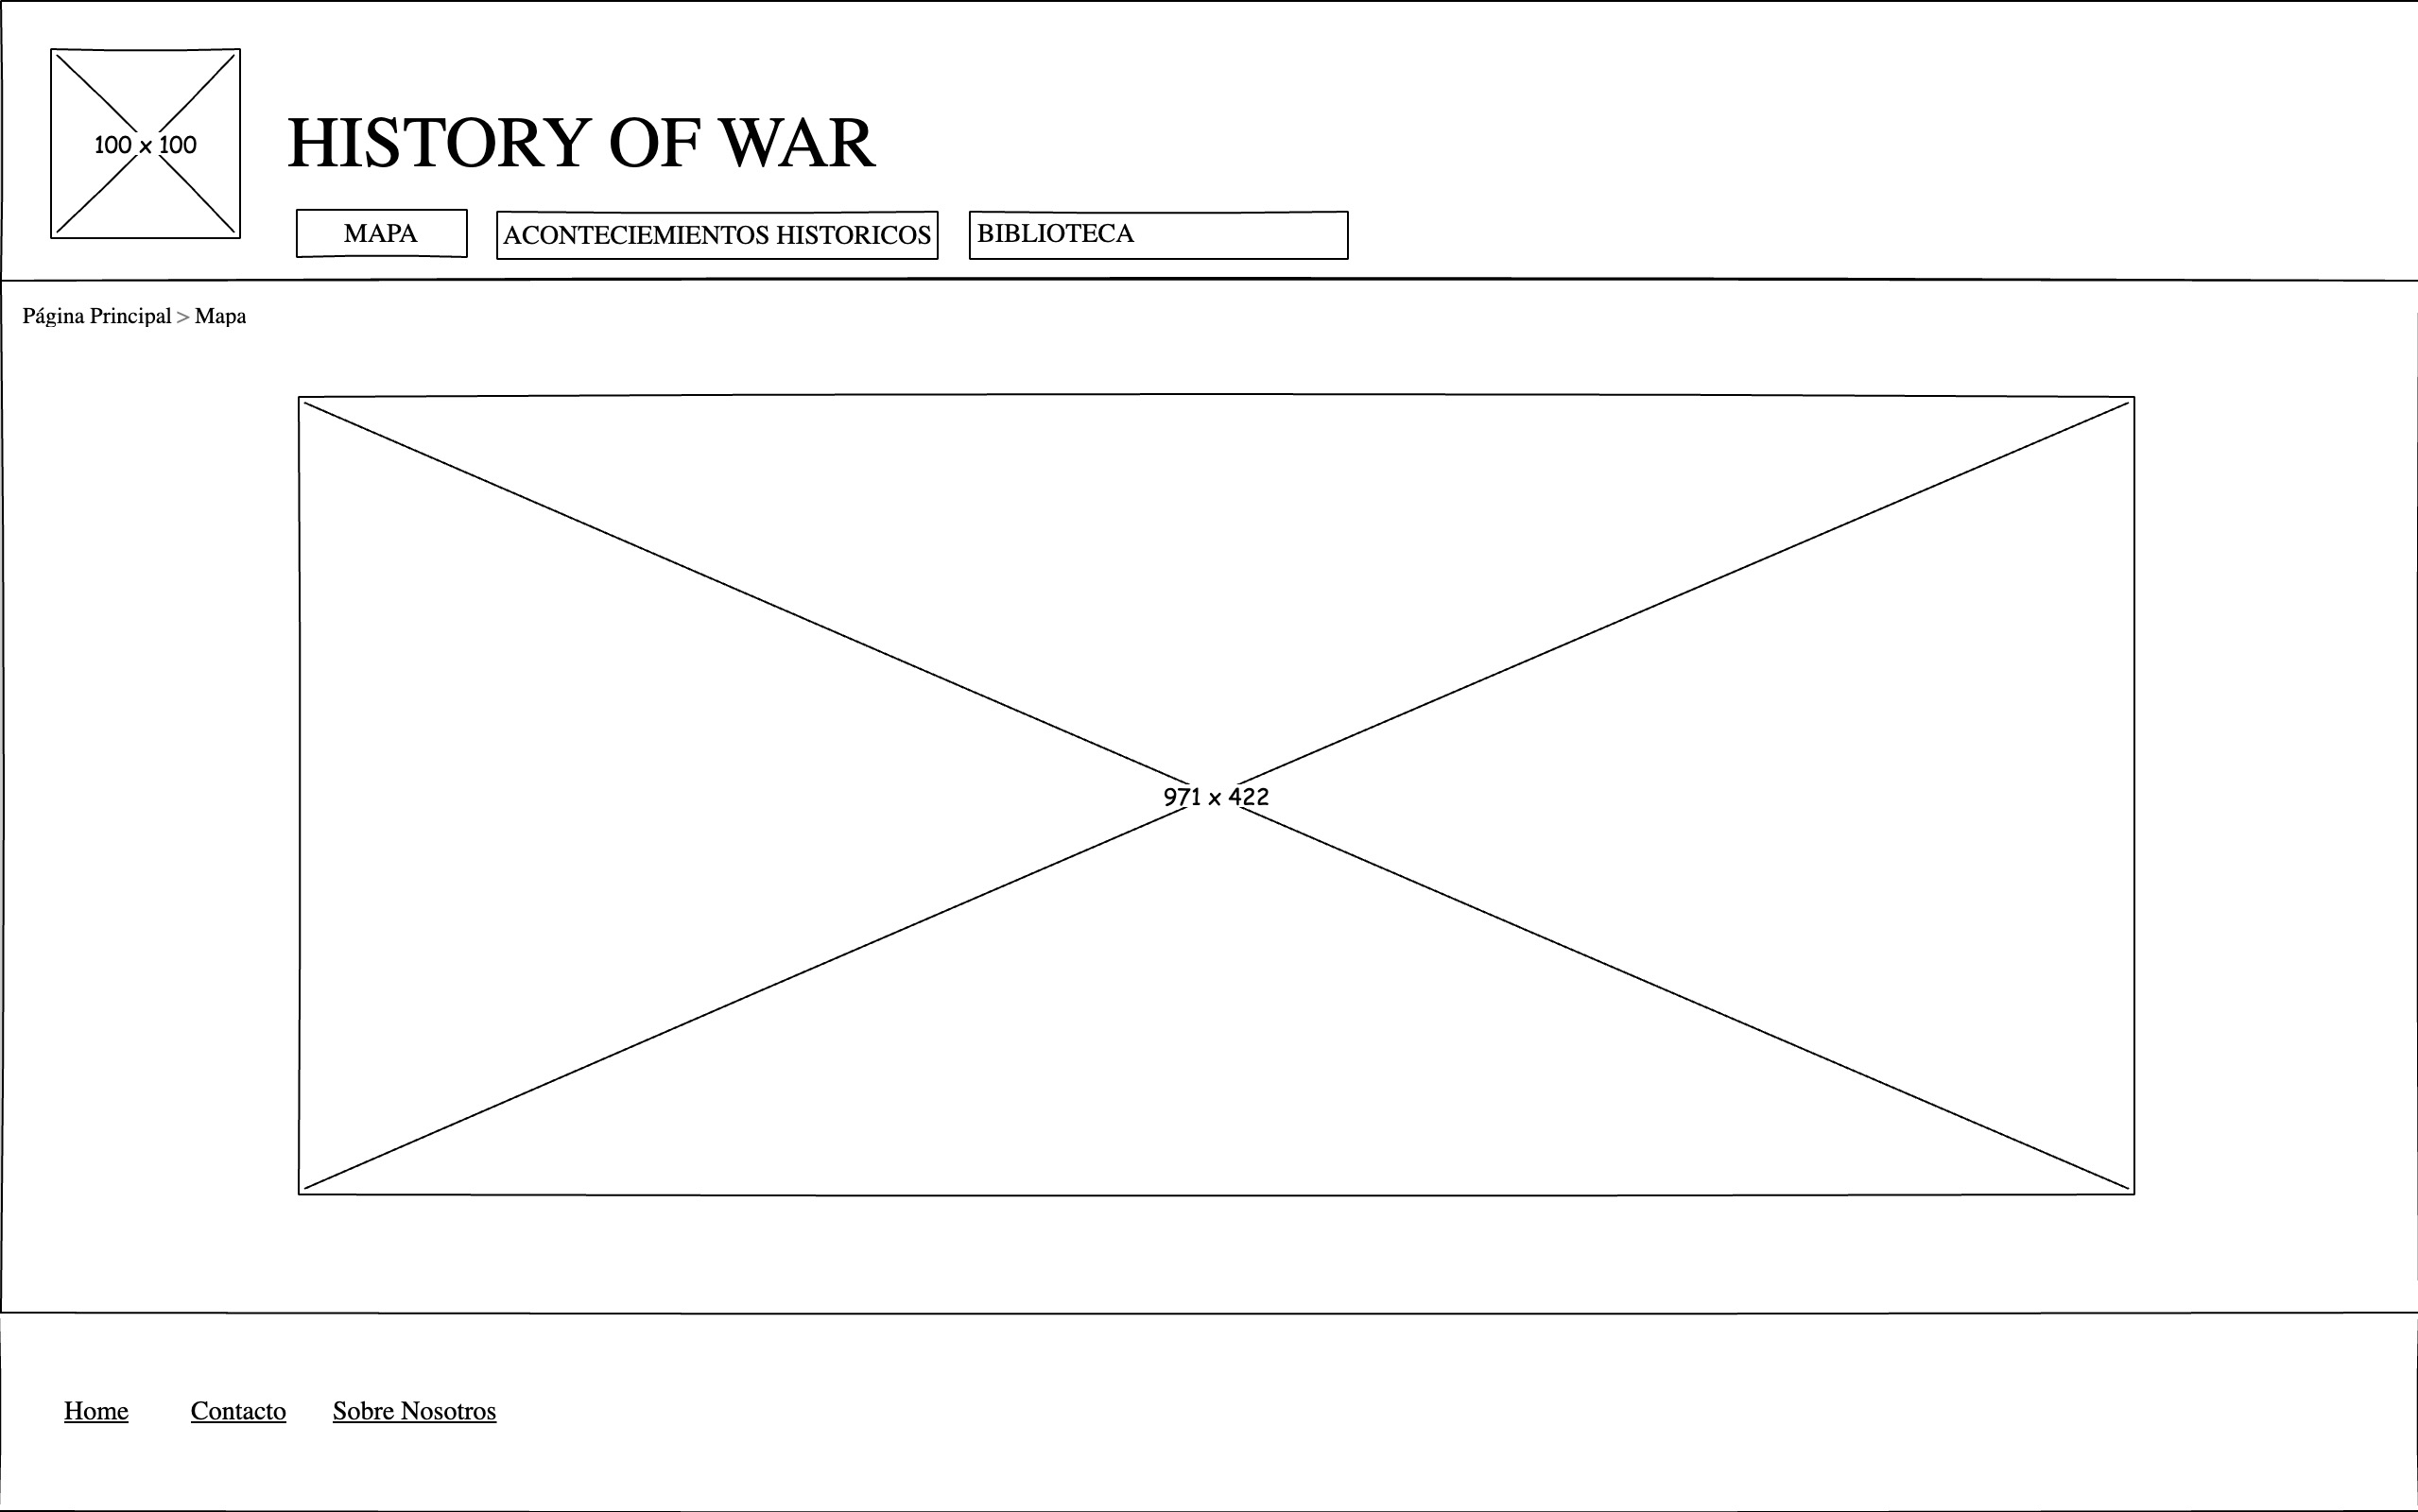
\includegraphics[width=1\textwidth]{Wireframes/Mapa.jpg}
    \caption{Mapa}
    \label{fig:mi_imagen}
\end{figure}

\begin{figure}[H]
    \centering
    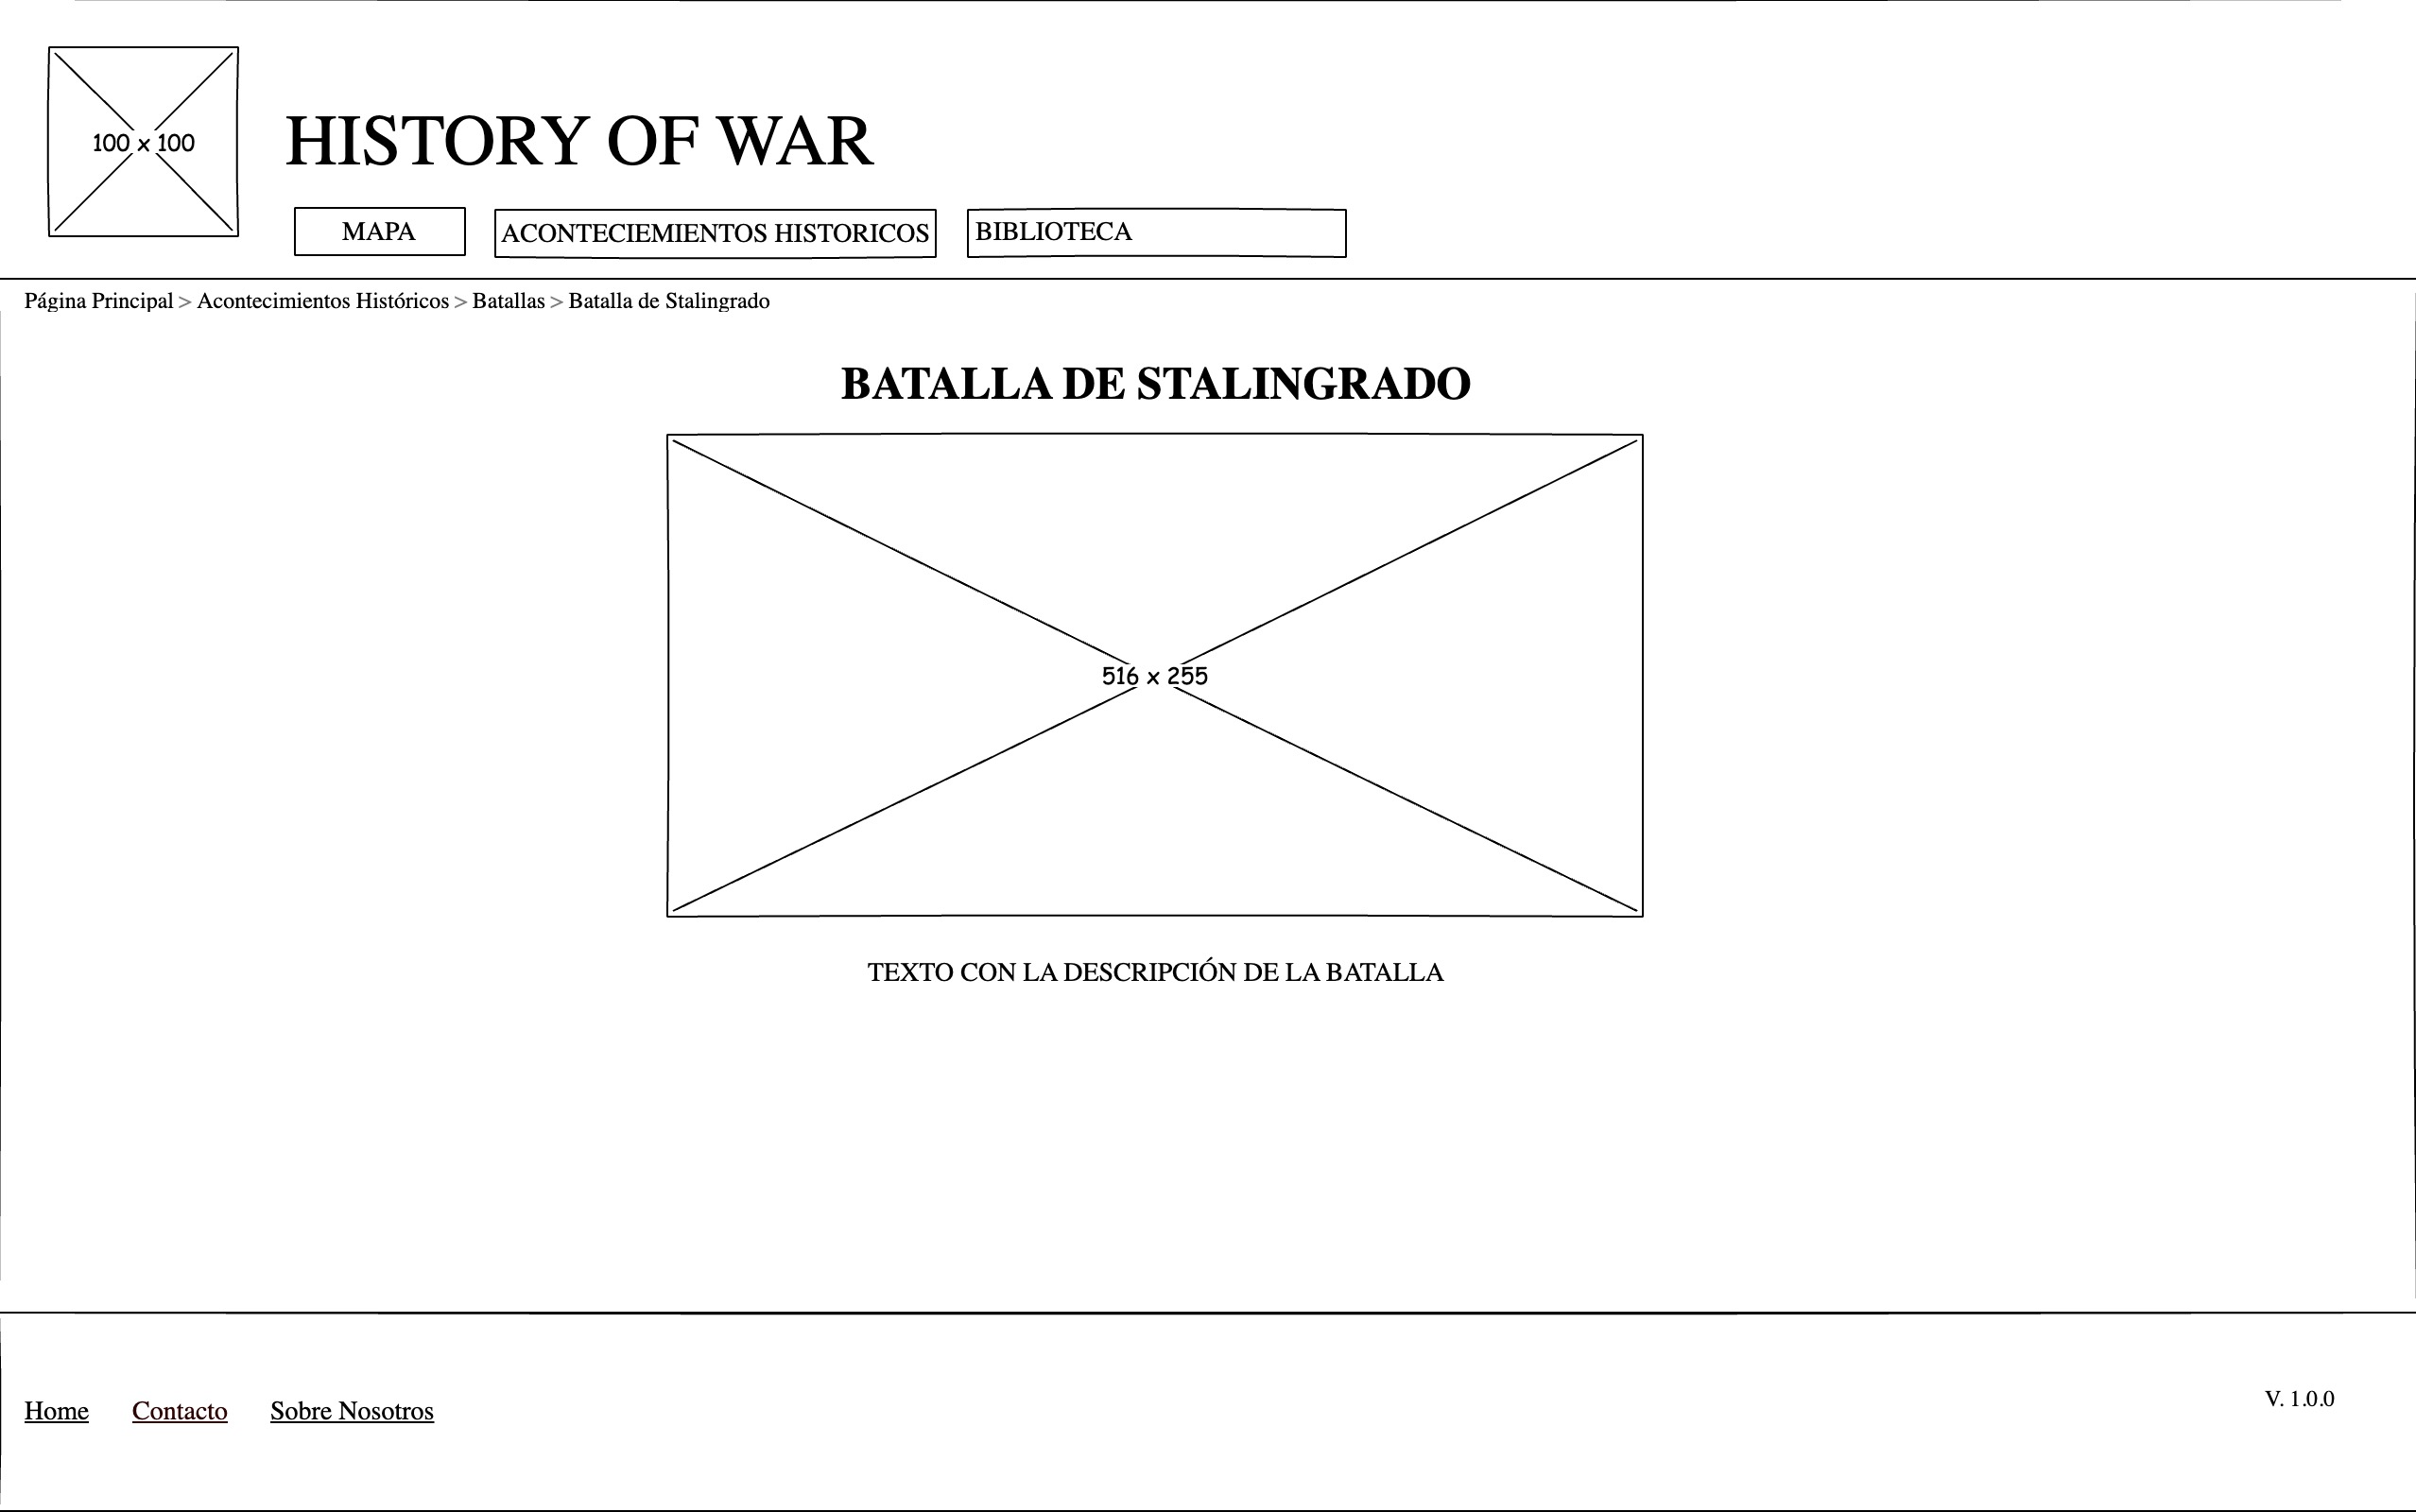
\includegraphics[width=1\textwidth]{Wireframes/EjemploBatalla.jpg}
    \caption{Ejemplo Batalla}
    \label{fig:mi_imagen}
\end{figure}

\begin{figure}[H]
    \centering
    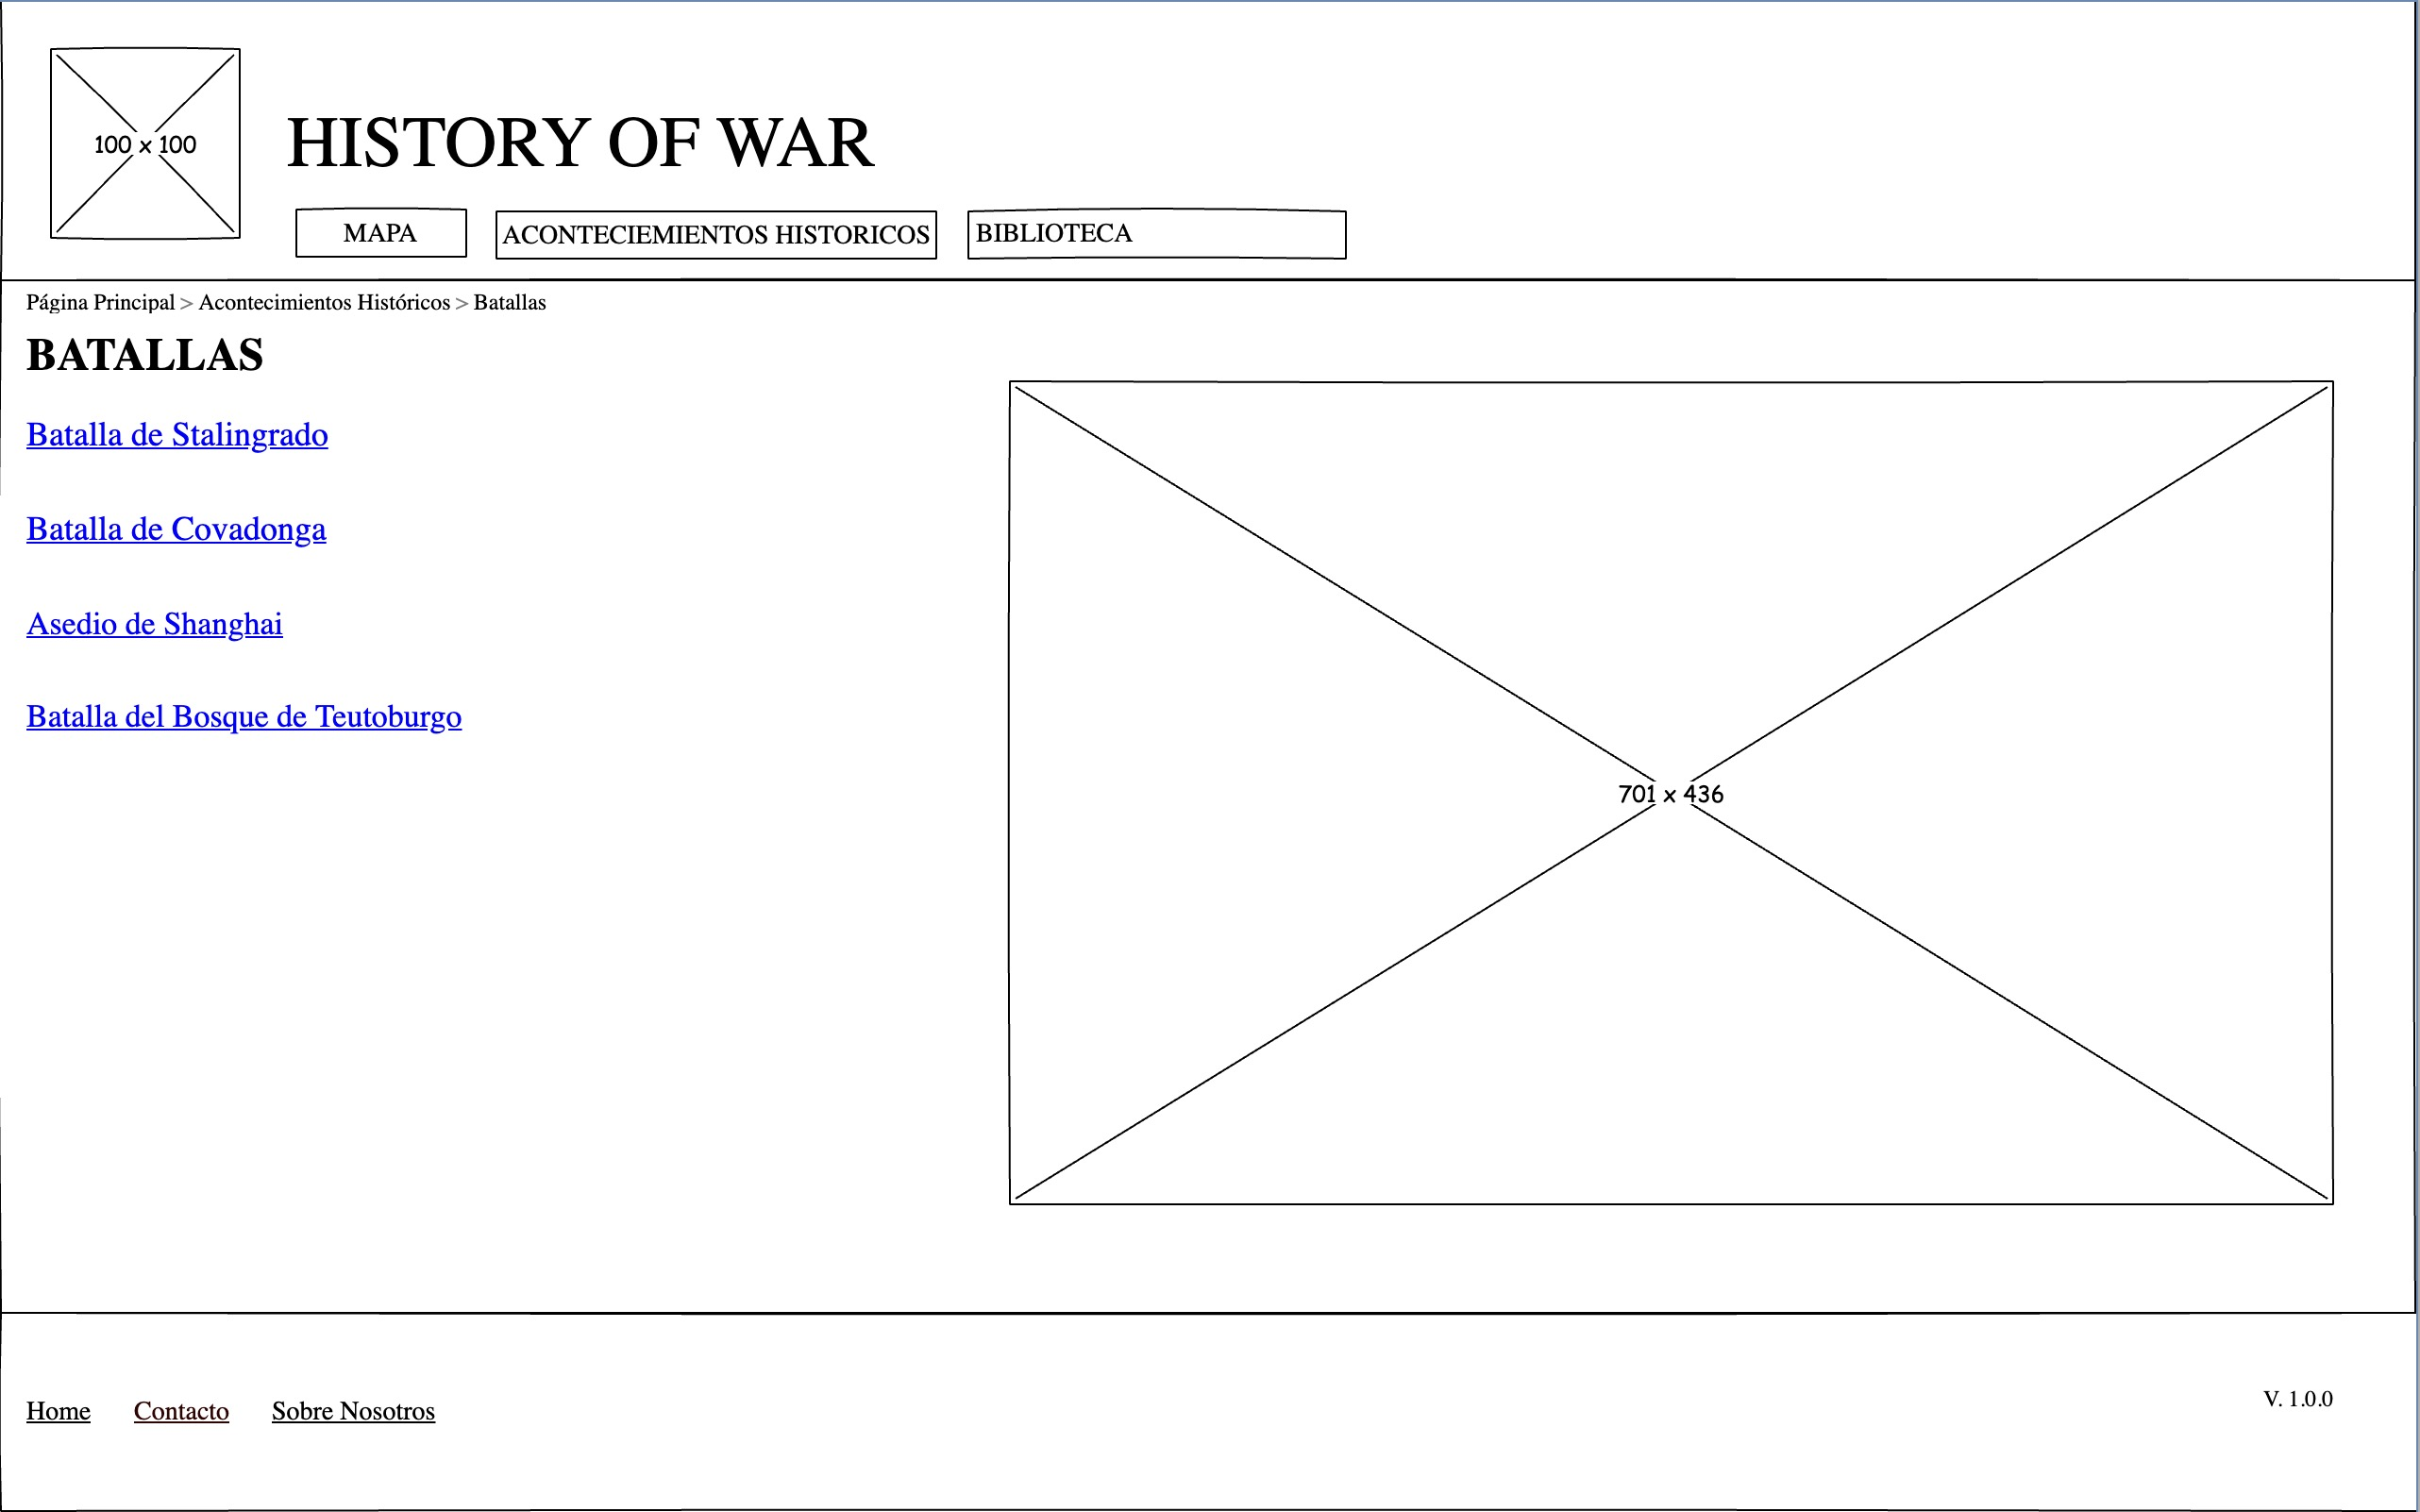
\includegraphics[width=1\textwidth]{Wireframes/Batallas.jpg}
    \caption{Batallas}
    \label{fig:mi_imagen}
\end{figure}

\begin{figure}[H]
    \centering
    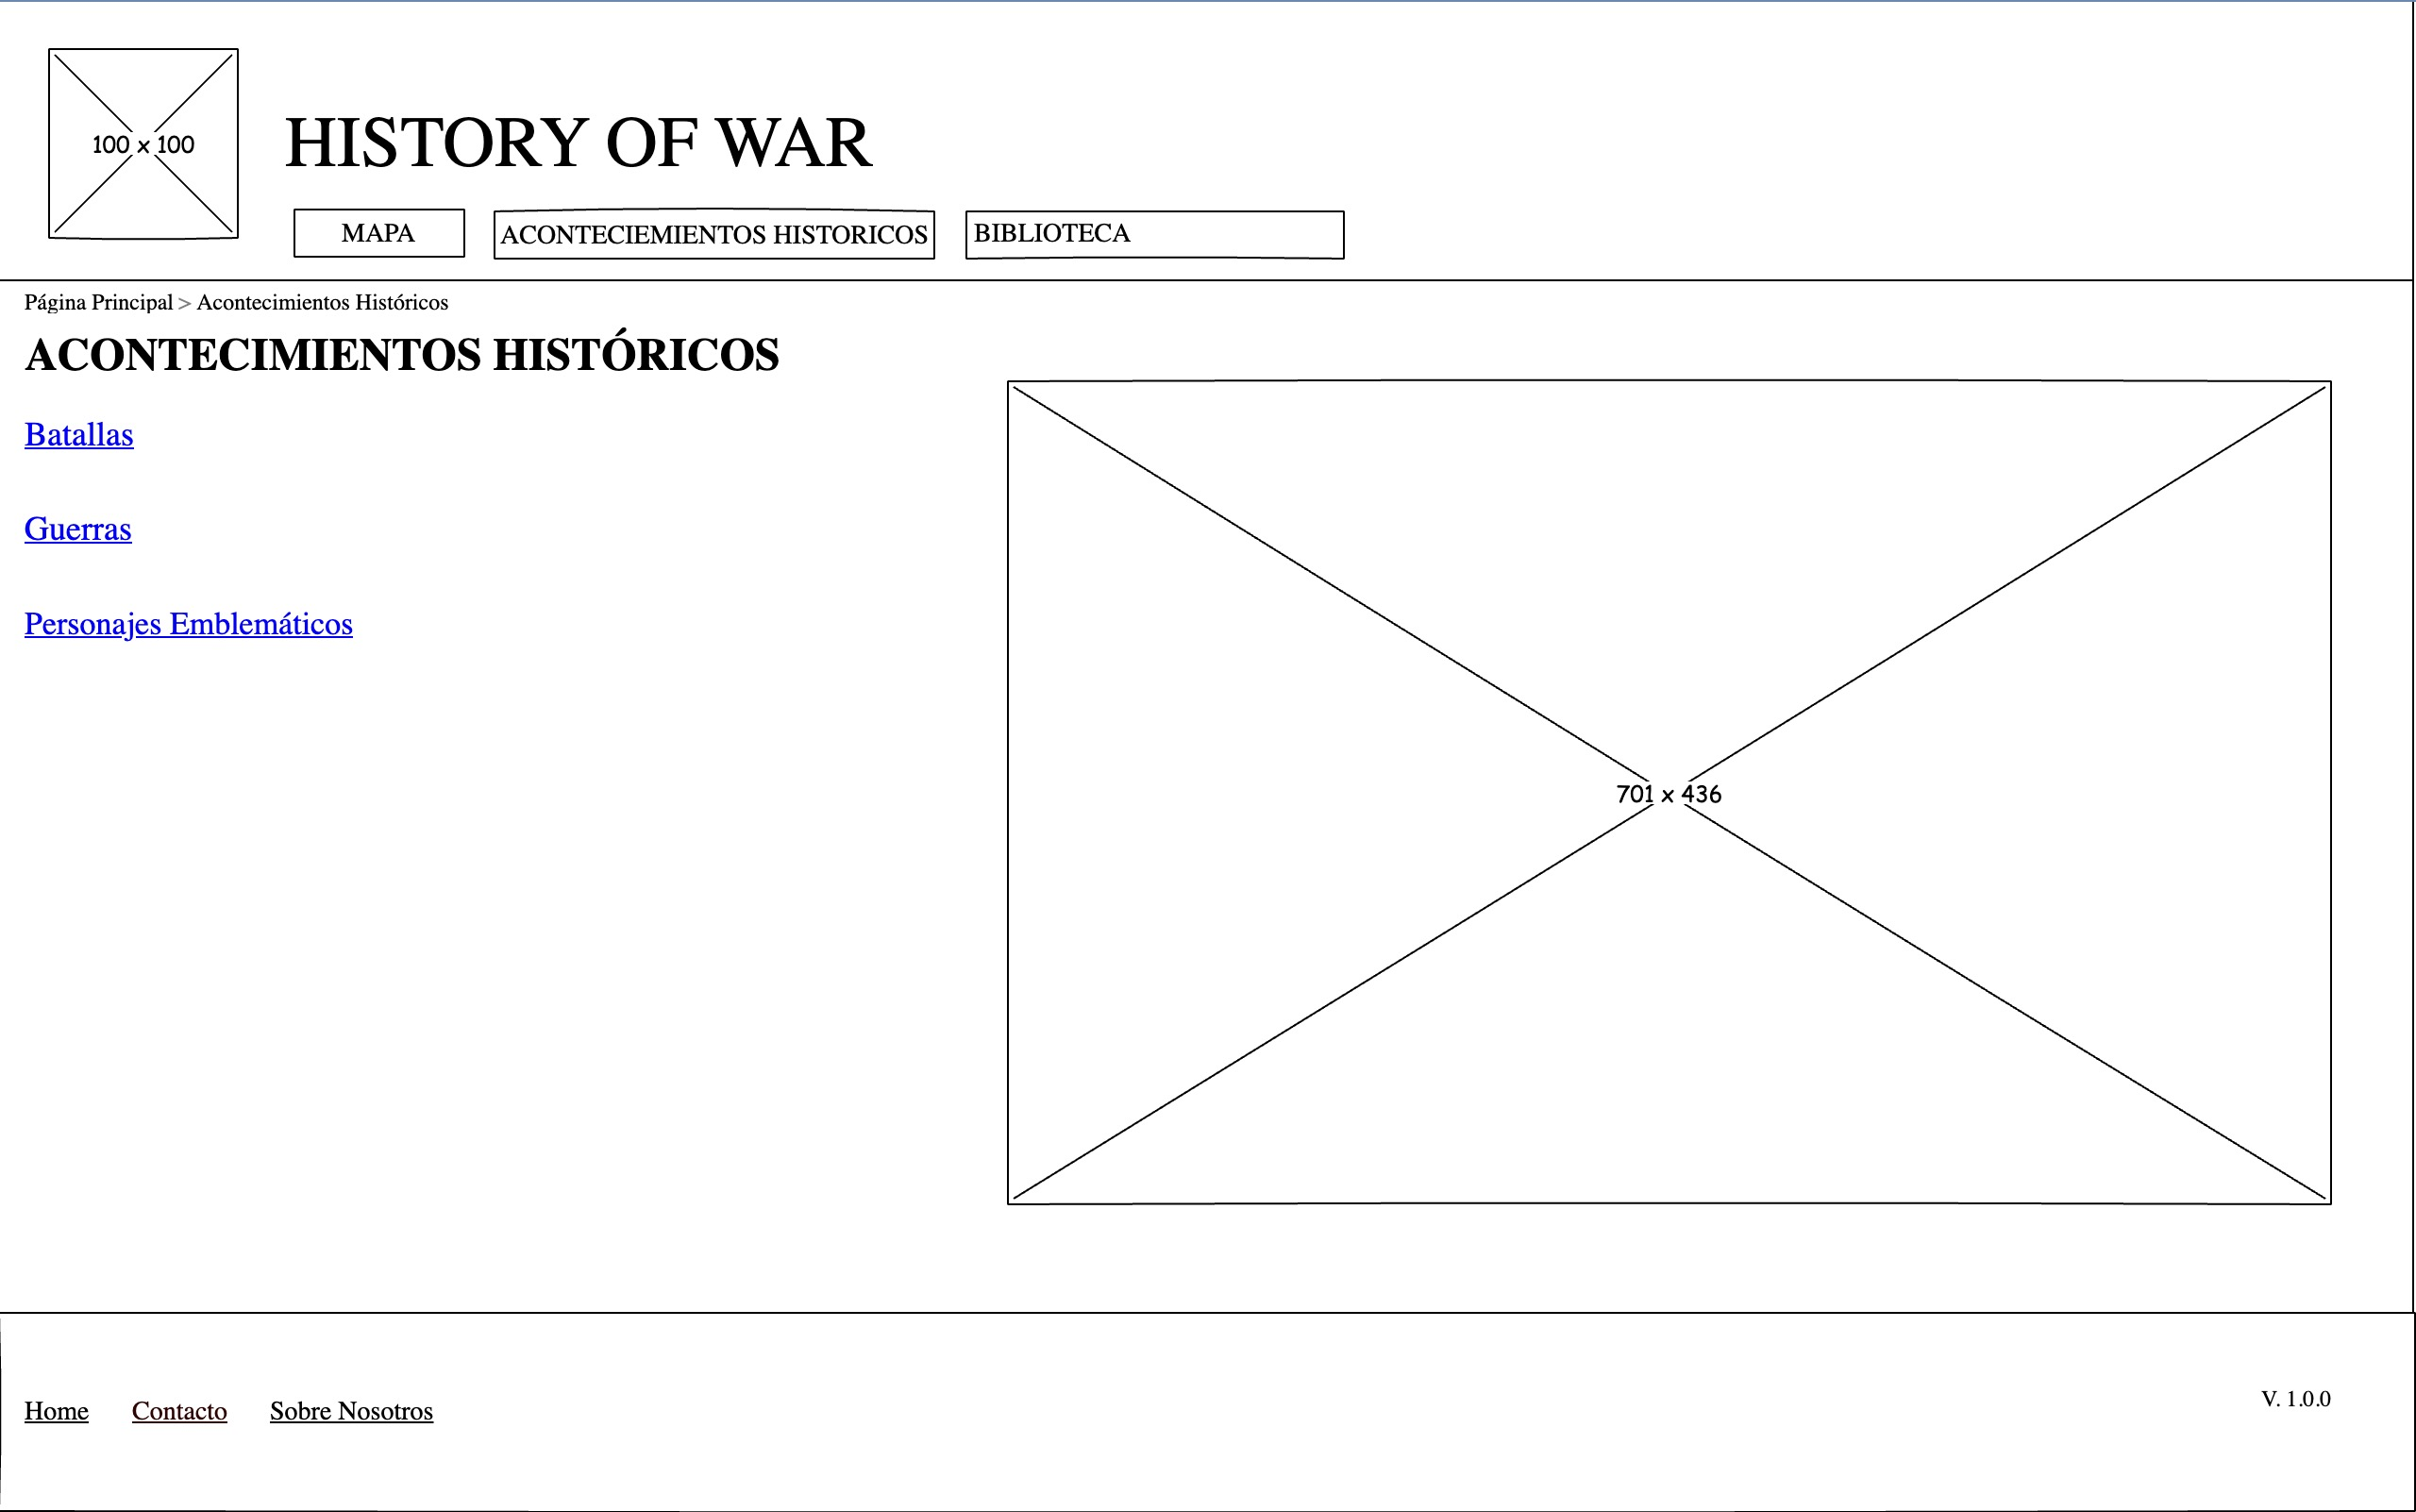
\includegraphics[width=1\textwidth]{Wireframes/AH.jpg}
    \caption{Acontecimientos Históricos}
    \label{fig:mi_imagen}
\end{figure}

\subsection{Mockups}

Los mockups son representaciones visuales de alta fidelidad que avanzan sobre la base establecida por los wireframes, ofreciendo una versión más detallada y cercana al diseño final de nuestra página web. Estas maquetas incorporan elementos de diseño gráfico, paletas de colores, tipografías y otros componentes estéticos, proporcionando una vista previa más precisa de cómo se verá y sentirá el sitio web una vez completado. Funcionan como una herramienta esencial en el proceso de diseño, facilitando la evaluación y ajuste del aspecto visual y la experiencia de usuario antes de entrar en las etapas de desarrollo técnico.

\begin{figure}[H]
    \centering
    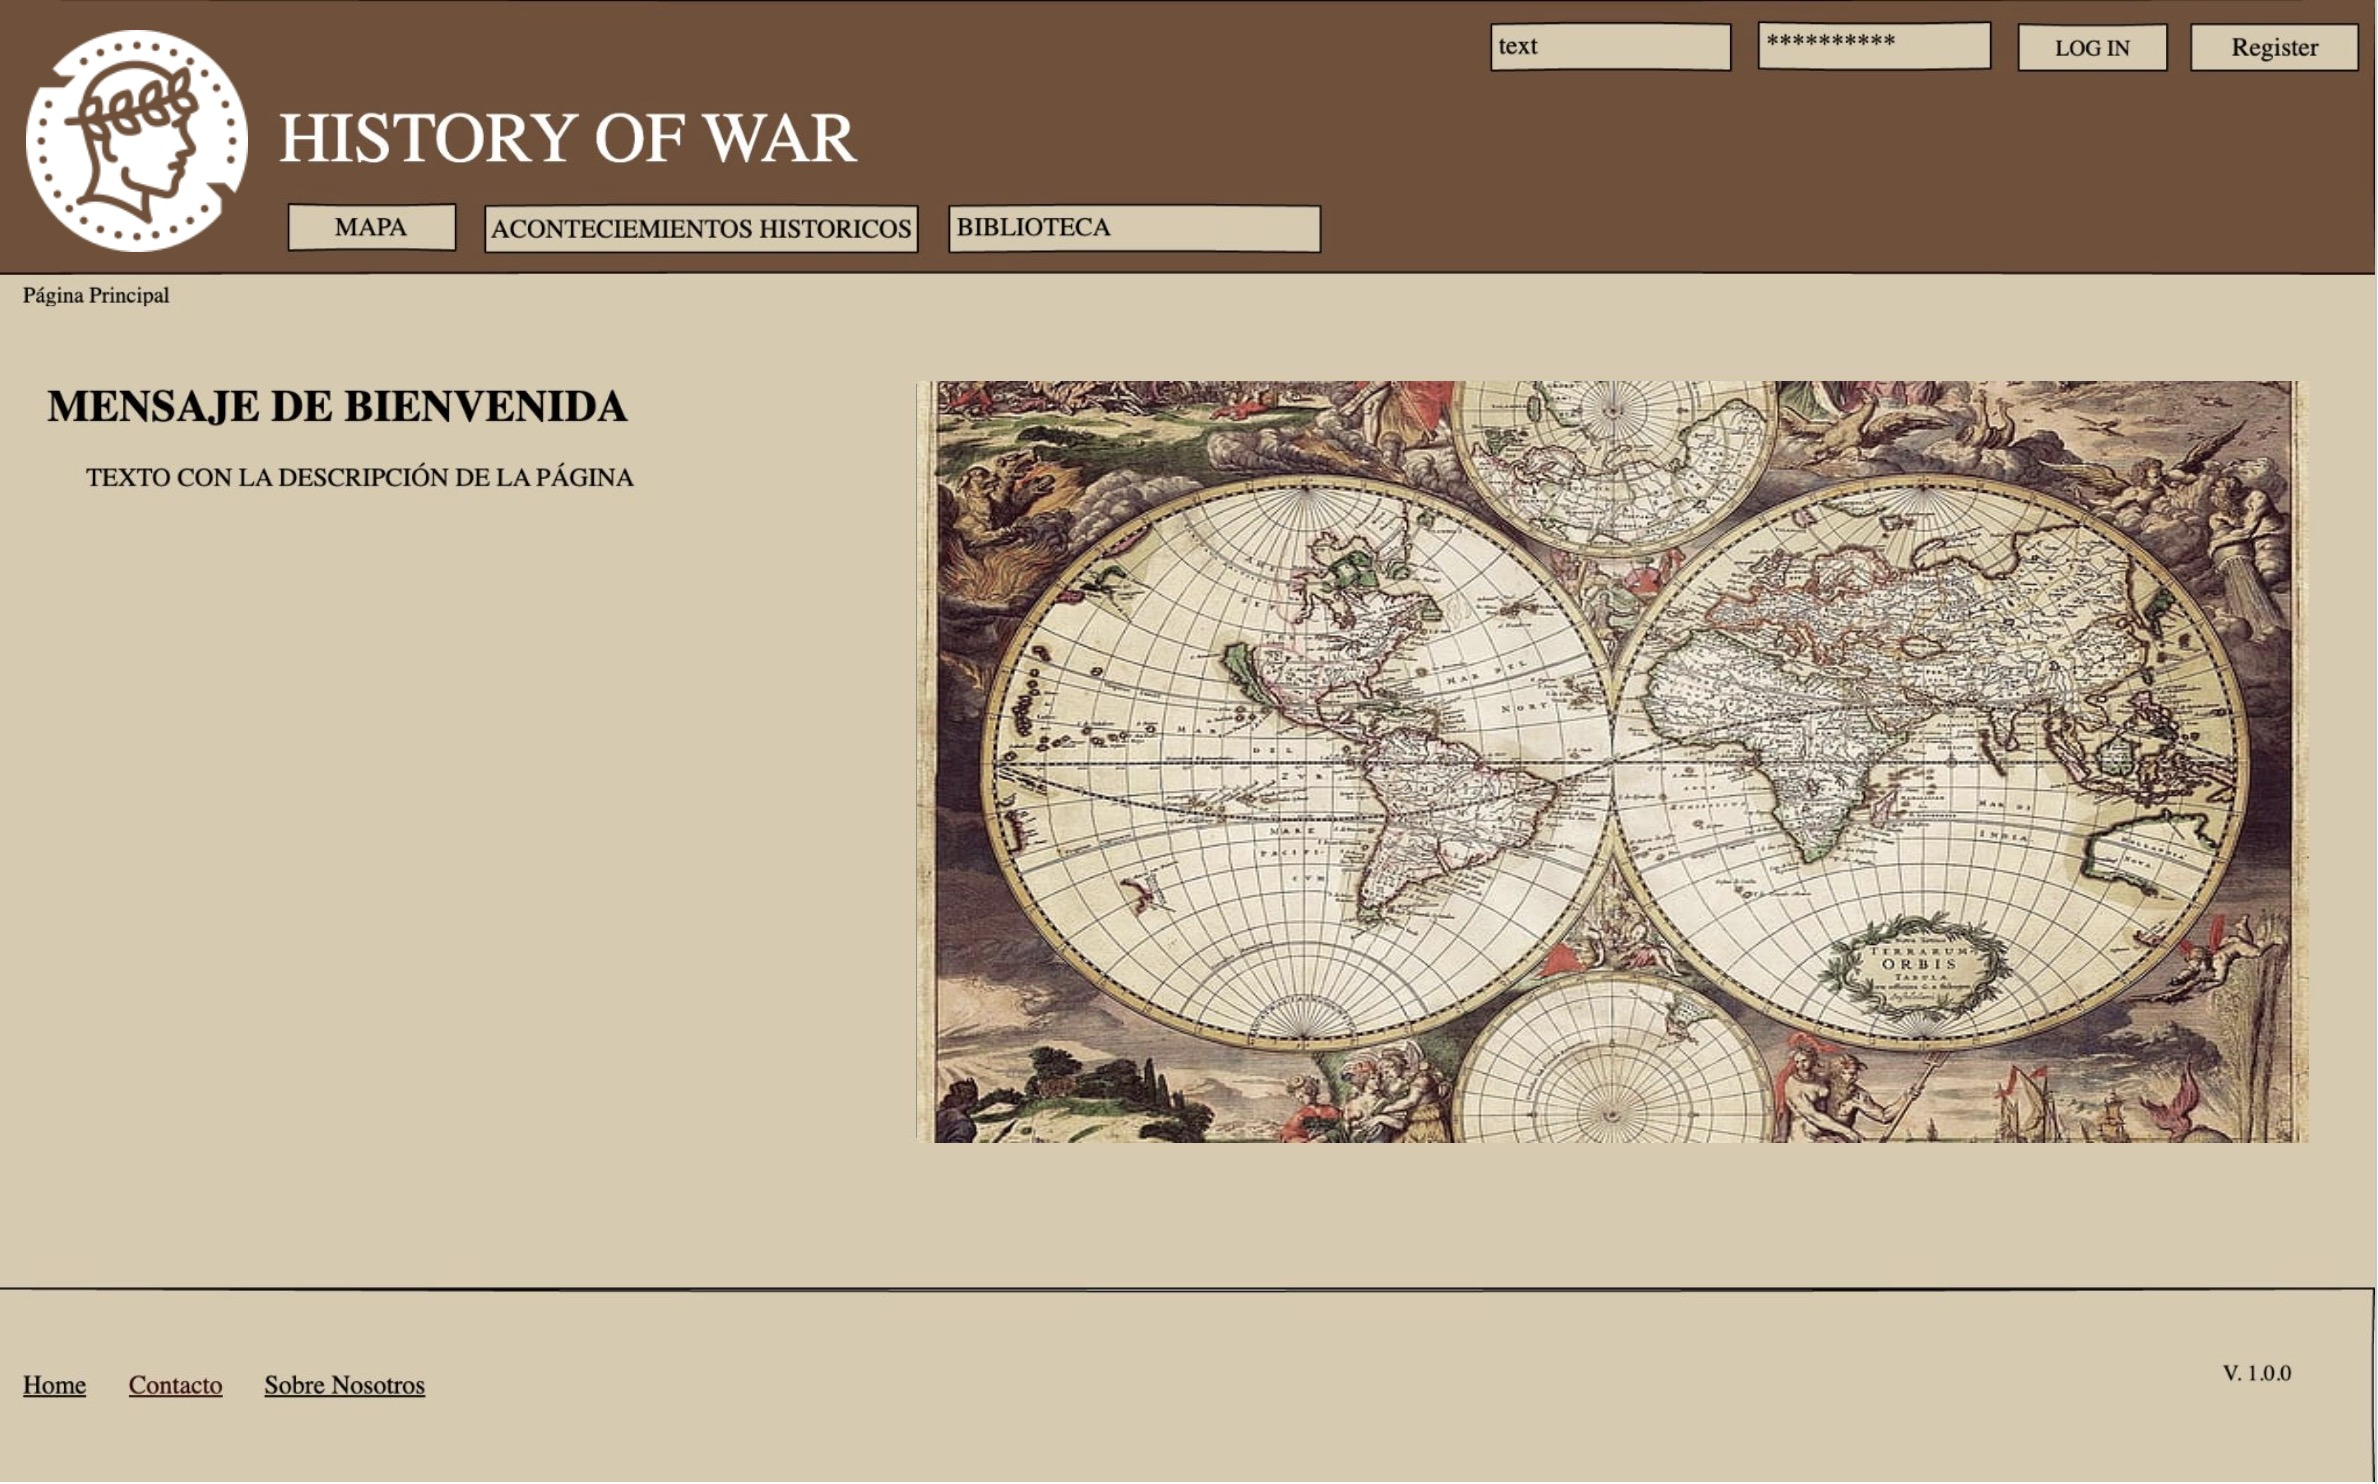
\includegraphics[width=1\textwidth]{Mockup/PaginaPrincipal (1).jpg}
    \caption{Página Principal}
    \label{fig:mi_imagen}
\end{figure}

\begin{figure}[H]
    \centering
    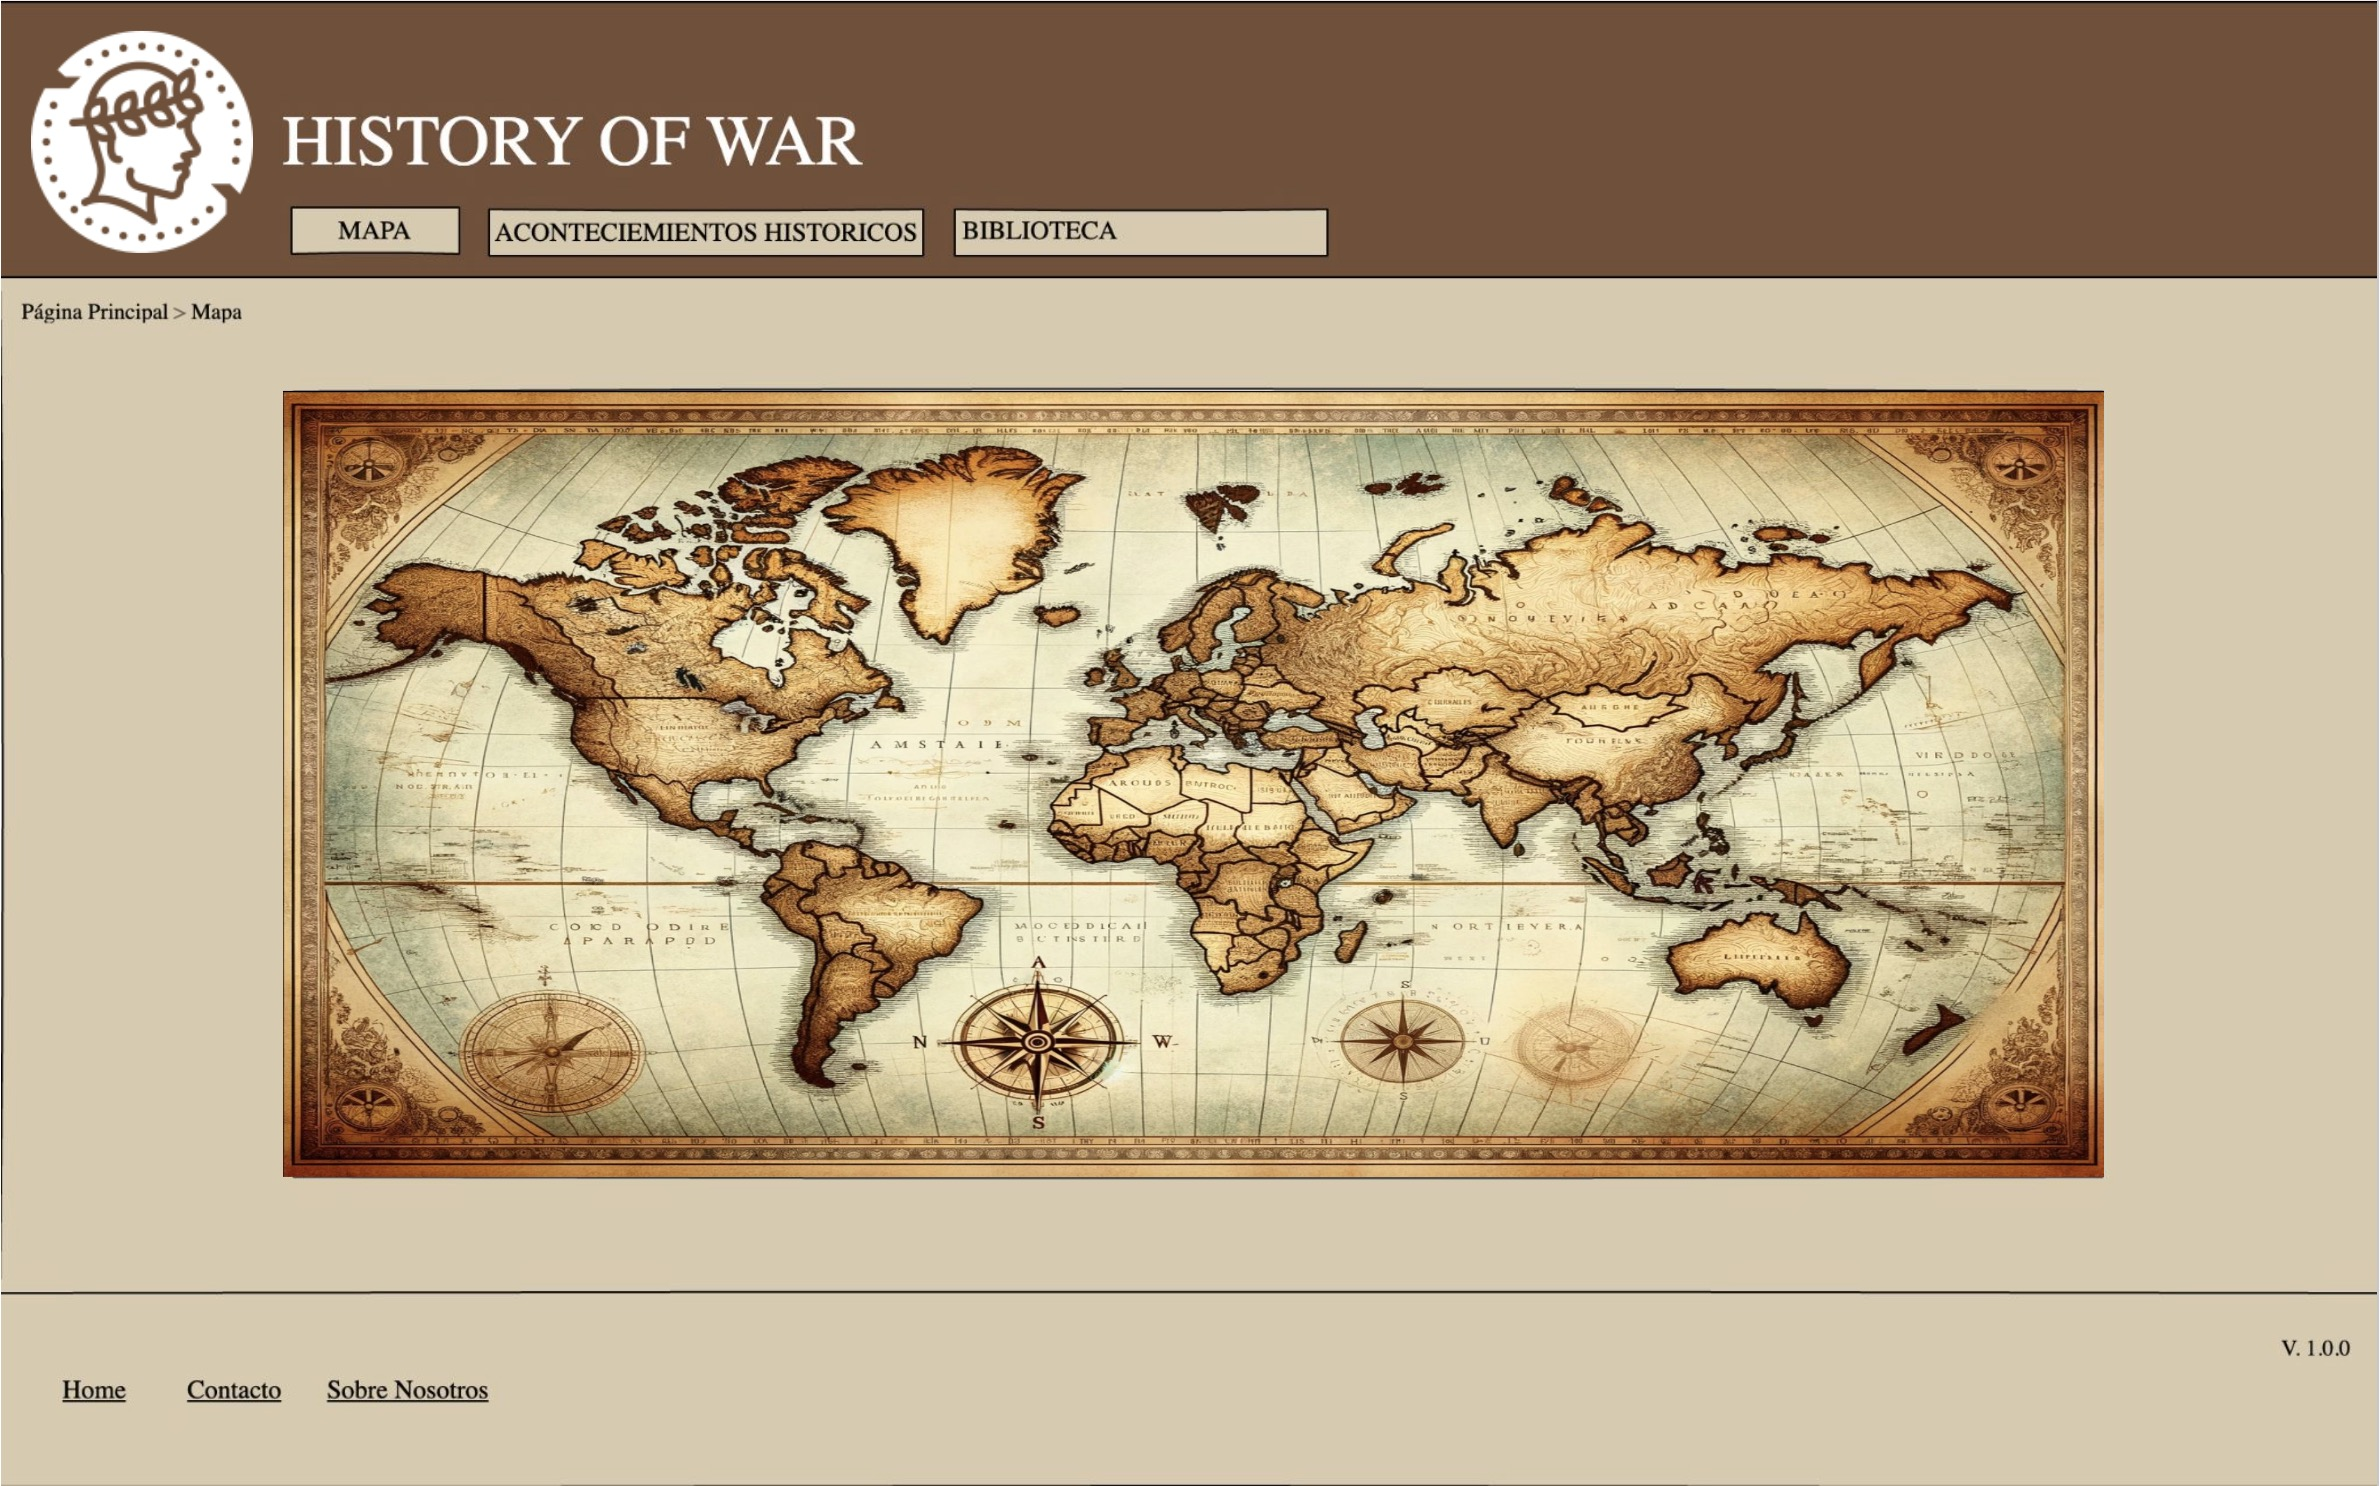
\includegraphics[width=1\textwidth]{Mockup/MapaMockup.jpg}
    \caption{Mapa}
    \label{fig:mi_imagen}
\end{figure}

\begin{figure}[H]
    \centering
    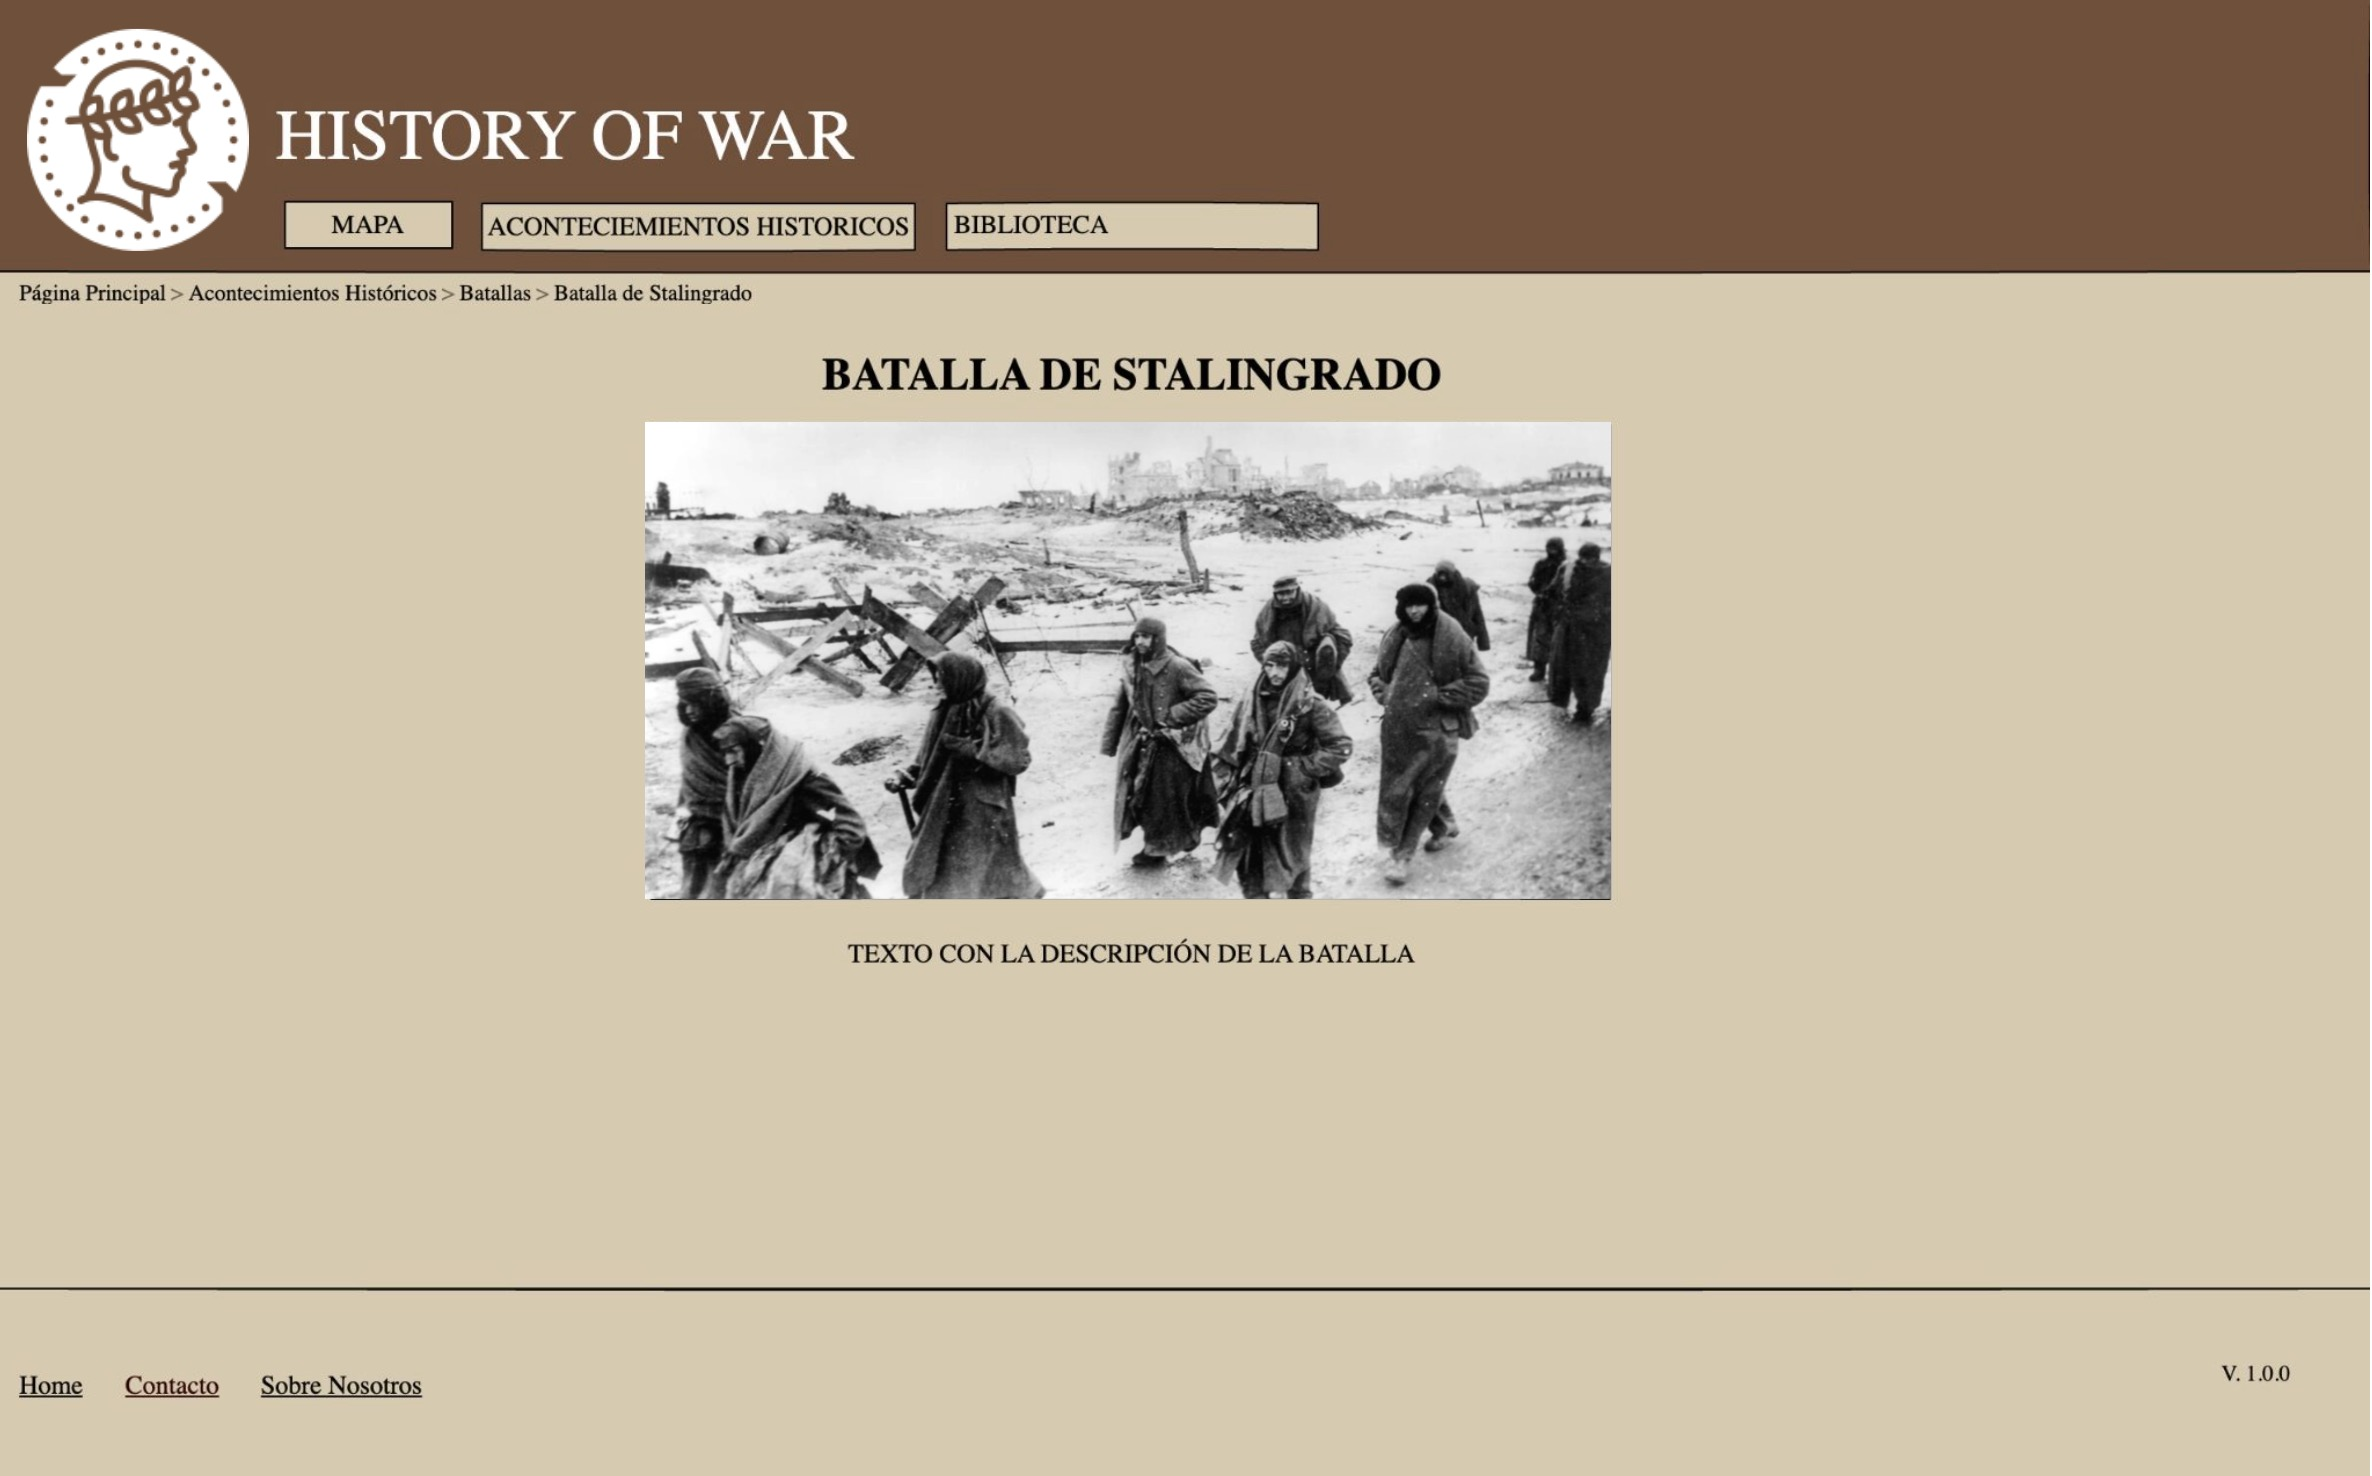
\includegraphics[width=1\textwidth]{Mockup/EjemploBatallaMockup.jpg}
    \caption{Ejemplo Batalla}
    \label{fig:mi_imagen}
\end{figure}

\begin{figure}[H]
    \centering
    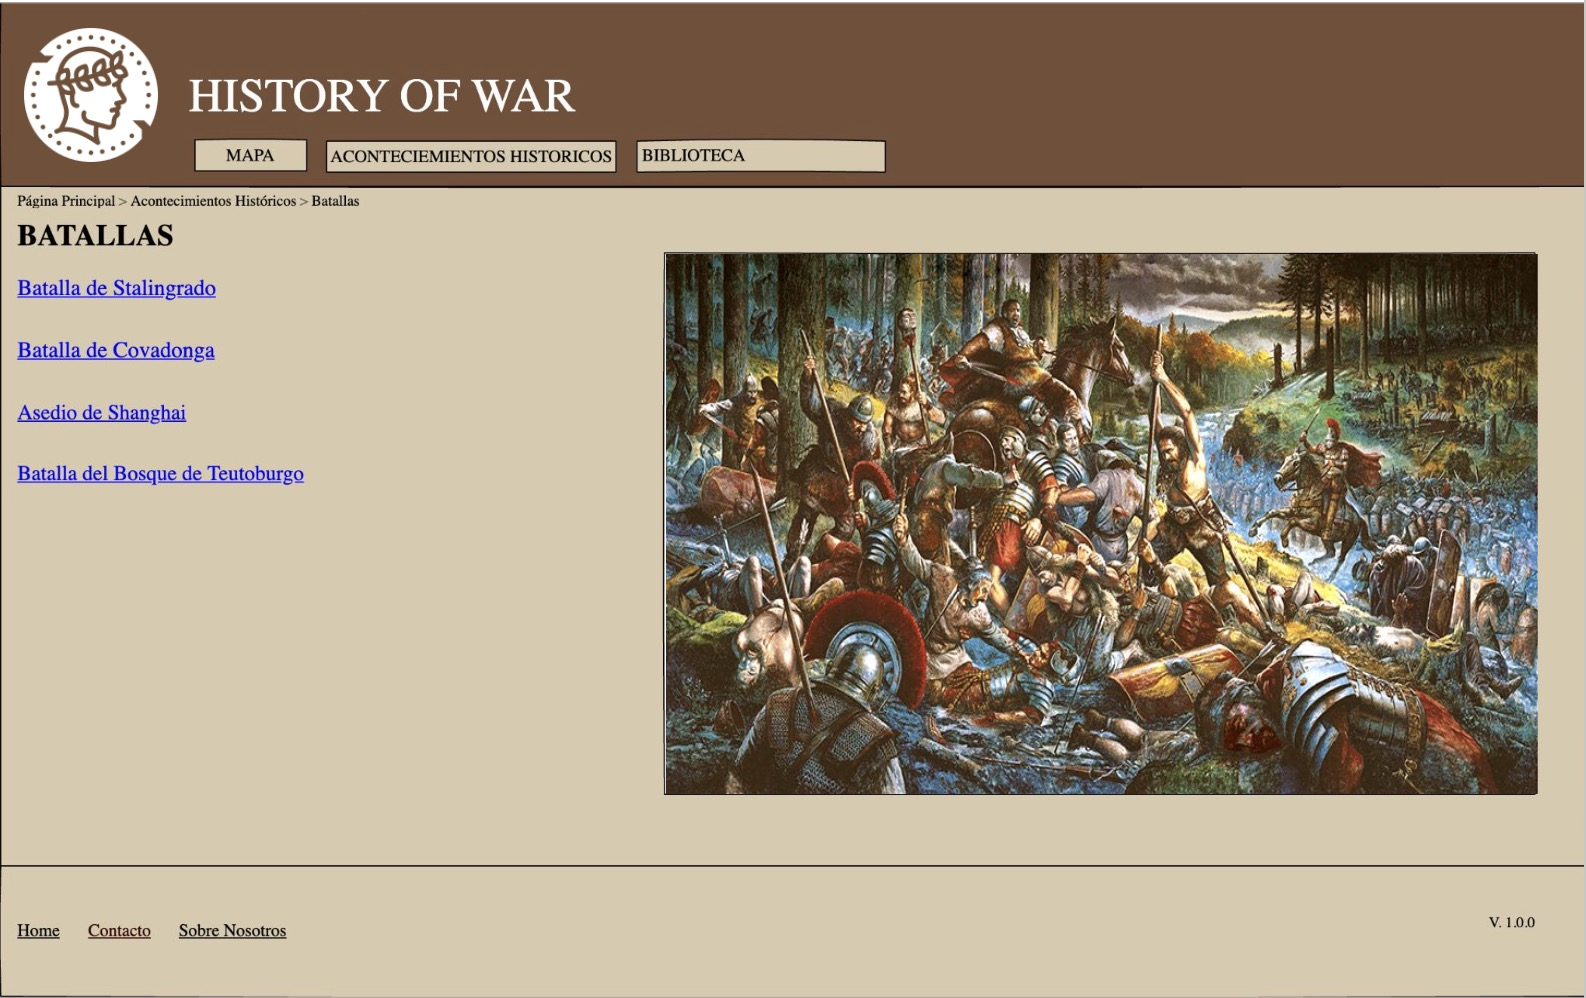
\includegraphics[width=1\textwidth]{Mockup/BatallasMockup.jpg}
    \caption{Batallas}
    \label{fig:mi_imagen}
\end{figure}

\begin{figure}[H]
    \centering
    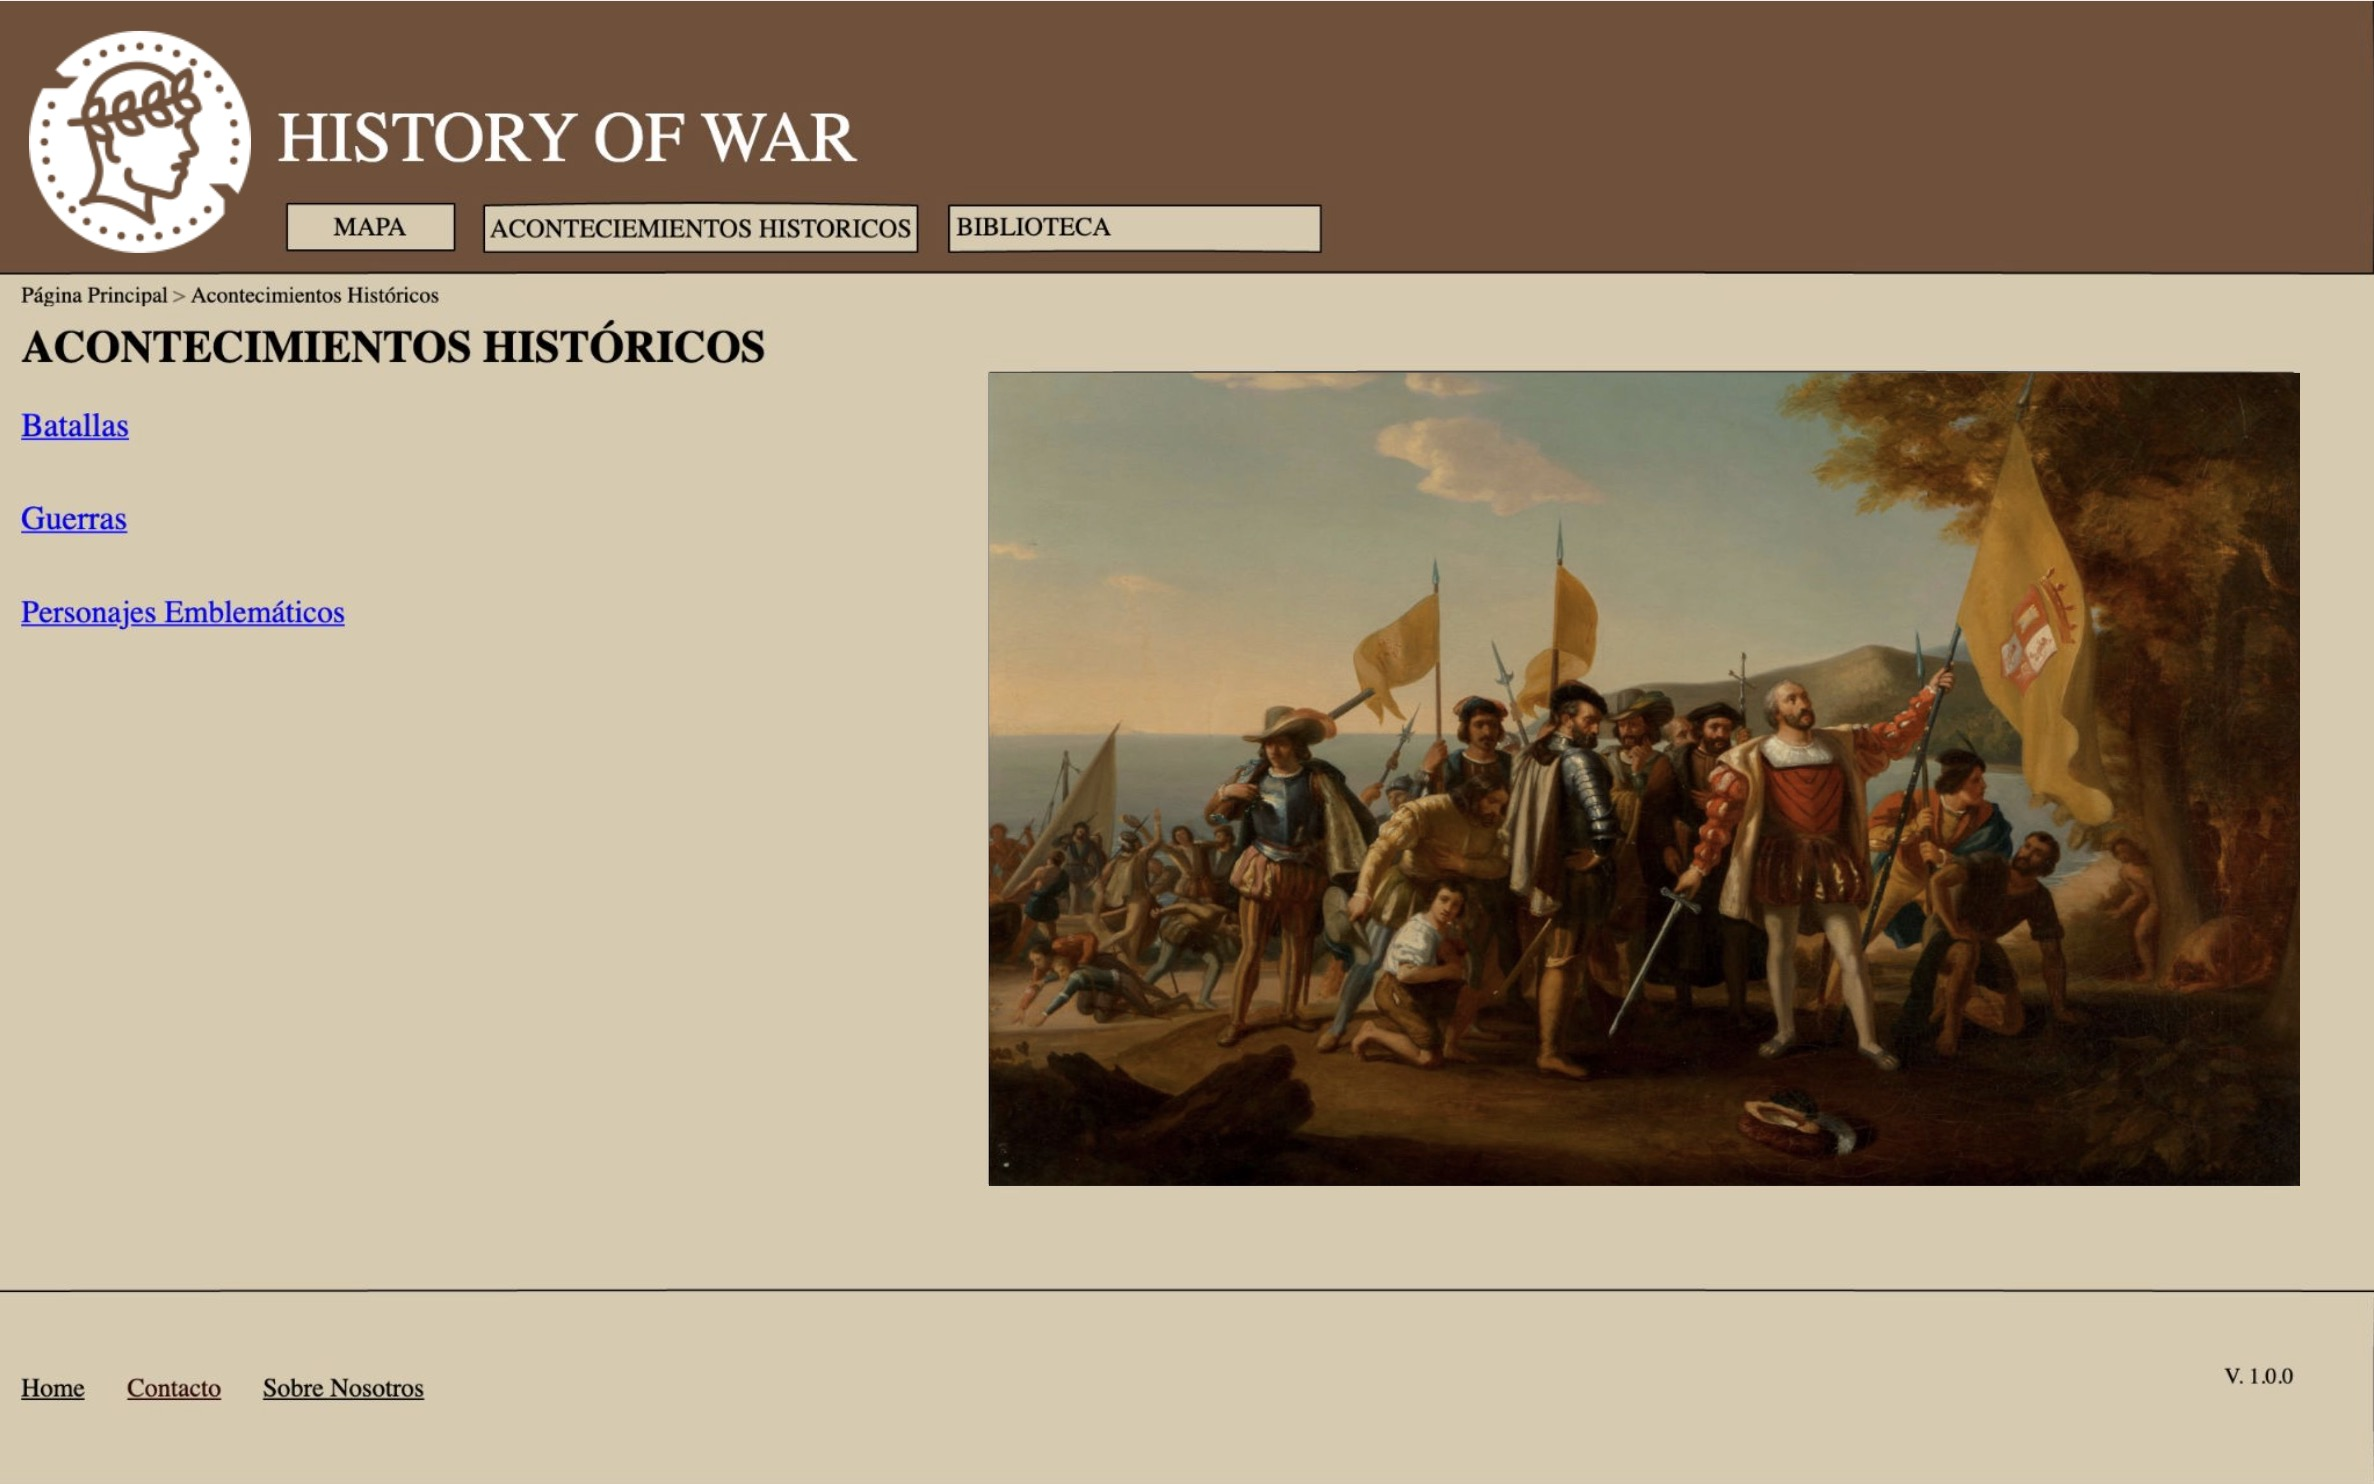
\includegraphics[width=1\textwidth]{Mockup/AHMockup.jpg}
    \caption{Acontecimientos Históricos}
    \label{fig:mi_imagen}
\end{figure}

\newpage

\section{Storyboards}

Son secuencias narrativas visuales que ilustran el flujo y la experiencia del usuario al interactuar con la página web. Estos diagramas cuentan la "historia" de cómo un usuario típico podría navegar a través del sitio, desde la página de inicio hasta la realización de acciones específicas, como realizar una compra, inscribirse en un servicio o encontrar información relevante.

\begin{figure}[H]
    \centering
    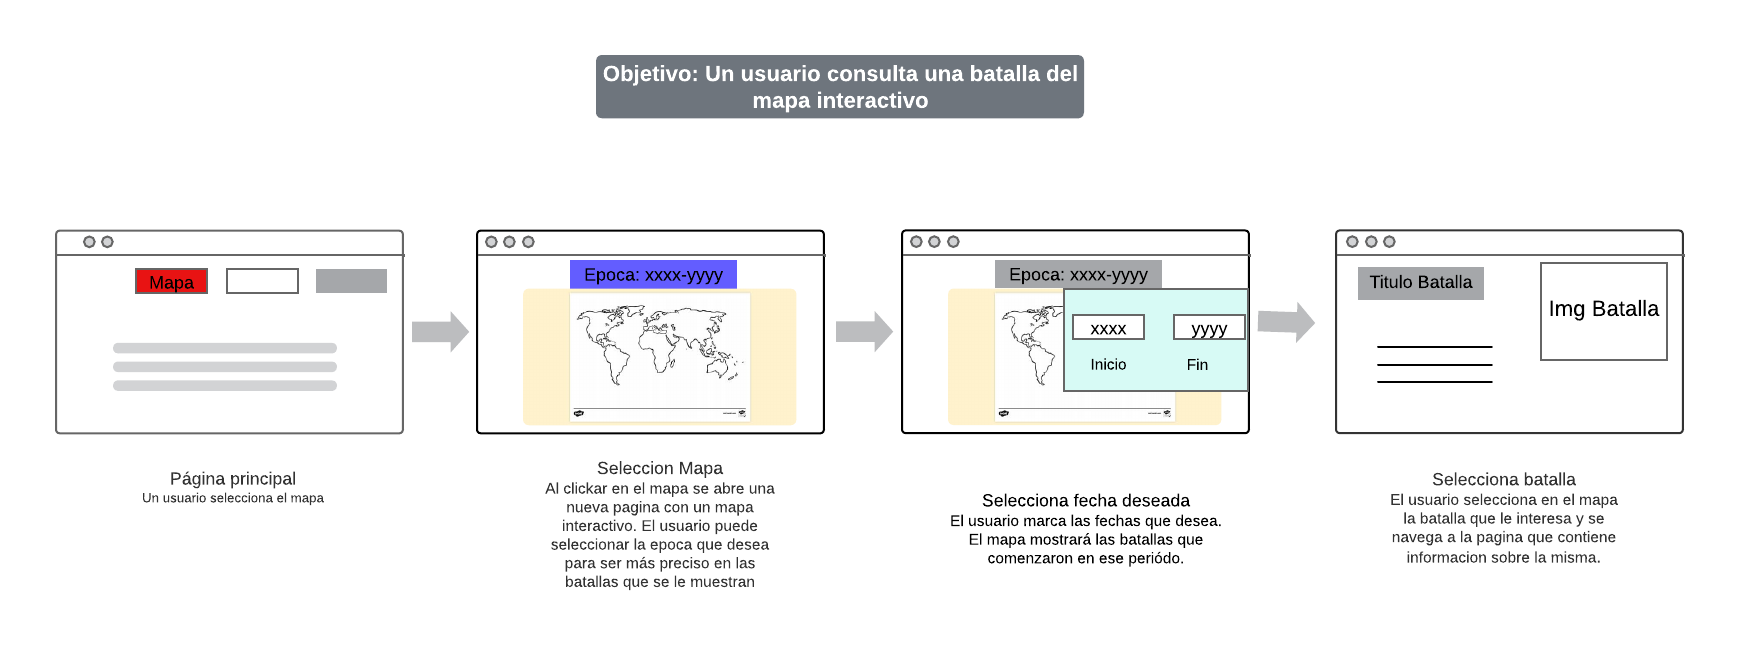
\includegraphics[width=1\textwidth]{Storyboards/StoryBoard_seleccion_batalla.png}
    \caption{Selección de Batalla}
    \label{fig:mi_imagen}
\end{figure}

\begin{figure}[H]
    \centering
    \includegraphics[width=1\textwidth]{Storyboards/StoryBoard_seleccion_libro.png}
    \caption{Selección de Libro}
    \label{fig:mi_imagen}
\end{figure}

\begin{figure}[H]
    \centering
    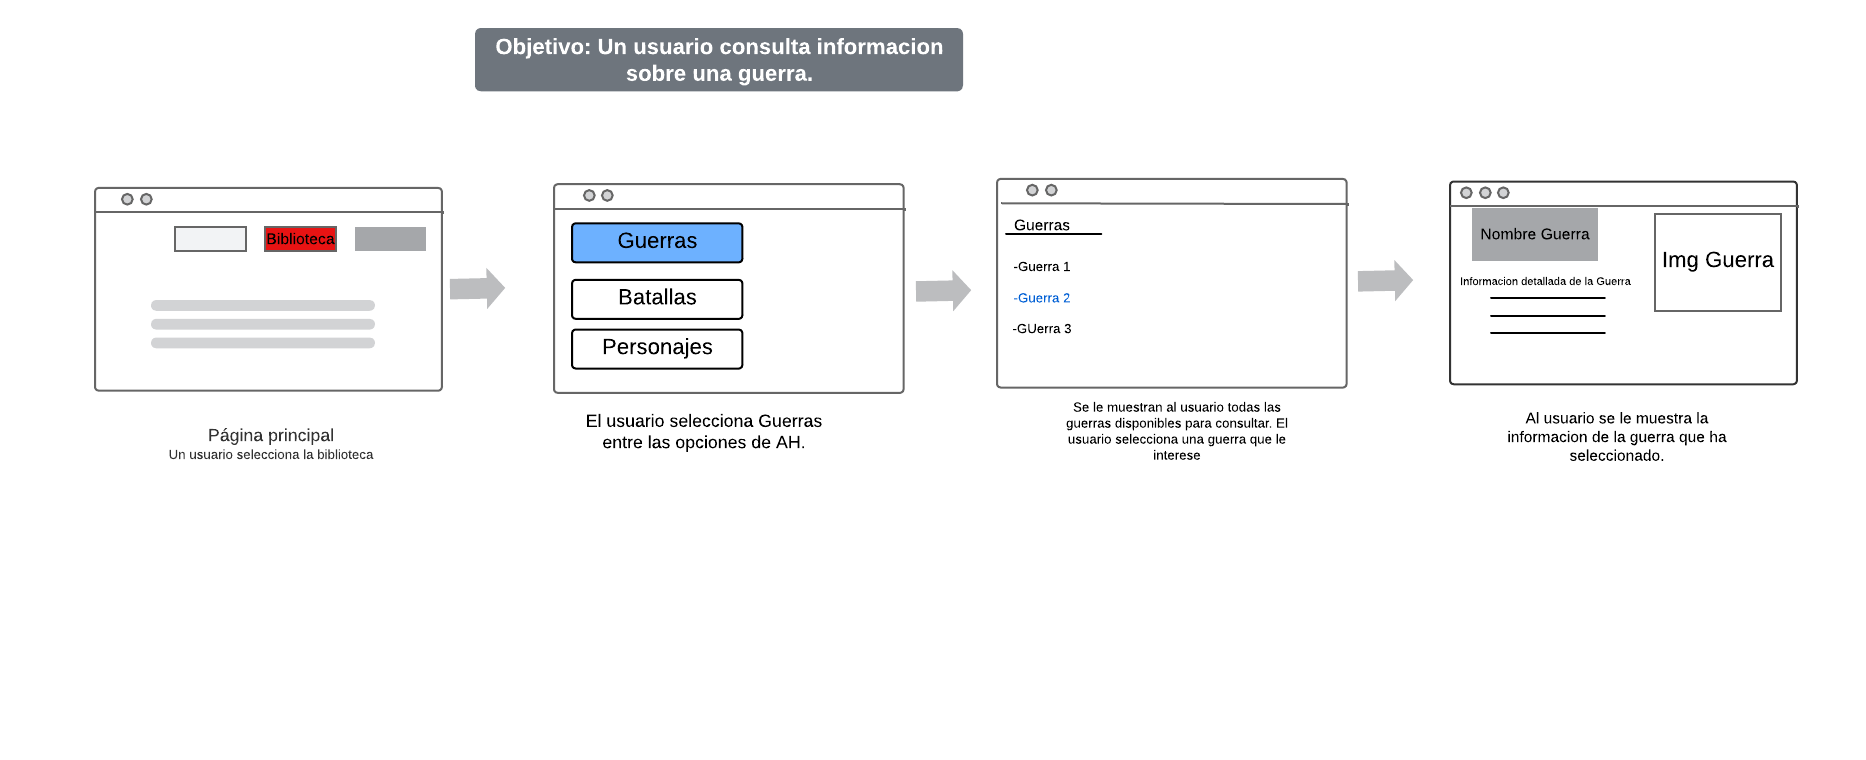
\includegraphics[width=1\textwidth]{Storyboards/StoryBoard_seleccion_guerra.png}
    \caption{Selección de Guerra}
    \label{fig:mi_imagen}
\end{figure}

\begin{figure}[H]
    \centering
    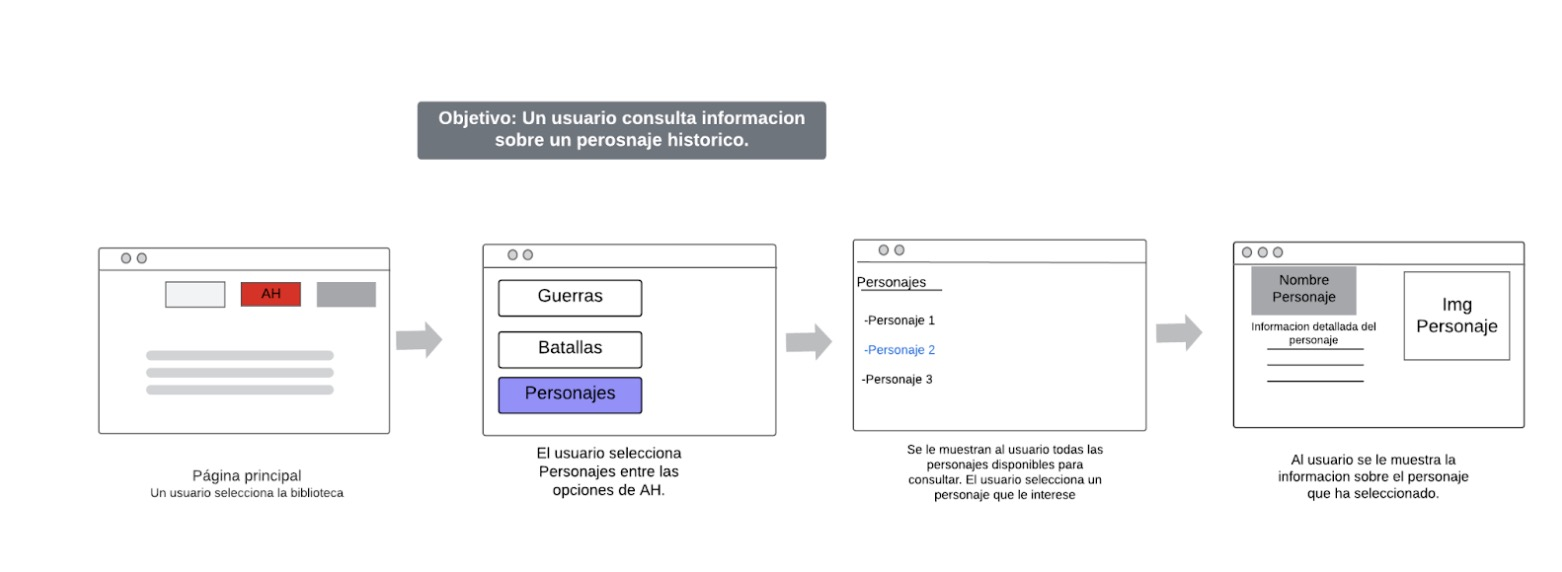
\includegraphics[width=1\textwidth]{Storyboards/StoryboardPersonaje.jpg}
    \caption{Selección de Personaje}
    \label{fig:mi_imagen}
\end{figure}

\begin{figure}[H]
    \centering
    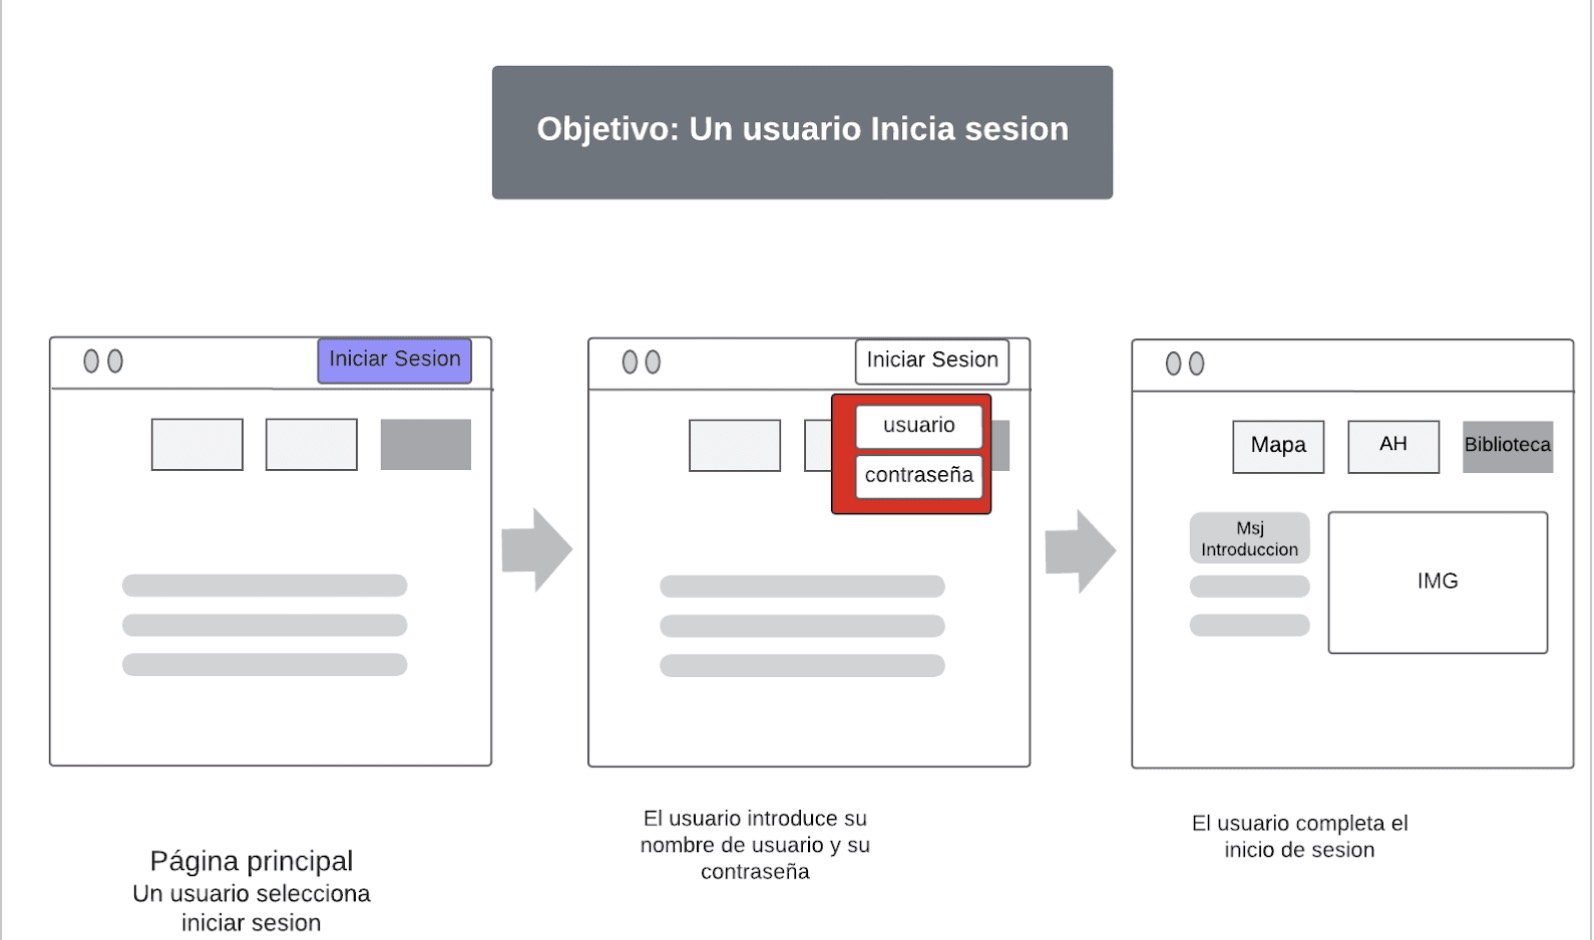
\includegraphics[width=1\textwidth]{Storyboards/StroryBoardInicioSesion.jpg}
    \caption{Inicio de Sesión}
    \label{fig:mi_imagen}
\end{figure}

\newpage

\section{Estructura de Ficheros y Carpetas}

La estructura de ficheros y carpetas en un proyecto web es esencial para mantener el orden y facilitar el desarrollo y mantenimiento del sitio. Esta organización comprende la disposición sistemática de archivos HTML, hojas de estilo CSS, scripts de JavaScript, imágenes, fuentes y otros recursos digitales.

\begin{figure}[H]
    \centering
    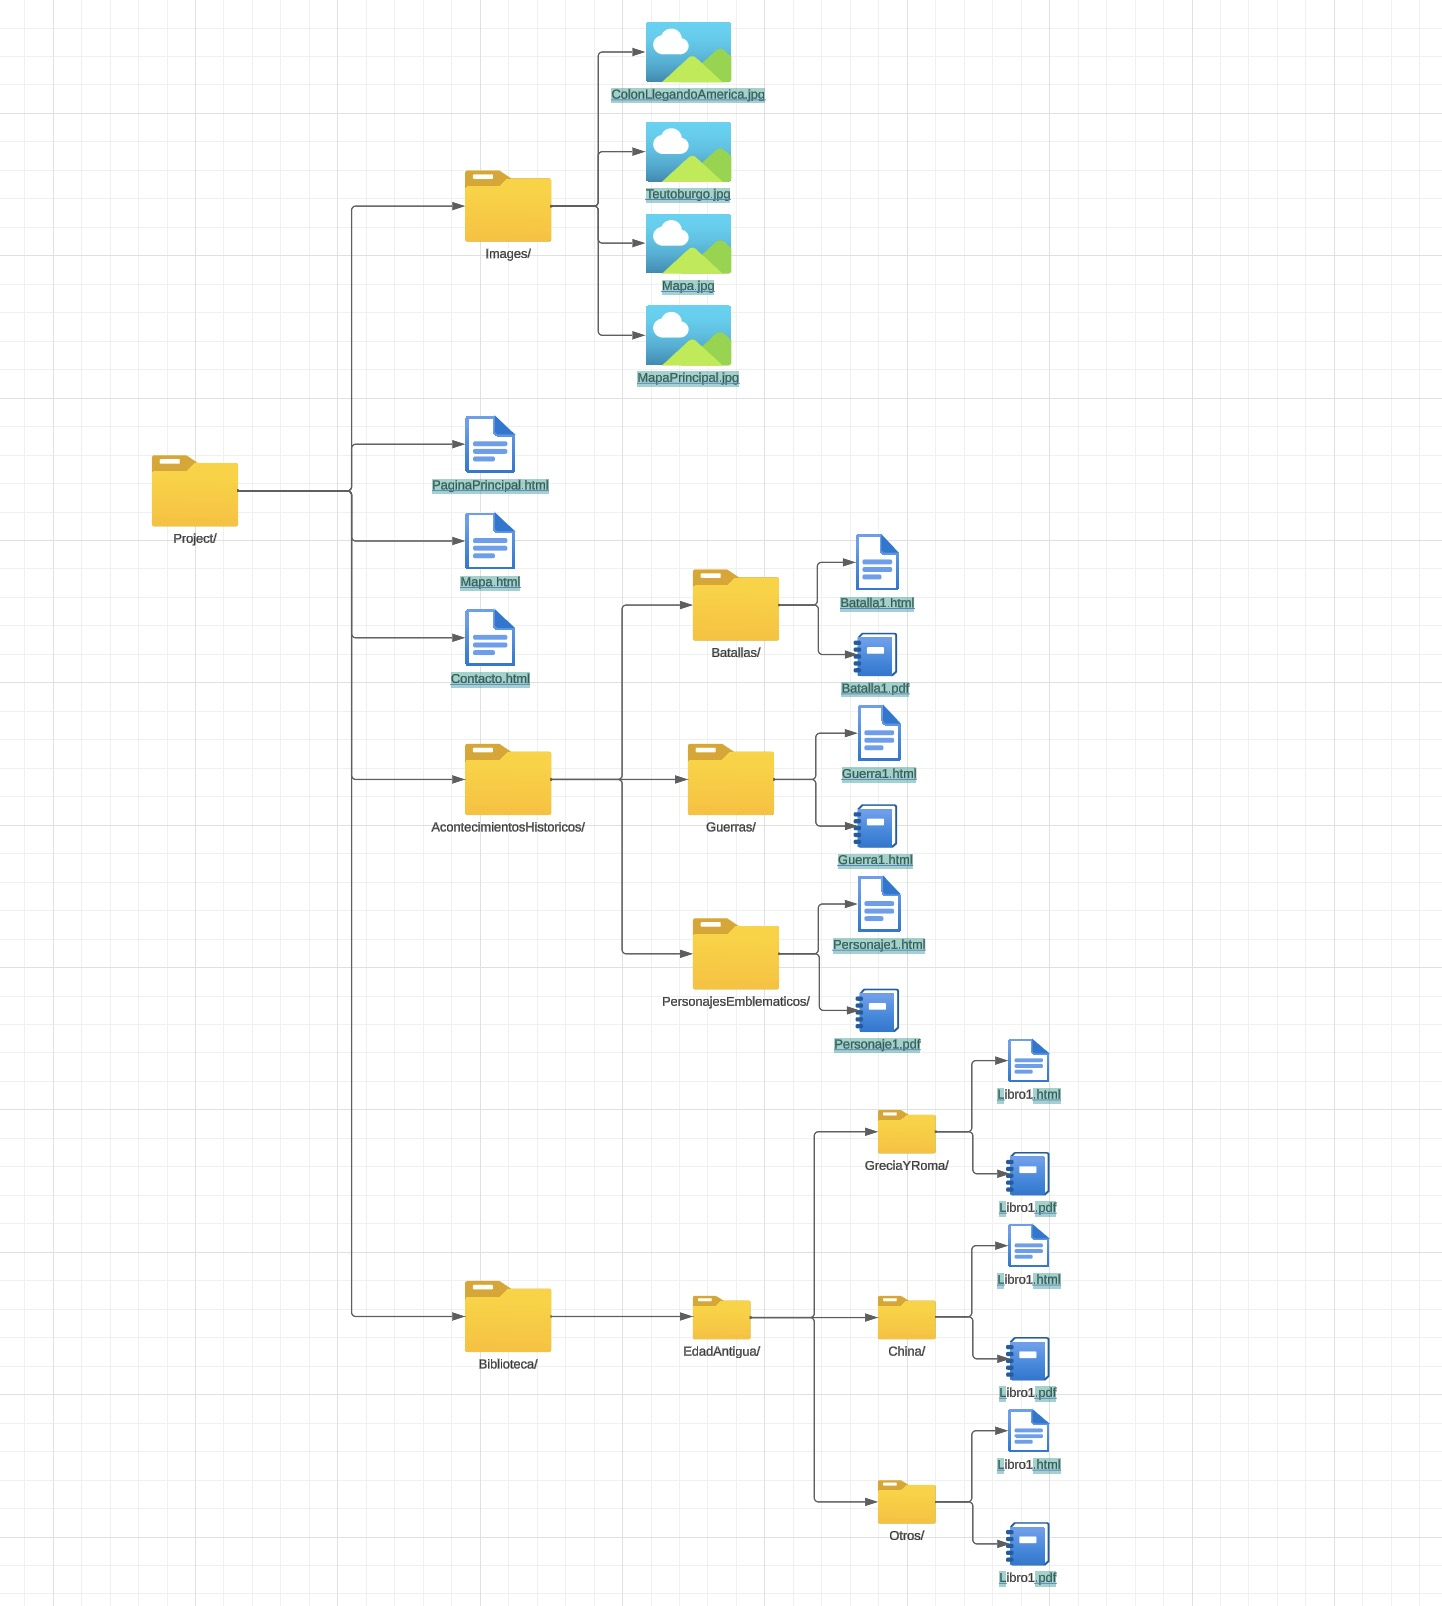
\includegraphics[width=1\textwidth]{Esquemas/EstructuraDeFicheros.jpg}
    \caption{Estructura de Ficheros y Carpetas}
    \label{fig:mi_imagen}
\end{figure}

Este esquema nos proporciona una vista general de como será la estructura que compondrá la página web, siendo extendida en la parte de la biblioteca, donde solo hemos metido una de las carpetas para ilustrar como será para todas ellas.

\newpage

\section{HTML}

Con la evolución del proyecto, las páginas modeladas al comienzo de este también fueron sujetas a cambios, por lo que en esta sección presentamos las páginas HTML finales, de las cinco partes mas significativas de nuestra web.

\subsection{Mapa de etiquetas}

\subsubsection*{index.html}

Esta es la página principal de nuestra web, donde se muestra un mensaje de bienvenida y se da acceso a las distintas secciones de la página.

\begin{figure}[H]
    \centering
    % Primera imagen (izquierda)
    \begin{minipage}{0.49\textwidth}
        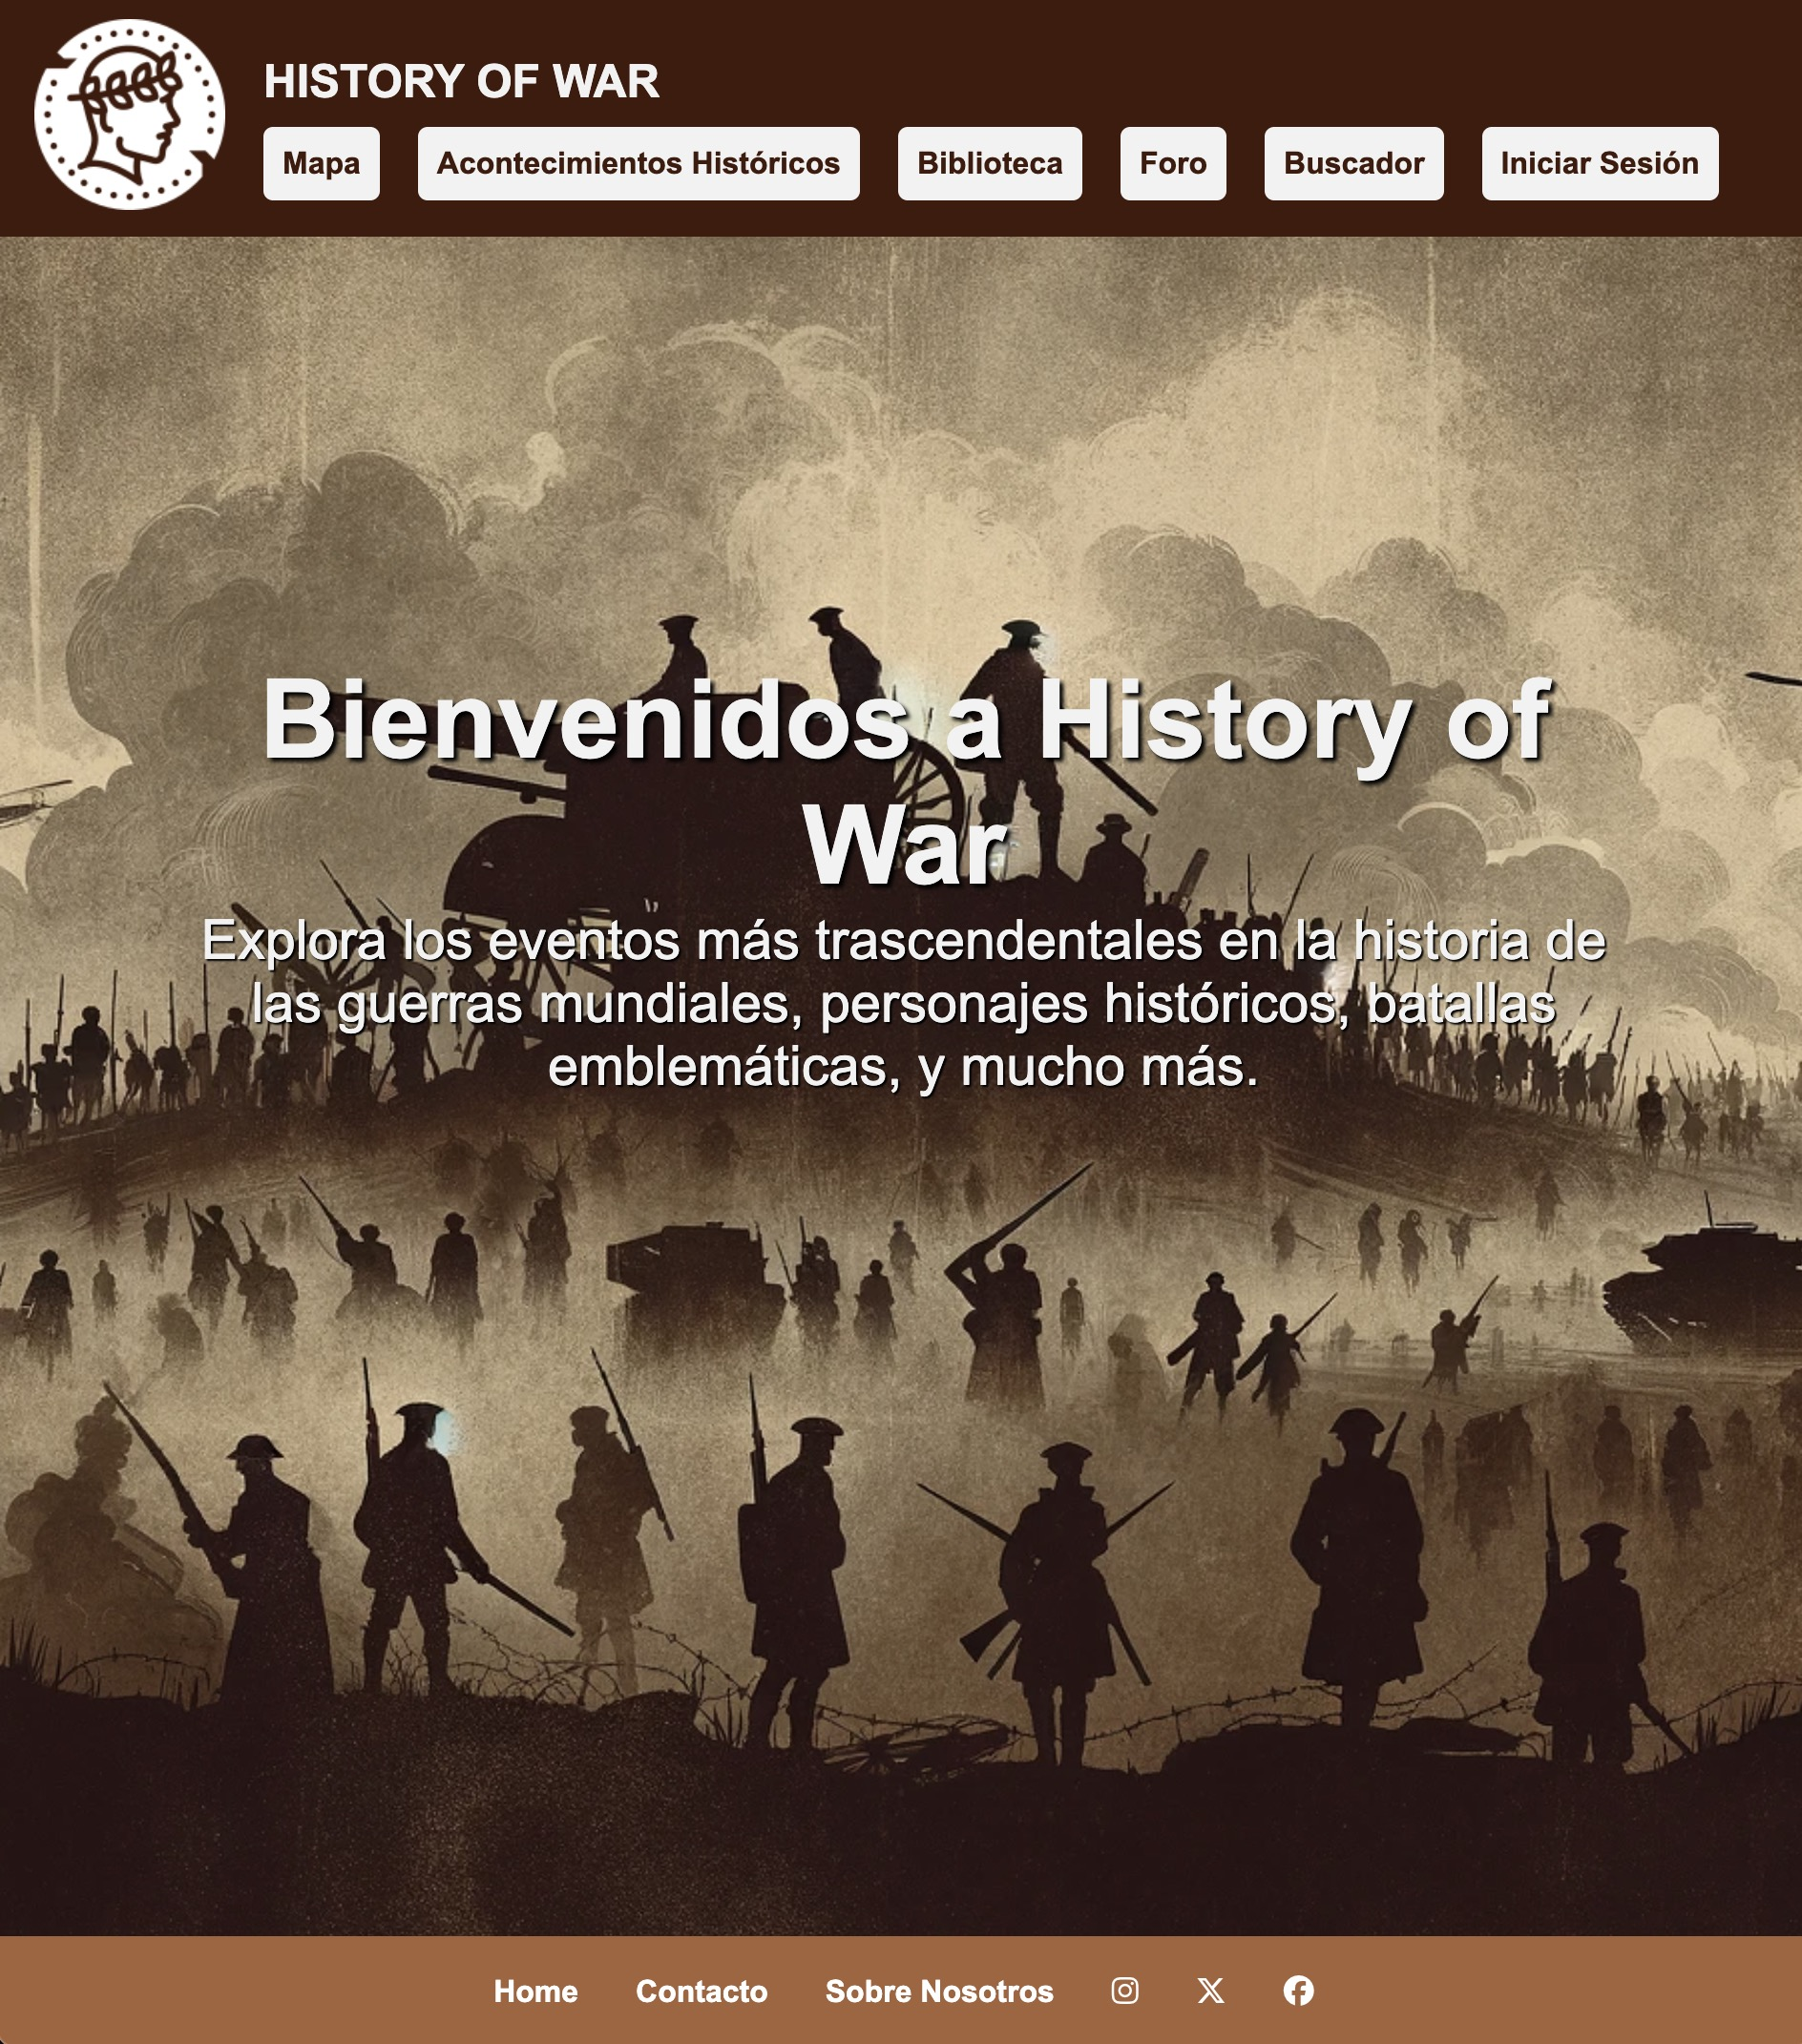
\includegraphics[width=\linewidth]{htmlFotos/pagPrincipal.png}
    \end{minipage}\hfill
    % Segunda imagen (derecha)
    \begin{minipage}{0.49\textwidth}
        \includegraphics[width=\linewidth]{htmlFotos/prototipoPagPrincipal.png}
    \end{minipage}
    
    % Ajuste de espacio vertical si es necesario
    \vspace{5mm}
    
    % Tercera imagen (debajo)
    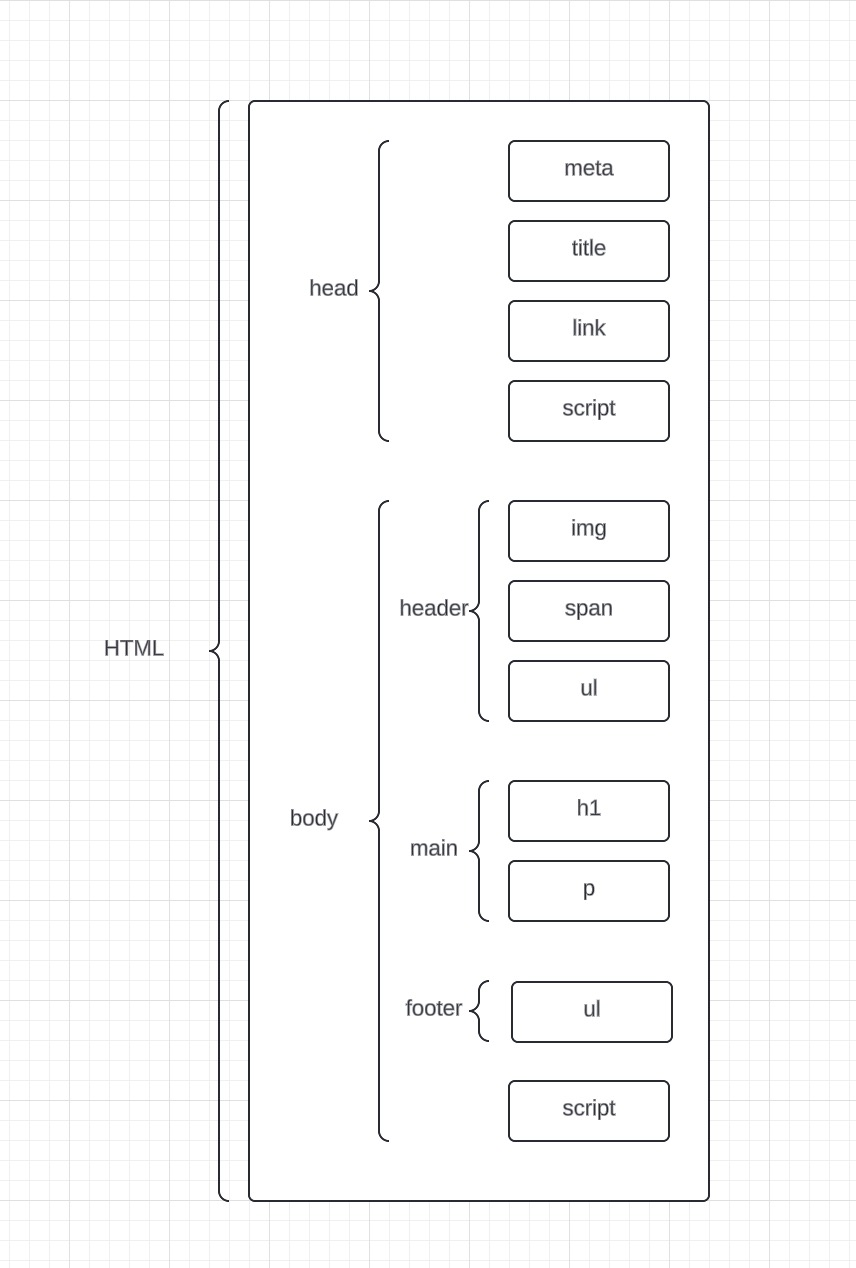
\includegraphics[width=\textwidth, height=0.3\textheight, keepaspectratio]{htmlFotos/MEindex.png}
    \caption{a) Interfaz de index.html b) Prototipo de interfaz de index.html c) Mapa de etiquetas de index.html}
    \label{fig:imagenes_conjuntas}
\end{figure}

\newpage

\subsubsection*{mapa.html}

En esta página se muestra un mapa interactivo que permite al usuario acceder a las distintas batallas de la historia. Para simplificar la visualización, se omite la parte del header y del footer, pues es la msima para todas las páginas.

\begin{figure}[H]
    \centering
    % Primera imagen (izquierda)
    \begin{minipage}{0.49\textwidth}
        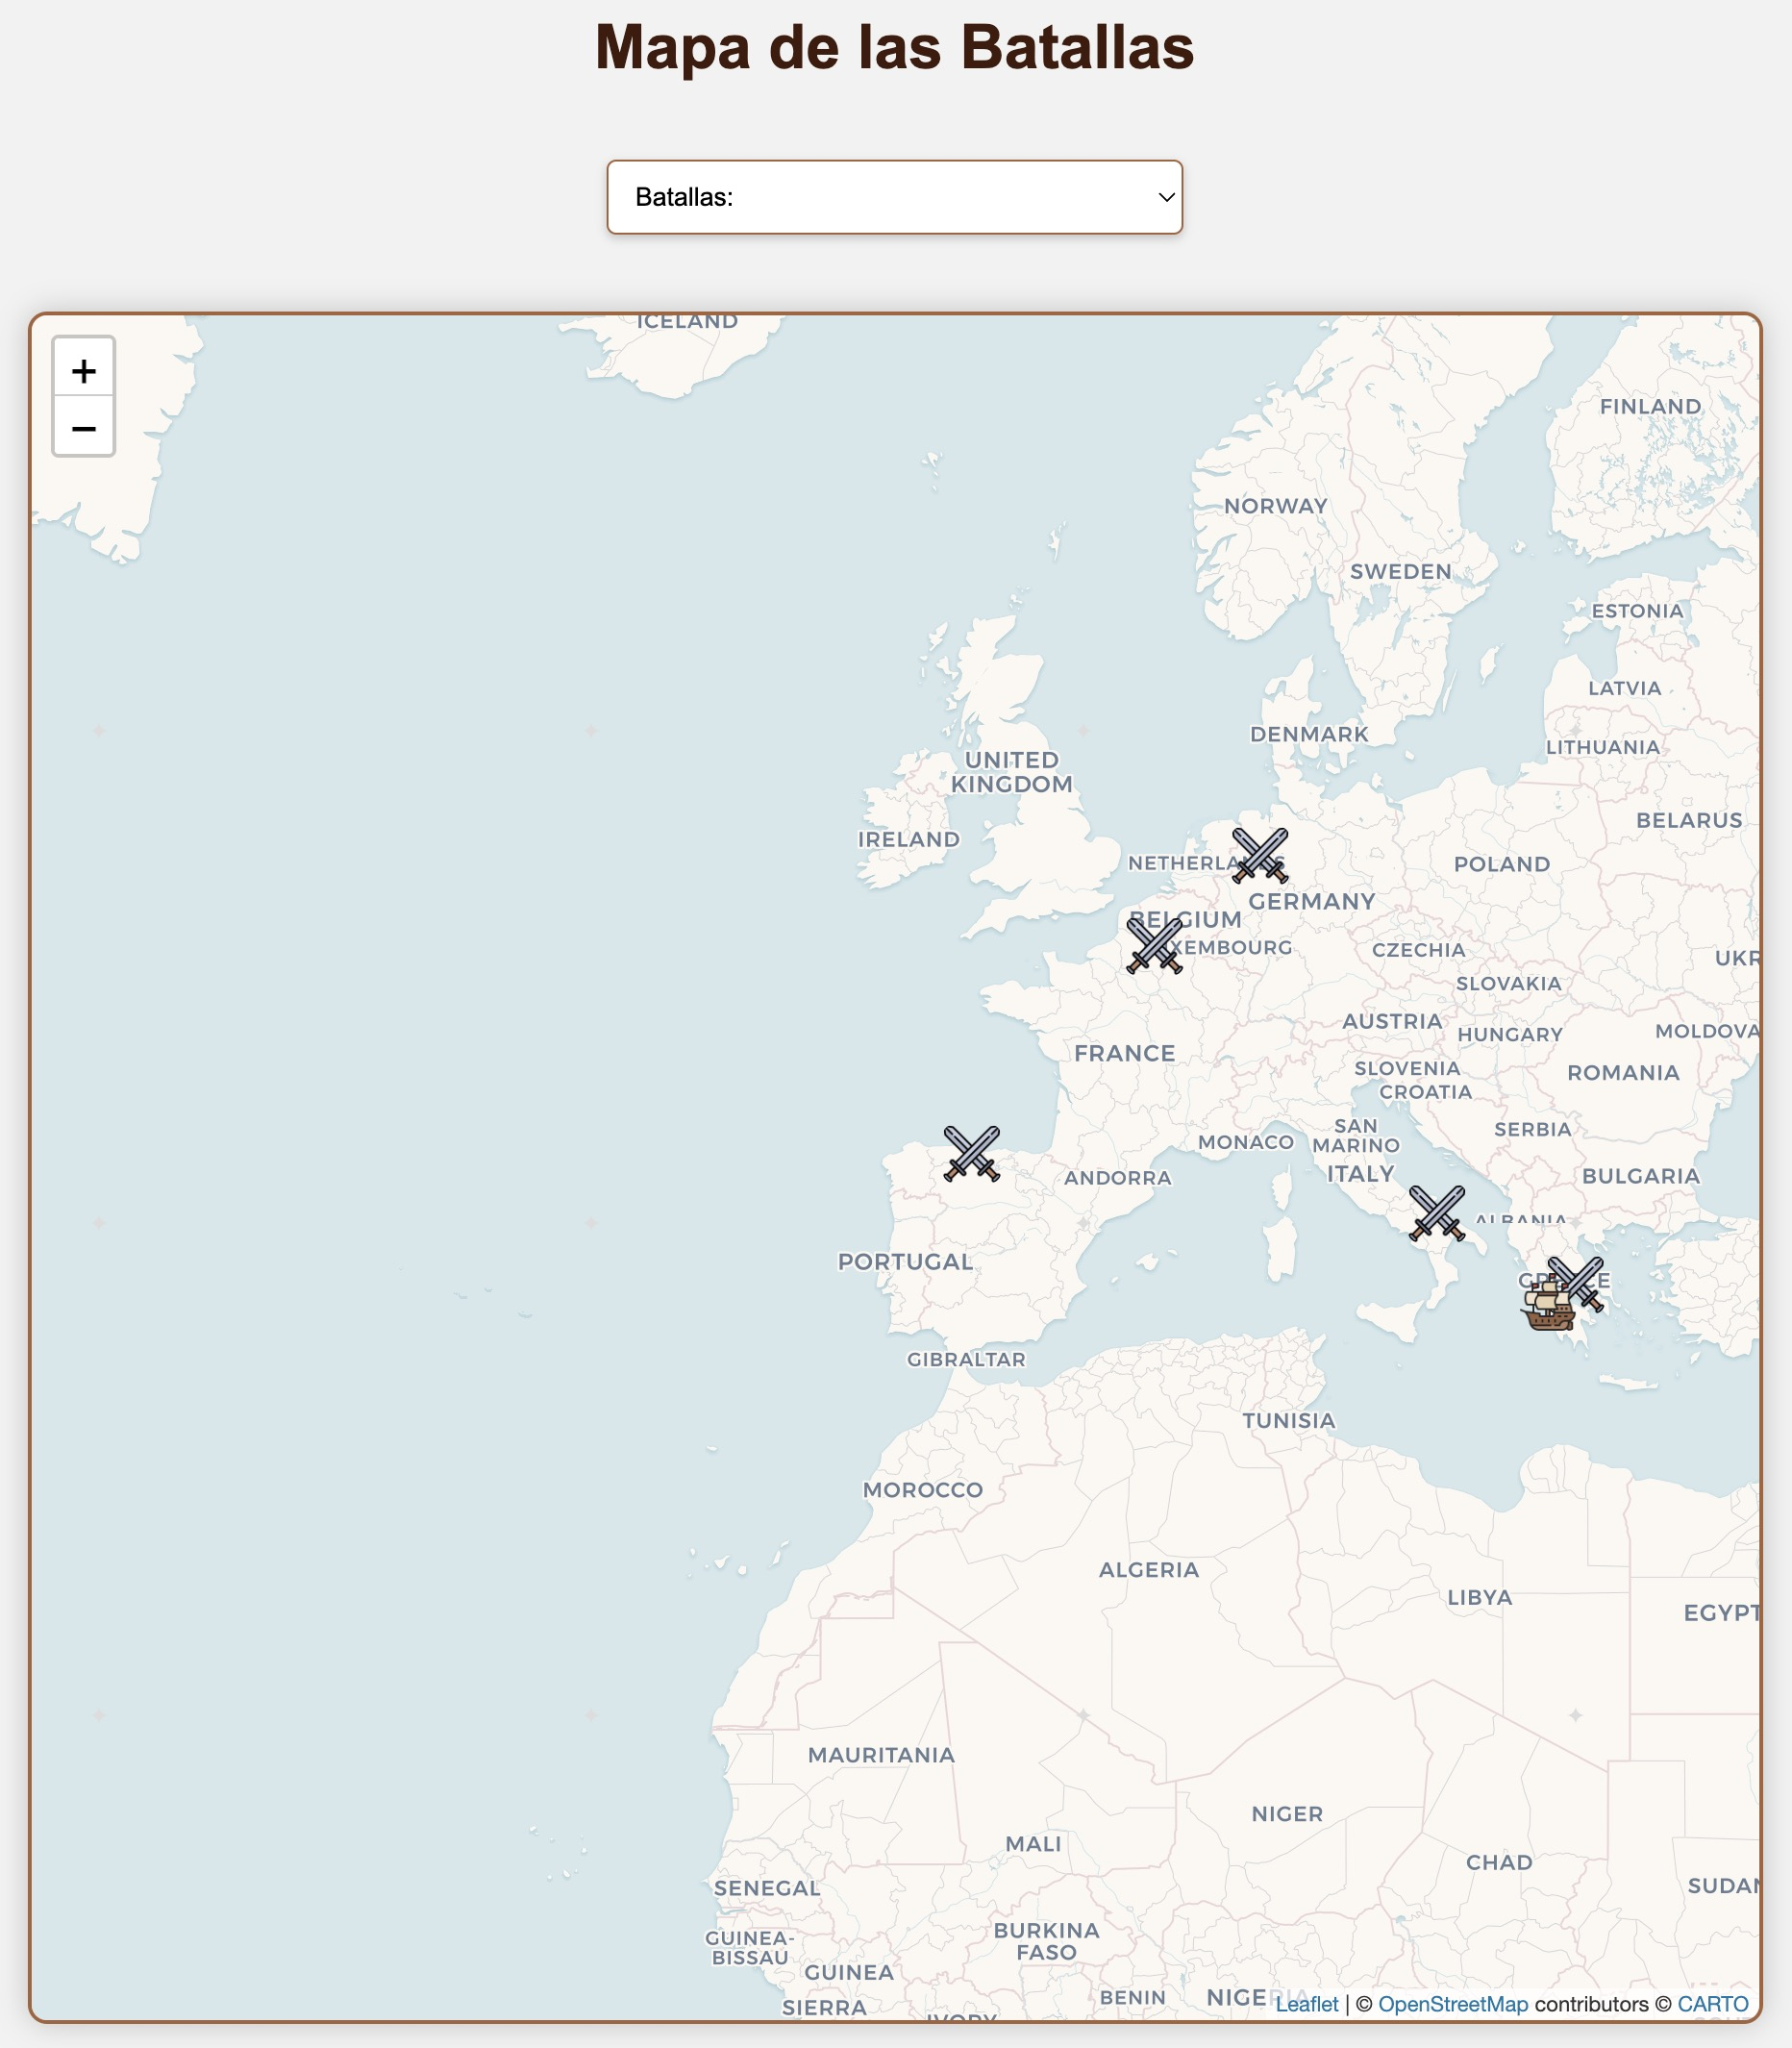
\includegraphics[width=\linewidth]{htmlFotos/mapa.jpg}
    \end{minipage}\hfill
    % Segunda imagen (derecha)
    \begin{minipage}{0.49\textwidth}
        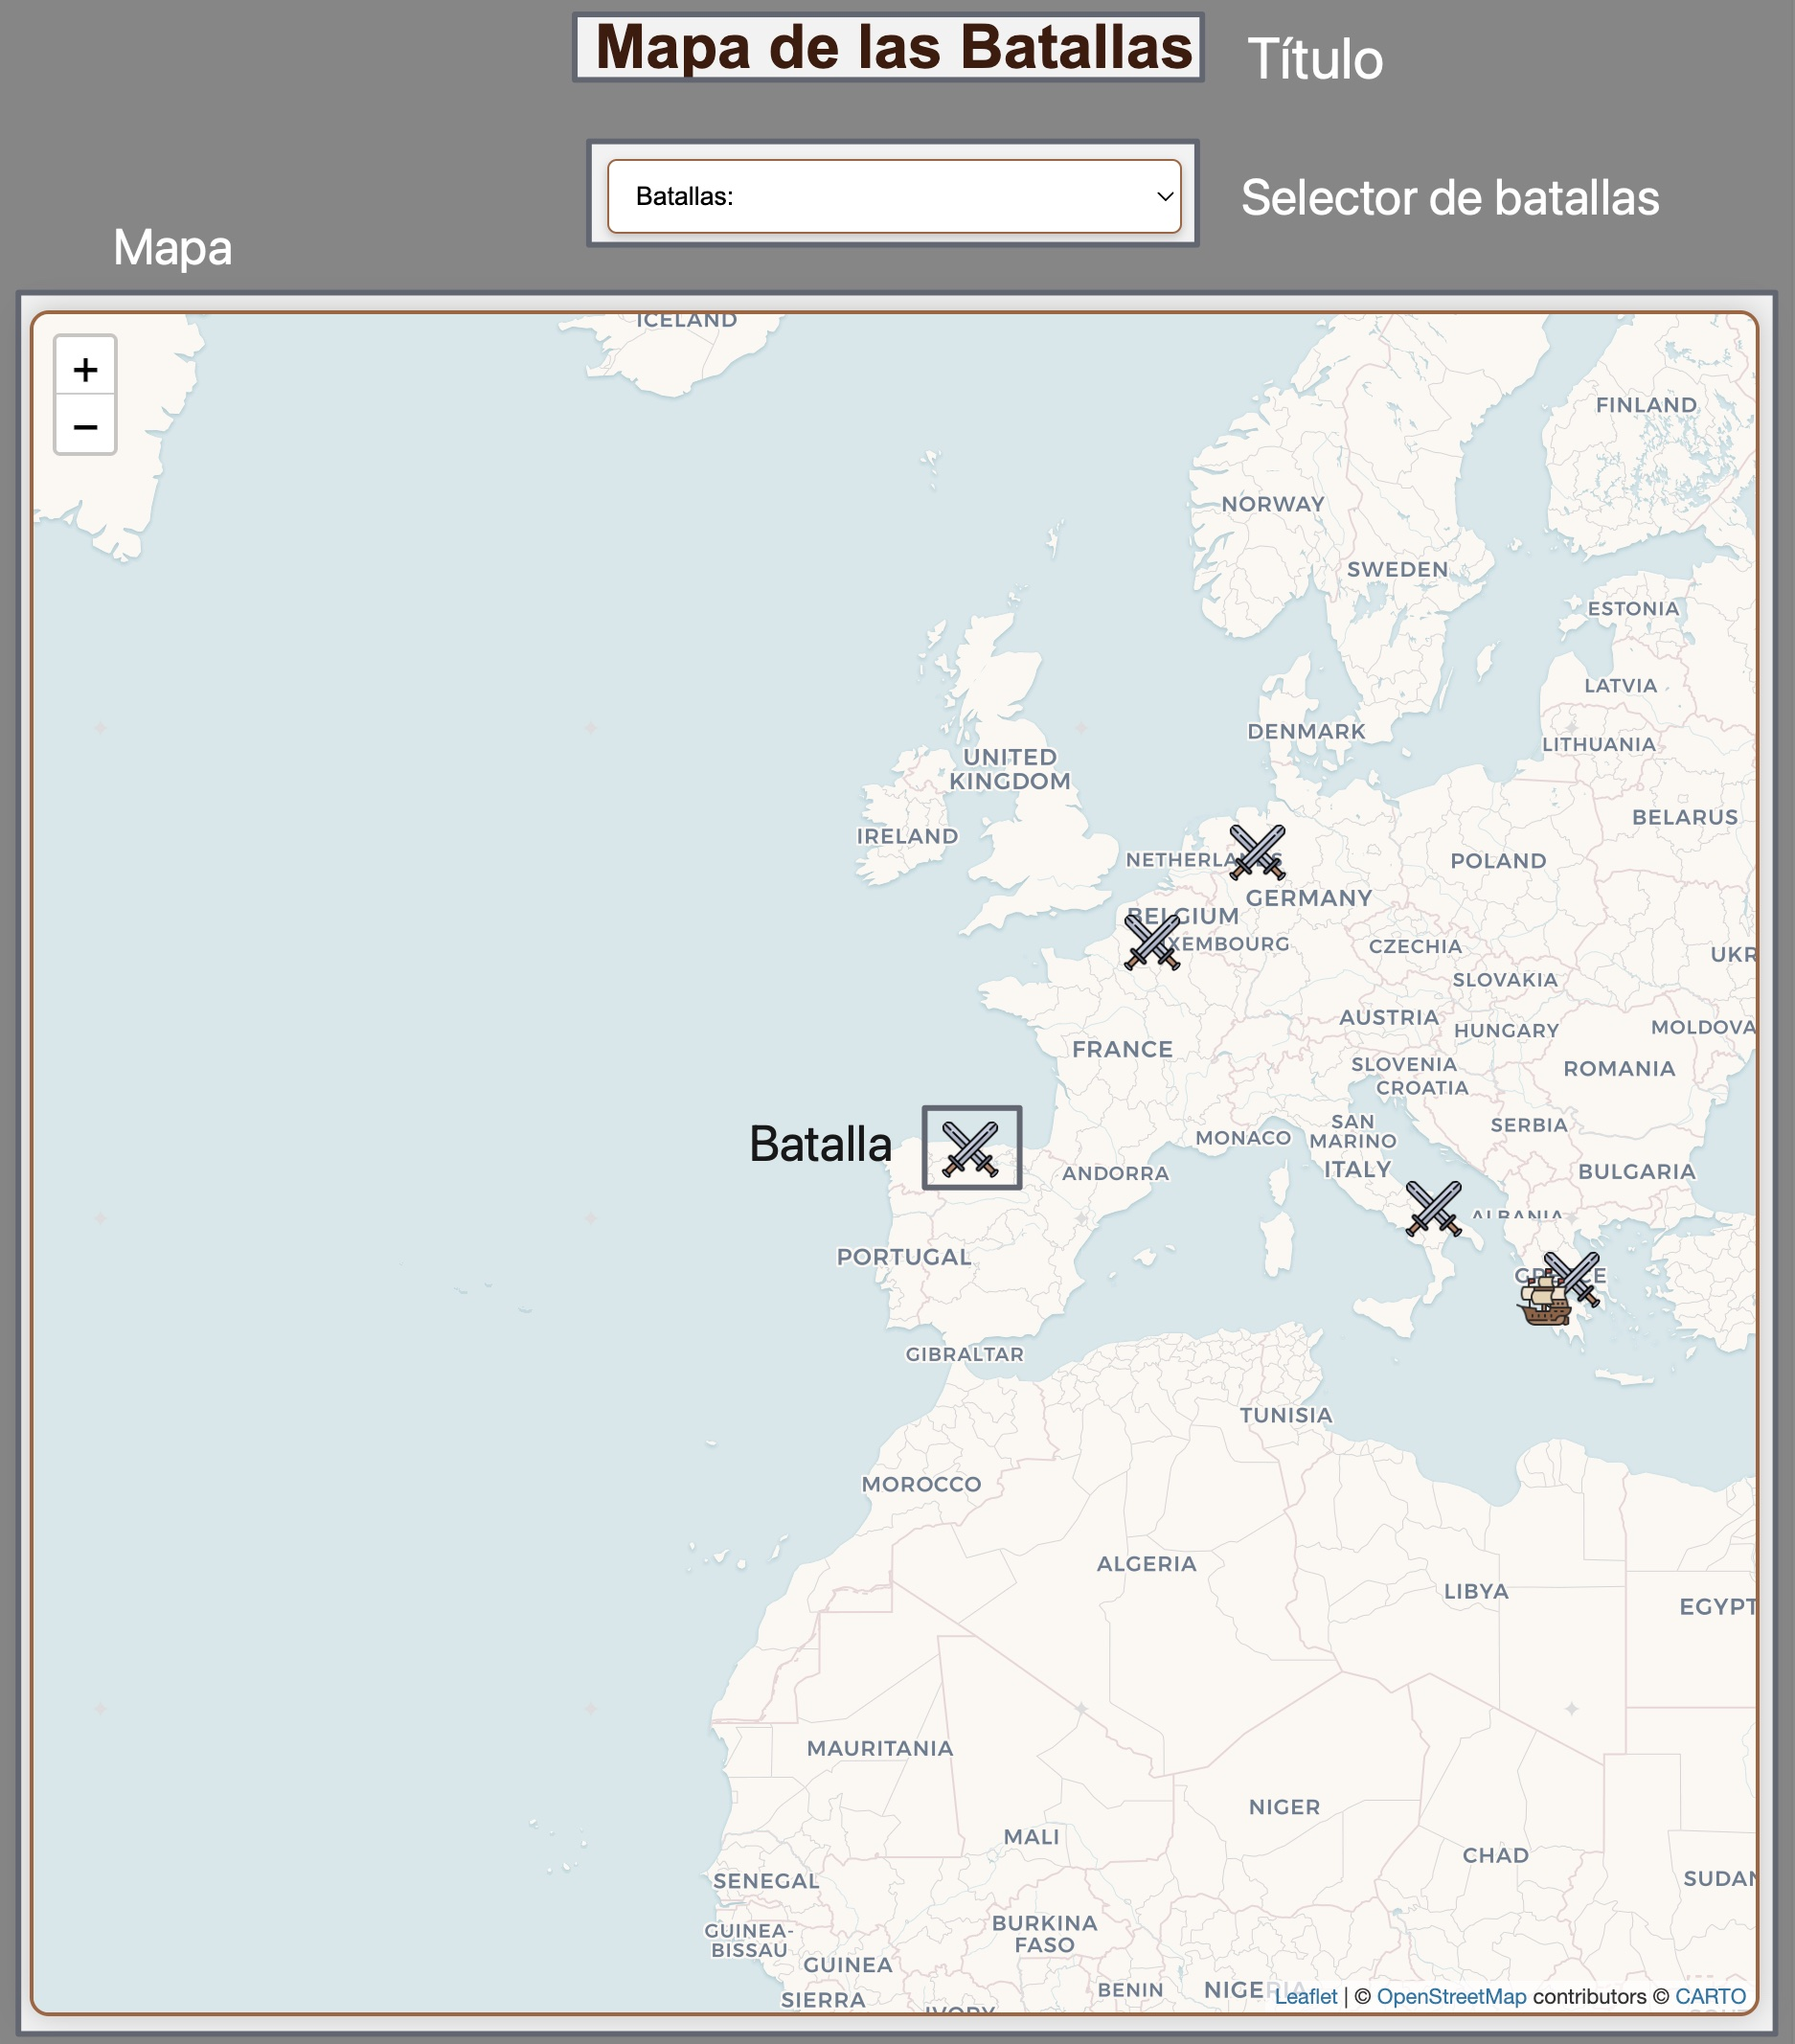
\includegraphics[width=\linewidth]{htmlFotos/prototipoMapa.jpg}
    \end{minipage}
    
    % Ajuste de espacio vertical si es necesario
    \vspace{5mm}
    
    % Tercera imagen (debajo)
    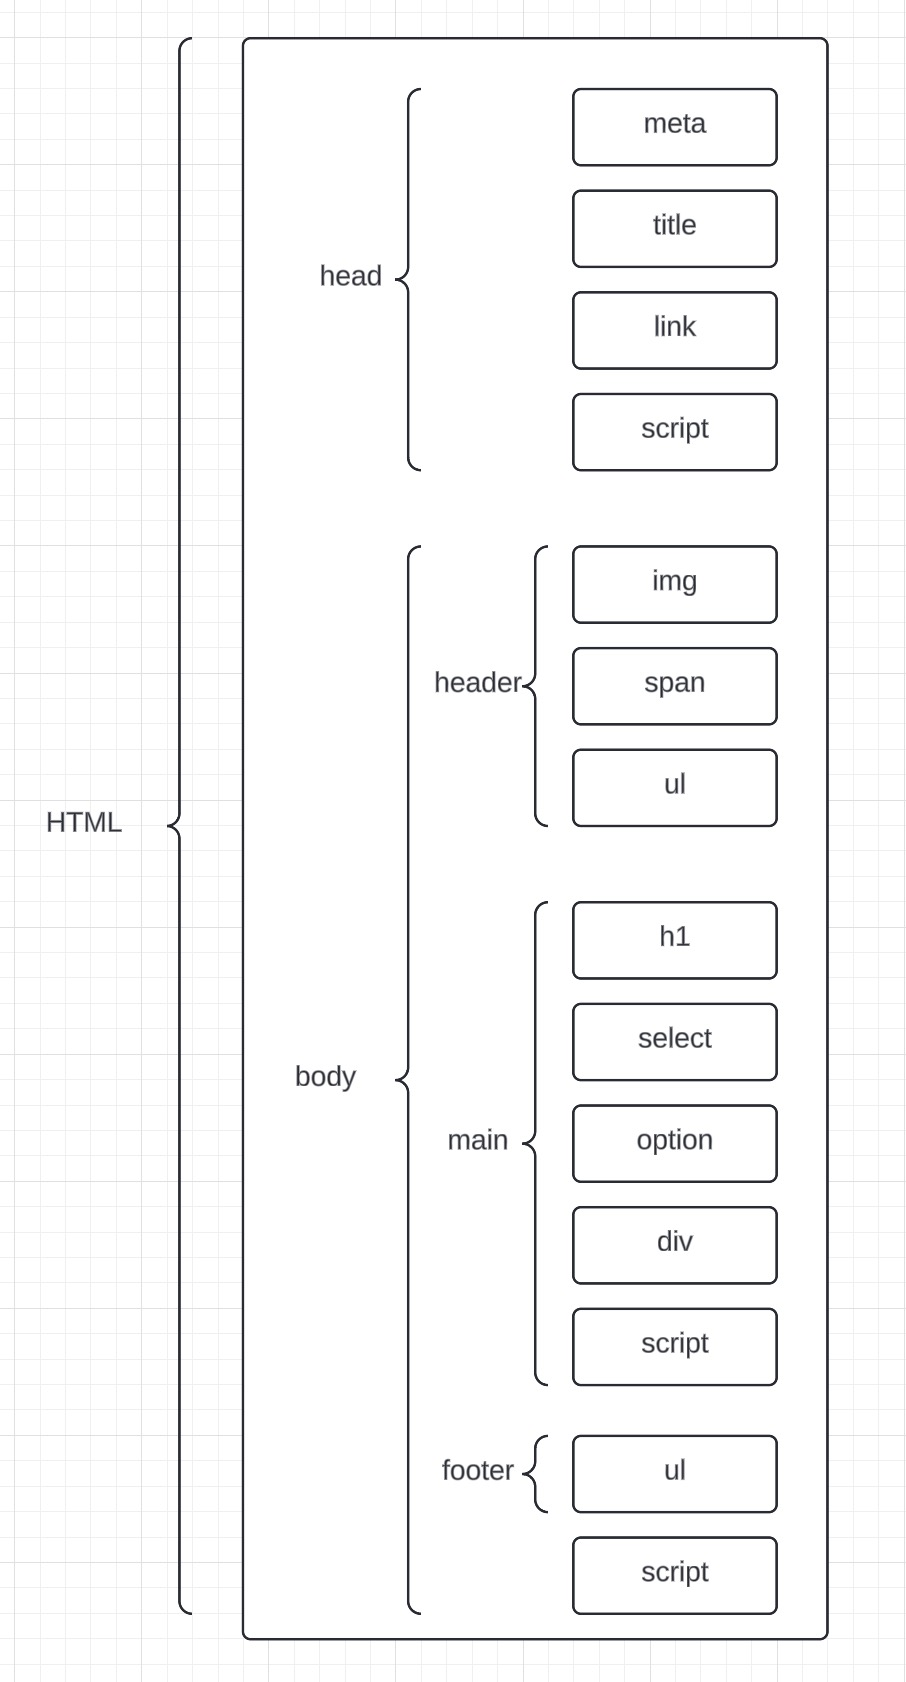
\includegraphics[width=\textwidth, height=0.4\textheight, keepaspectratio]{htmlFotos/MEmapa.jpg}
    \caption{a) Interfaz de AH.html b) Prototipo de interfaz de AH.html c) Mapa de etiquetas de AH.html}
    \label{fig:imagenes_conjuntas}
\end{figure}

\newpage

\subsubsection*{AH.html, batallas.html, guerras.html y personajesEmblematicos.html}

Para ver como se descomponen estas secciones de nuestra web, tomaremos como ejemplo la página de Acontecimientos Históricos, aunque las otras páginas siguen un esquema similar. Como en el caso anterior, se omite la parte del header y del footer, pues es la misma para todas las páginas.

\begin{figure}[H]
    \centering
    % Primera imagen (izquierda)
    \begin{minipage}{0.49\textwidth}
        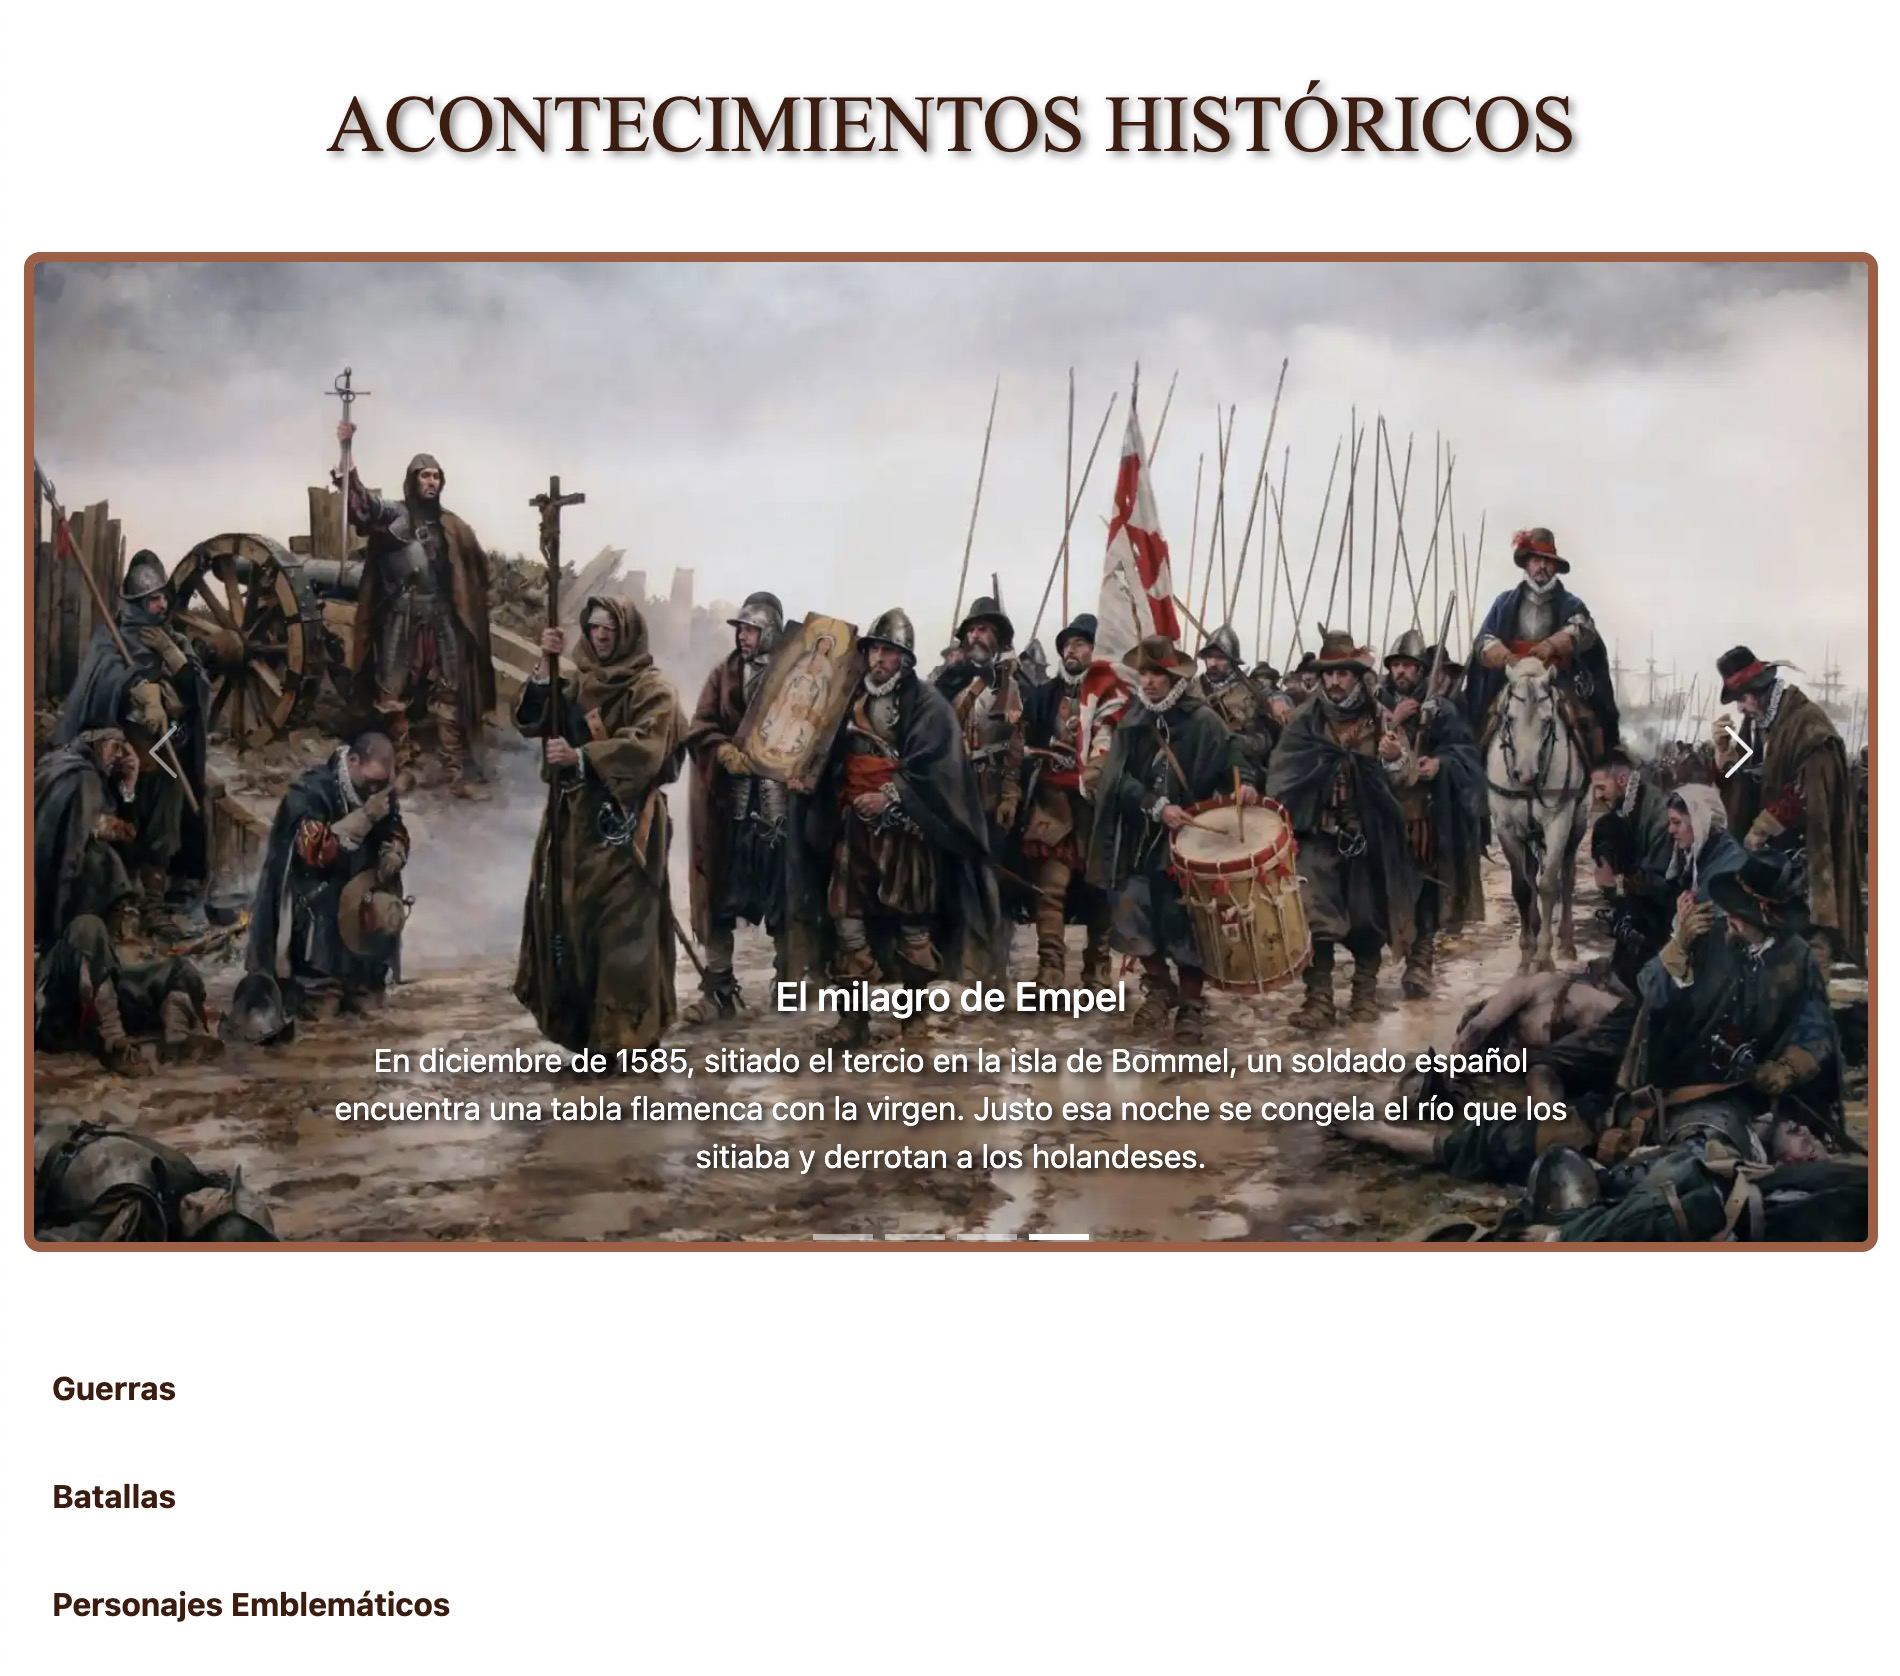
\includegraphics[width=\linewidth]{htmlFotos/AH.jpg}
    \end{minipage}\hfill
    % Segunda imagen (derecha)
    \begin{minipage}{0.49\textwidth}
        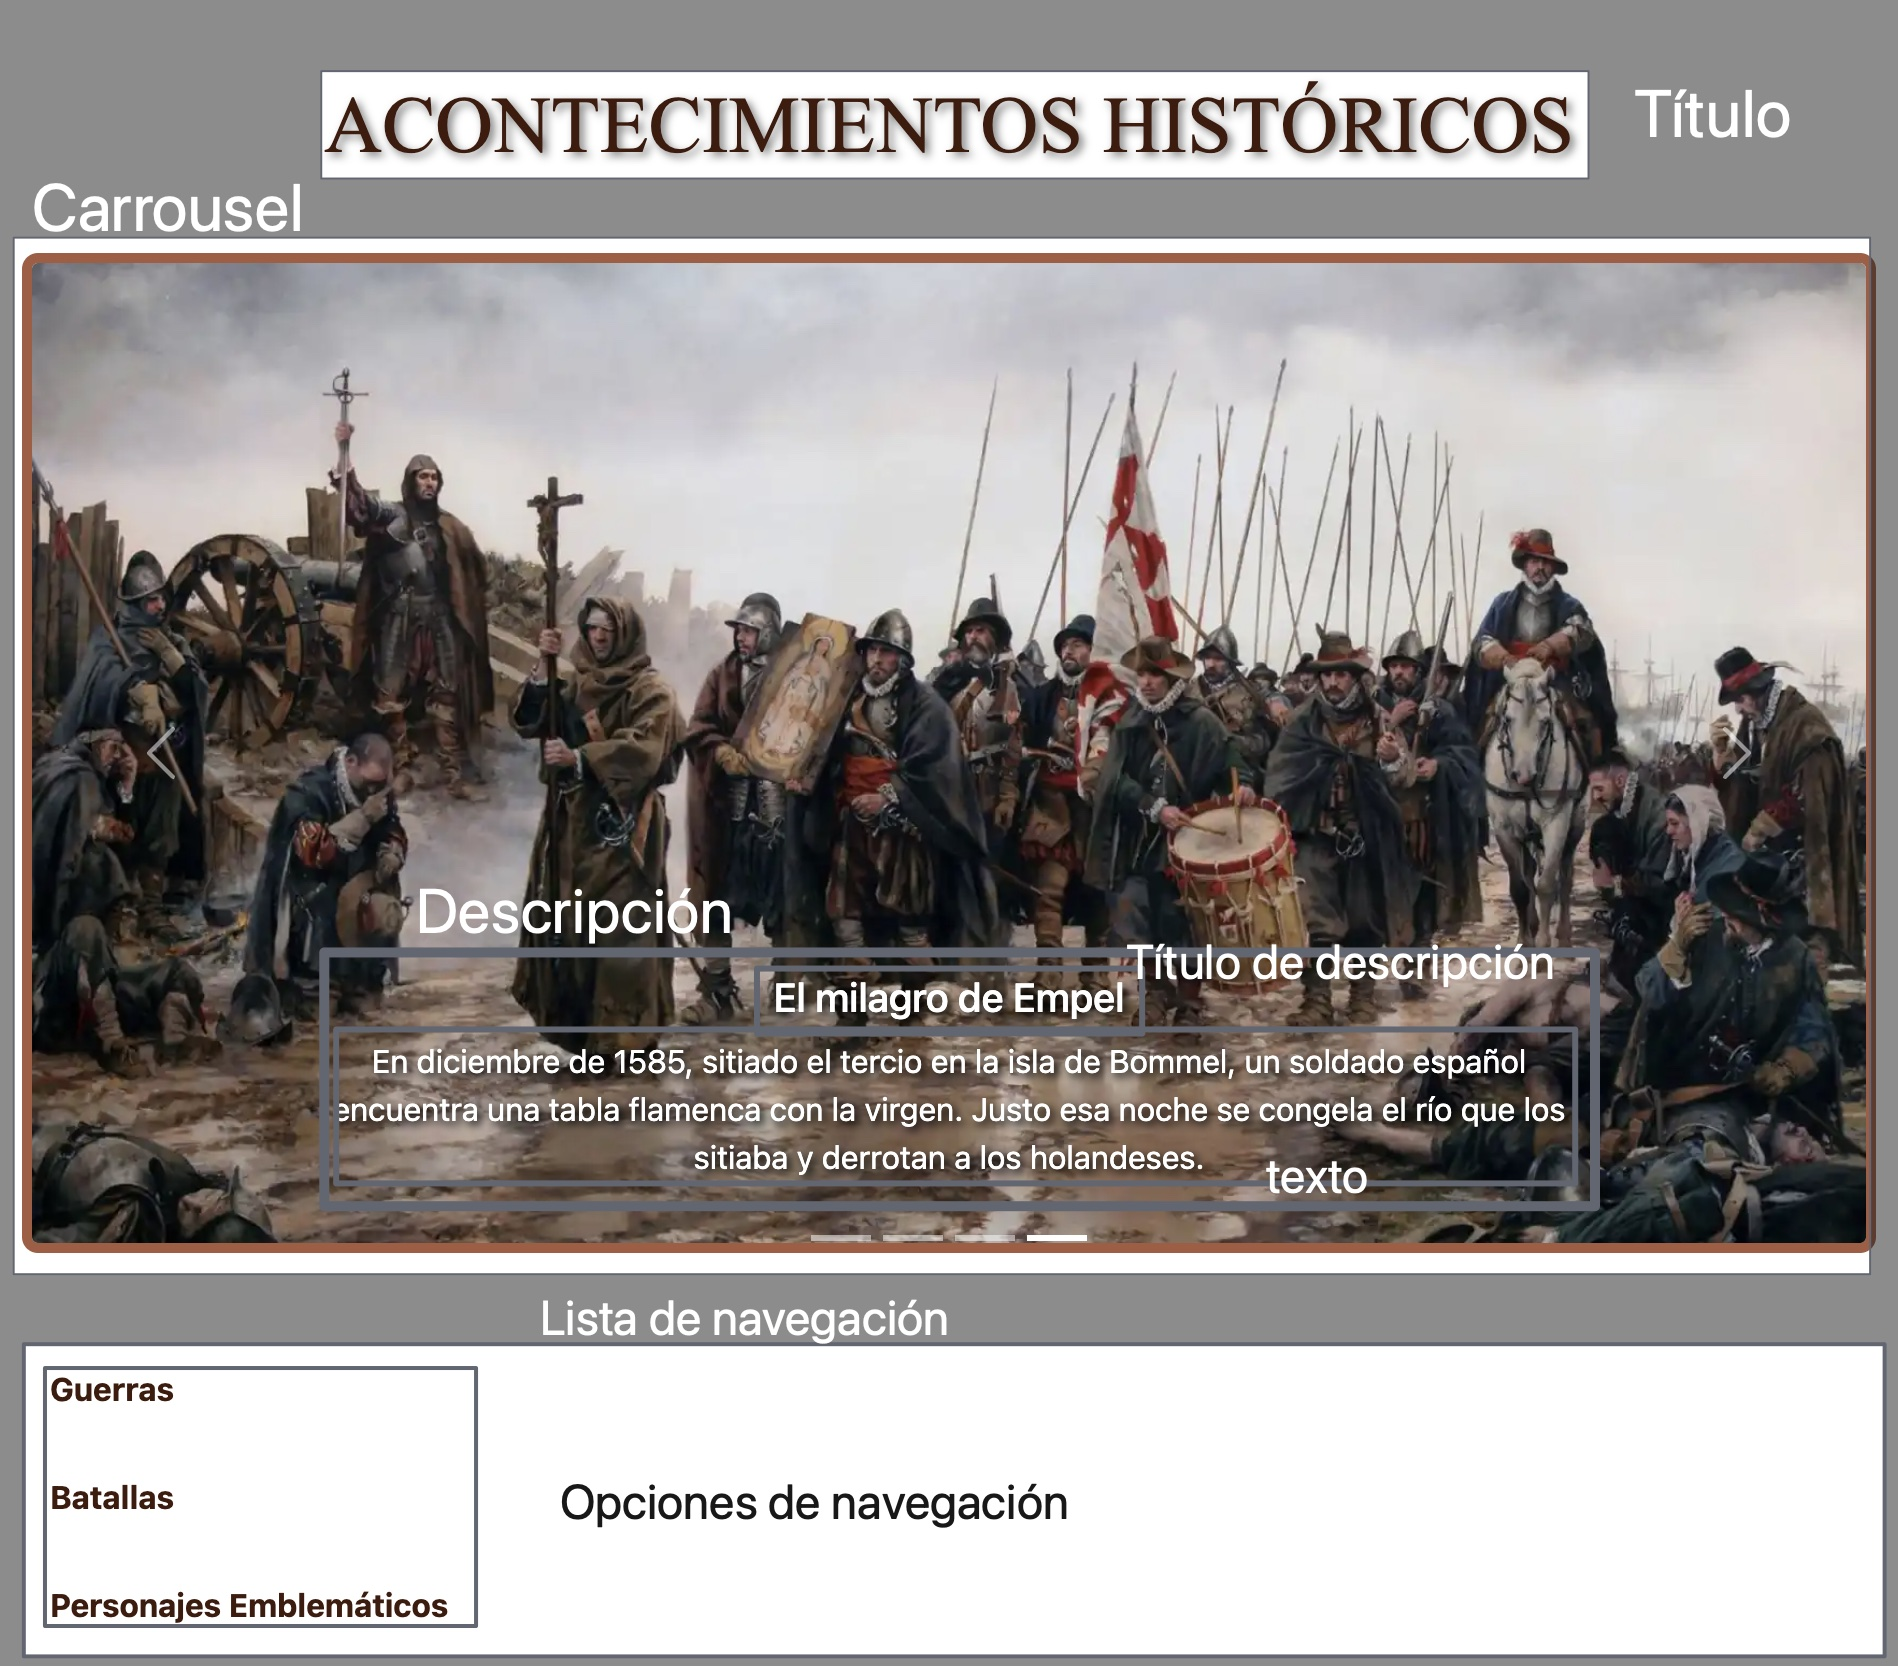
\includegraphics[width=\linewidth]{htmlFotos/prototipoAH.jpg}
    \end{minipage}
    
    % Ajuste de espacio vertical si es necesario
    \vspace{5mm}
    
    % Tercera imagen (debajo)
    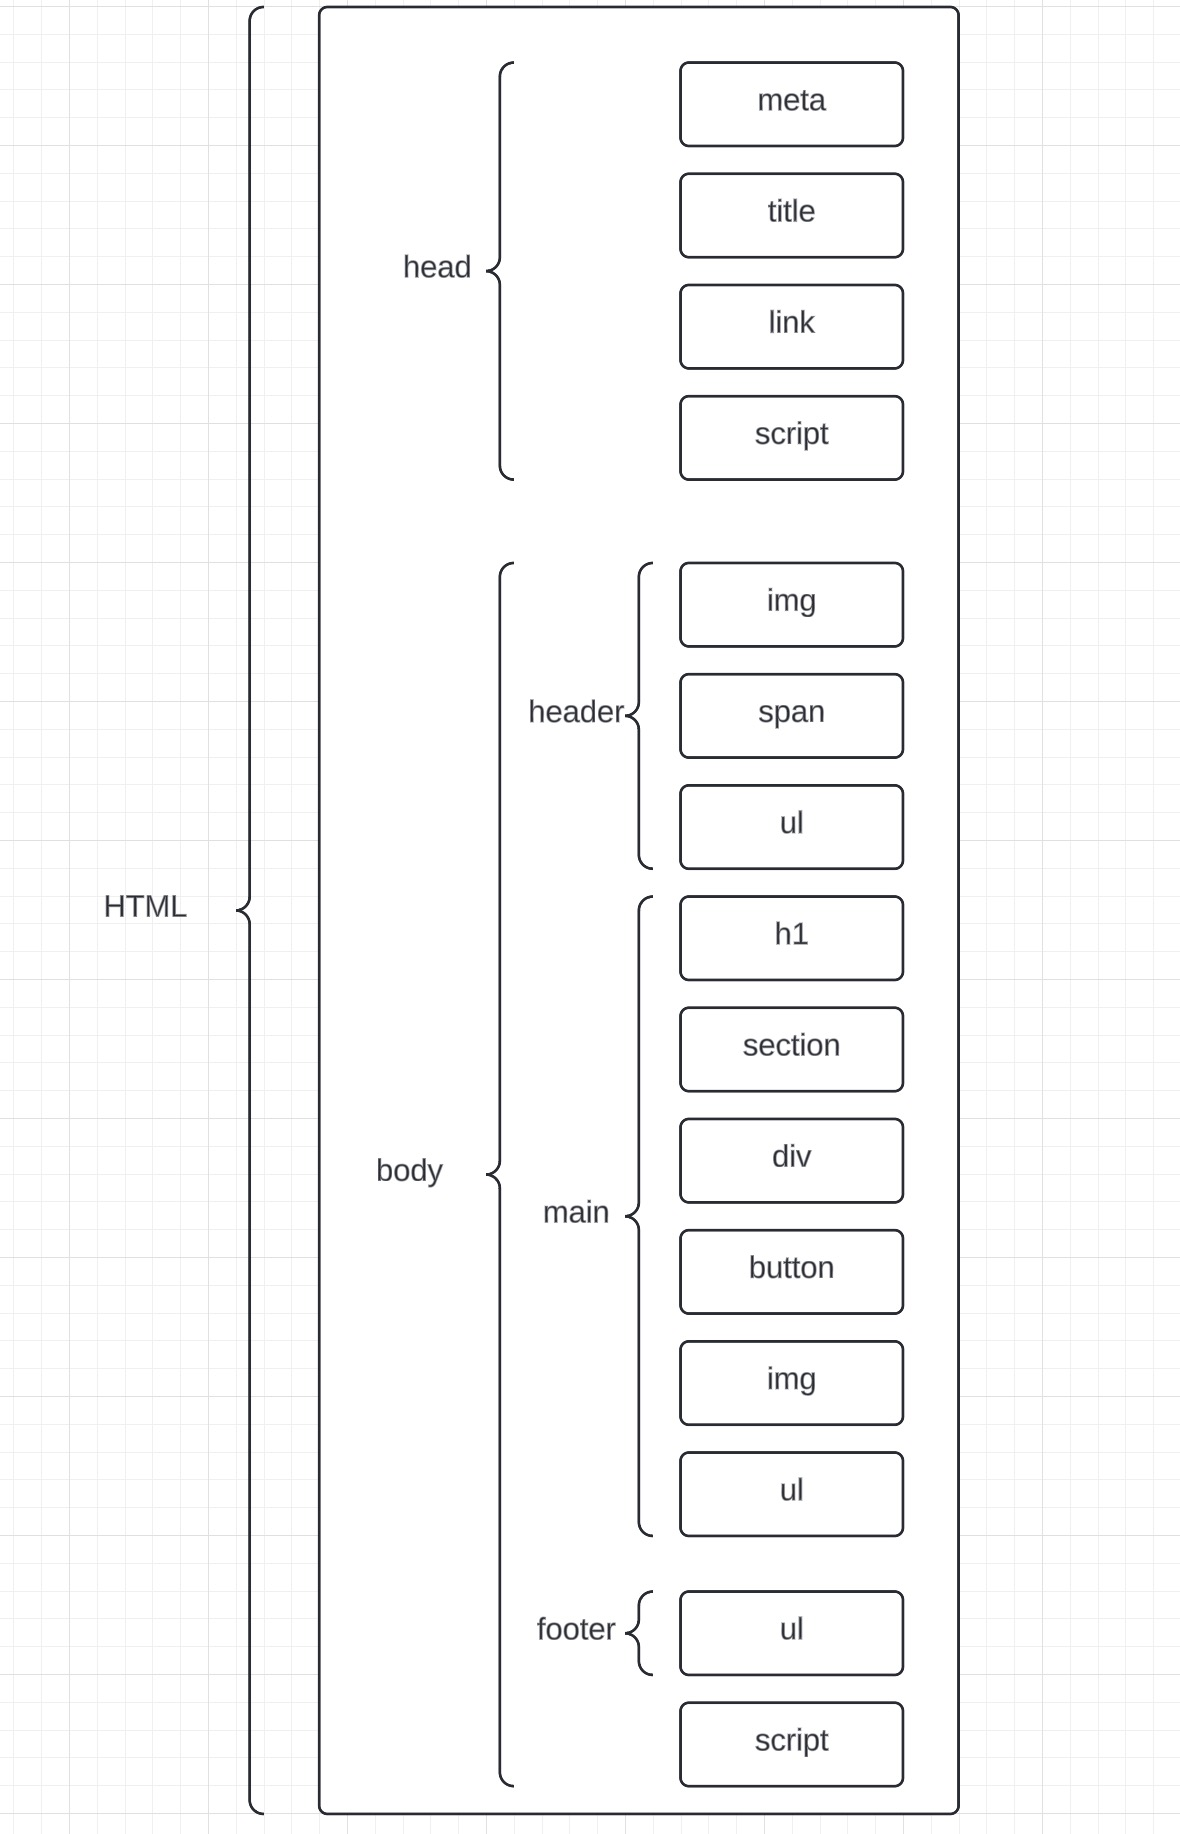
\includegraphics[width=\textwidth, height=0.5\textheight, keepaspectratio]{htmlFotos/MEAH.jpg}
    \caption{a) Interfaz de mapa.html b) Prototipo de interfaz de mapa.html c) Mapa de etiquetas de mapa.html}
    \label{fig:imagenes_conjuntas}
\end{figure}

\subsection*{LibrosEA.html, LibrosEC.html, LibrosEM.html, LibrosEMed.html}

Estas páginas son las que contienen la información de los libros recomendados para cada época histórica. A continuación se muestra la estructura de la página de libros de la Edad moderna, aunque las demás páginas siguen un esquema similar. Nos abstendremos, de nuevo, de mostrar la parte del header y del footer.

\begin{figure}[H]
    \centering
    % Primera imagen (izquierda)
    \begin{minipage}{0.49\textwidth}
        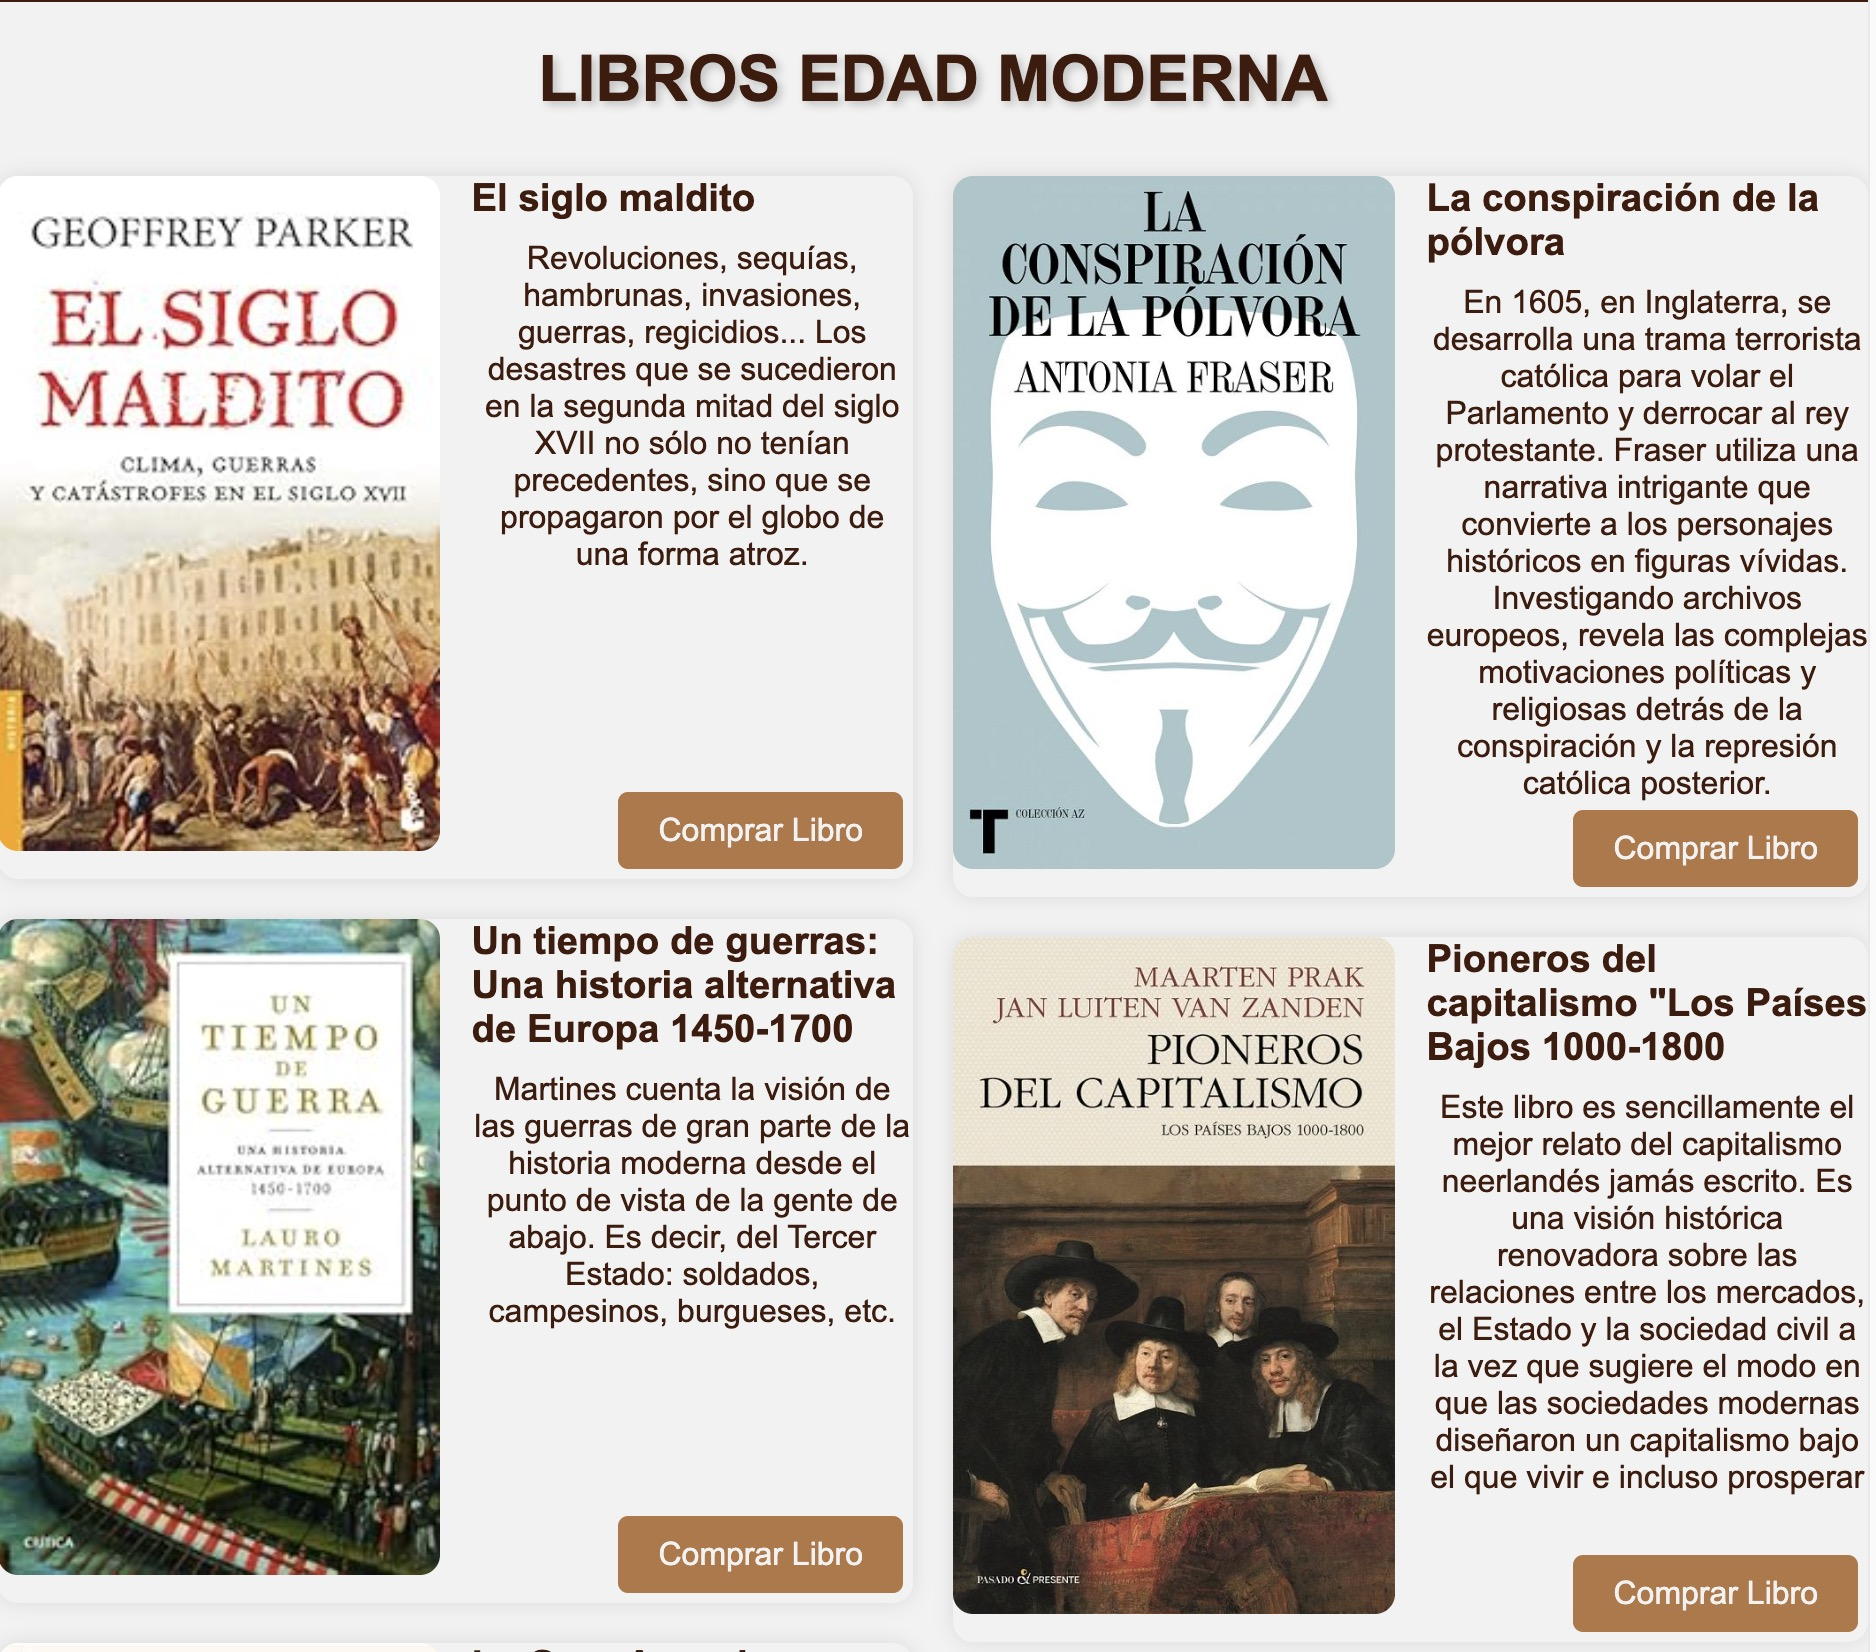
\includegraphics[width=\linewidth]{htmlFotos/libros.jpg}
    \end{minipage}\hfill
    % Segunda imagen (derecha)
    \begin{minipage}{0.49\textwidth}
        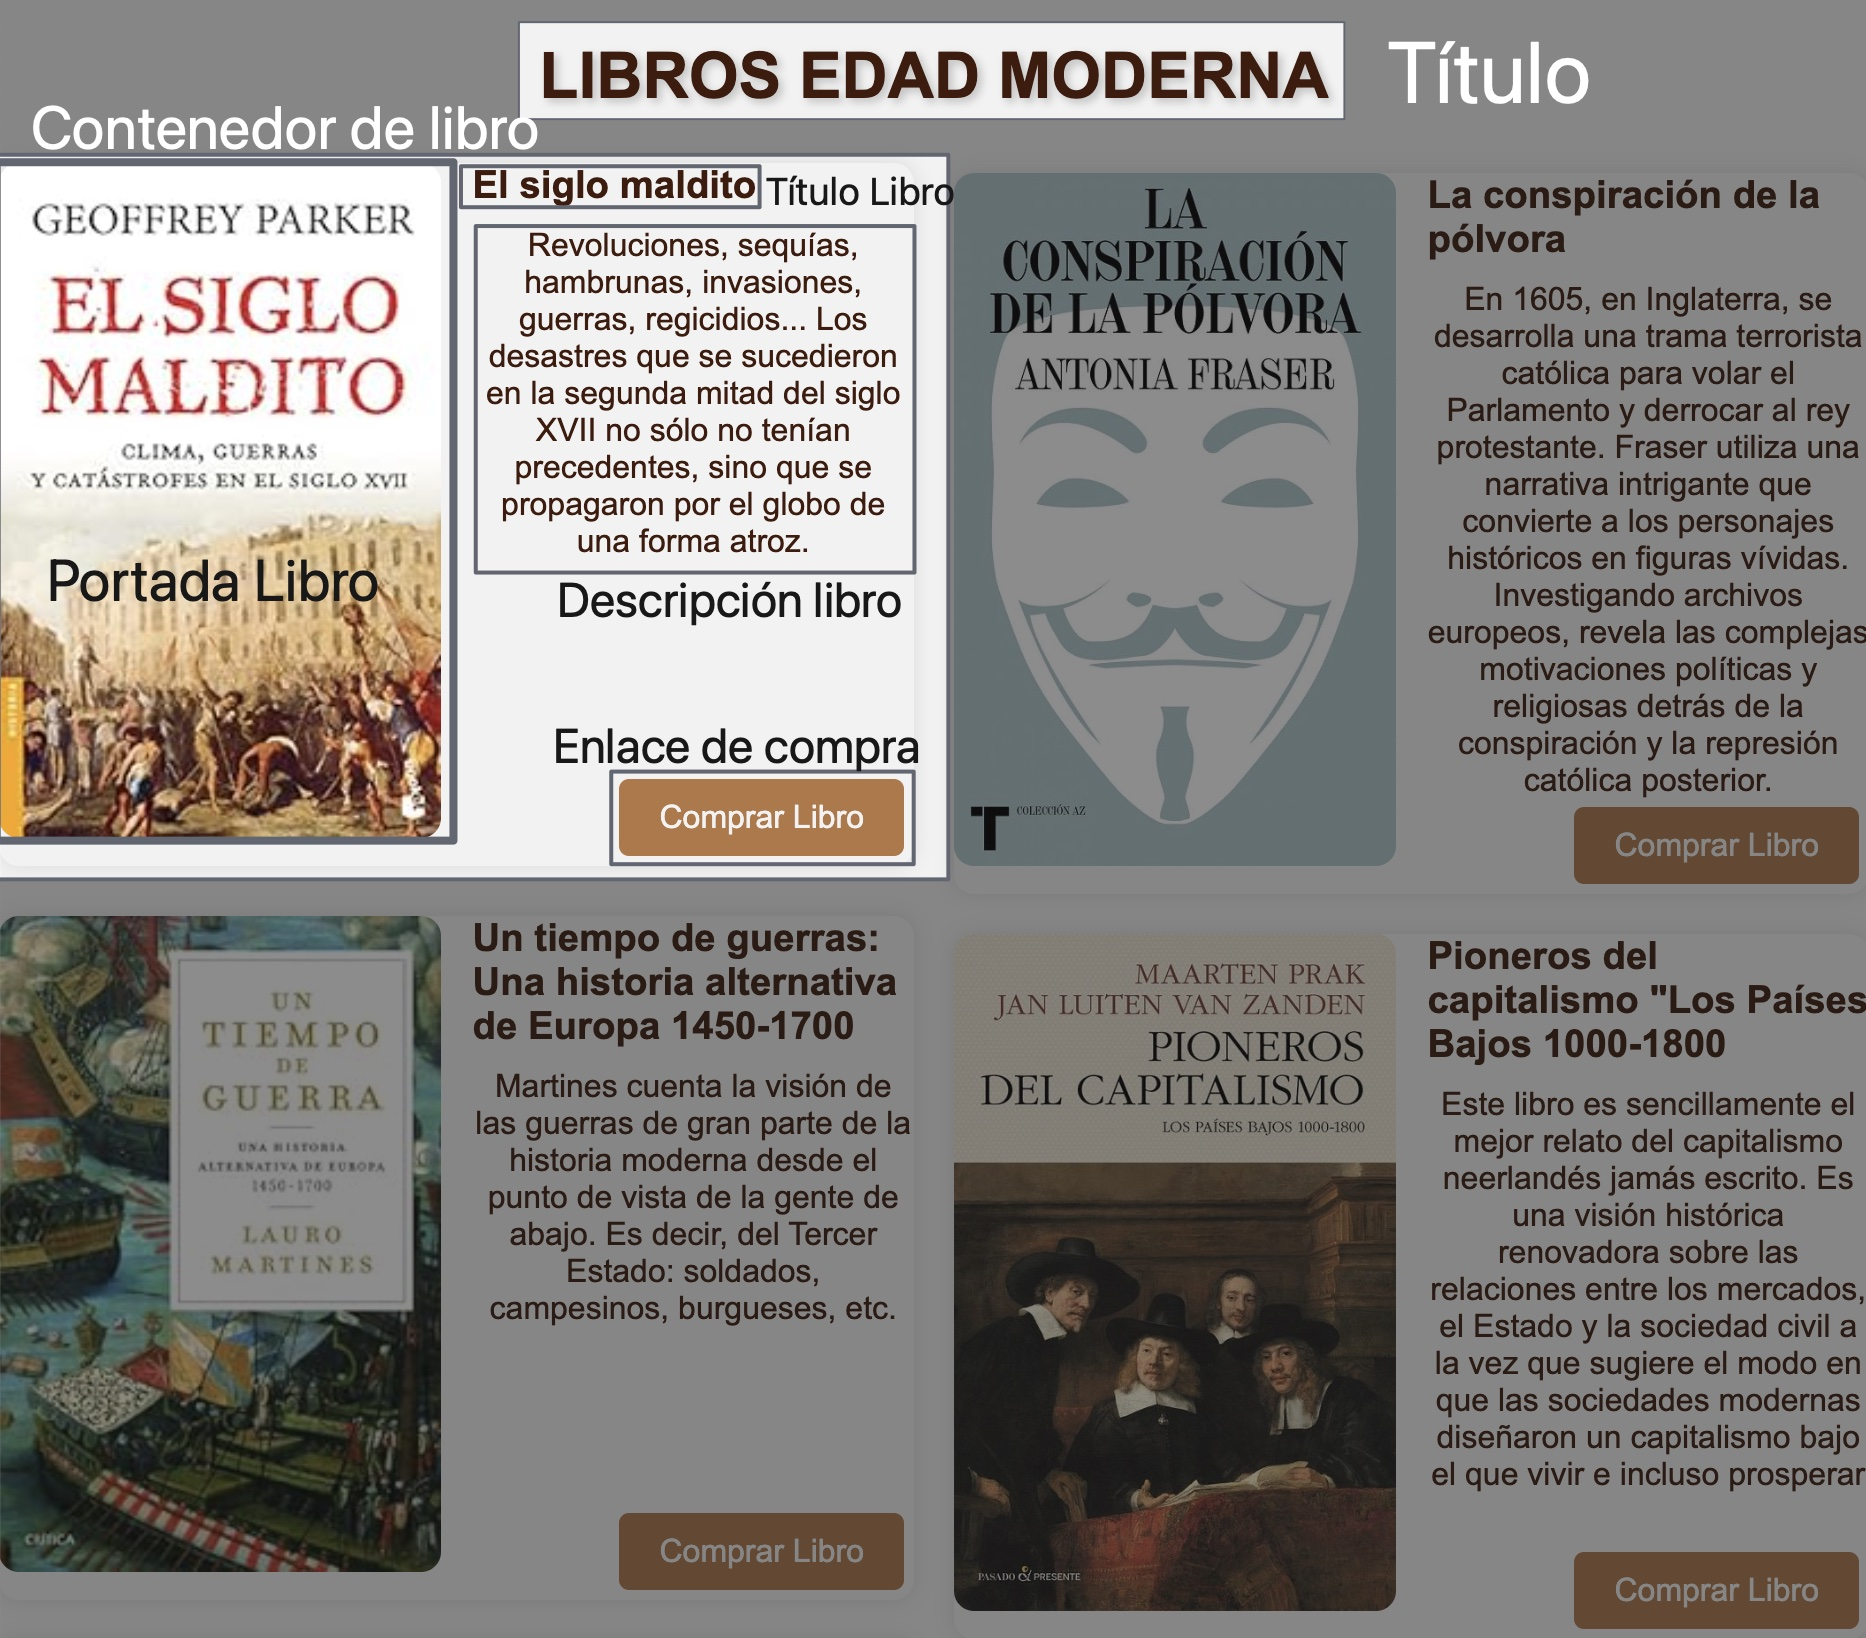
\includegraphics[width=\linewidth]{htmlFotos/prototipoLibros.jpg}
    \end{minipage}
    
    % Ajuste de espacio vertical si es necesario
    \vspace{5mm}
    
    % Tercera imagen (debajo)
    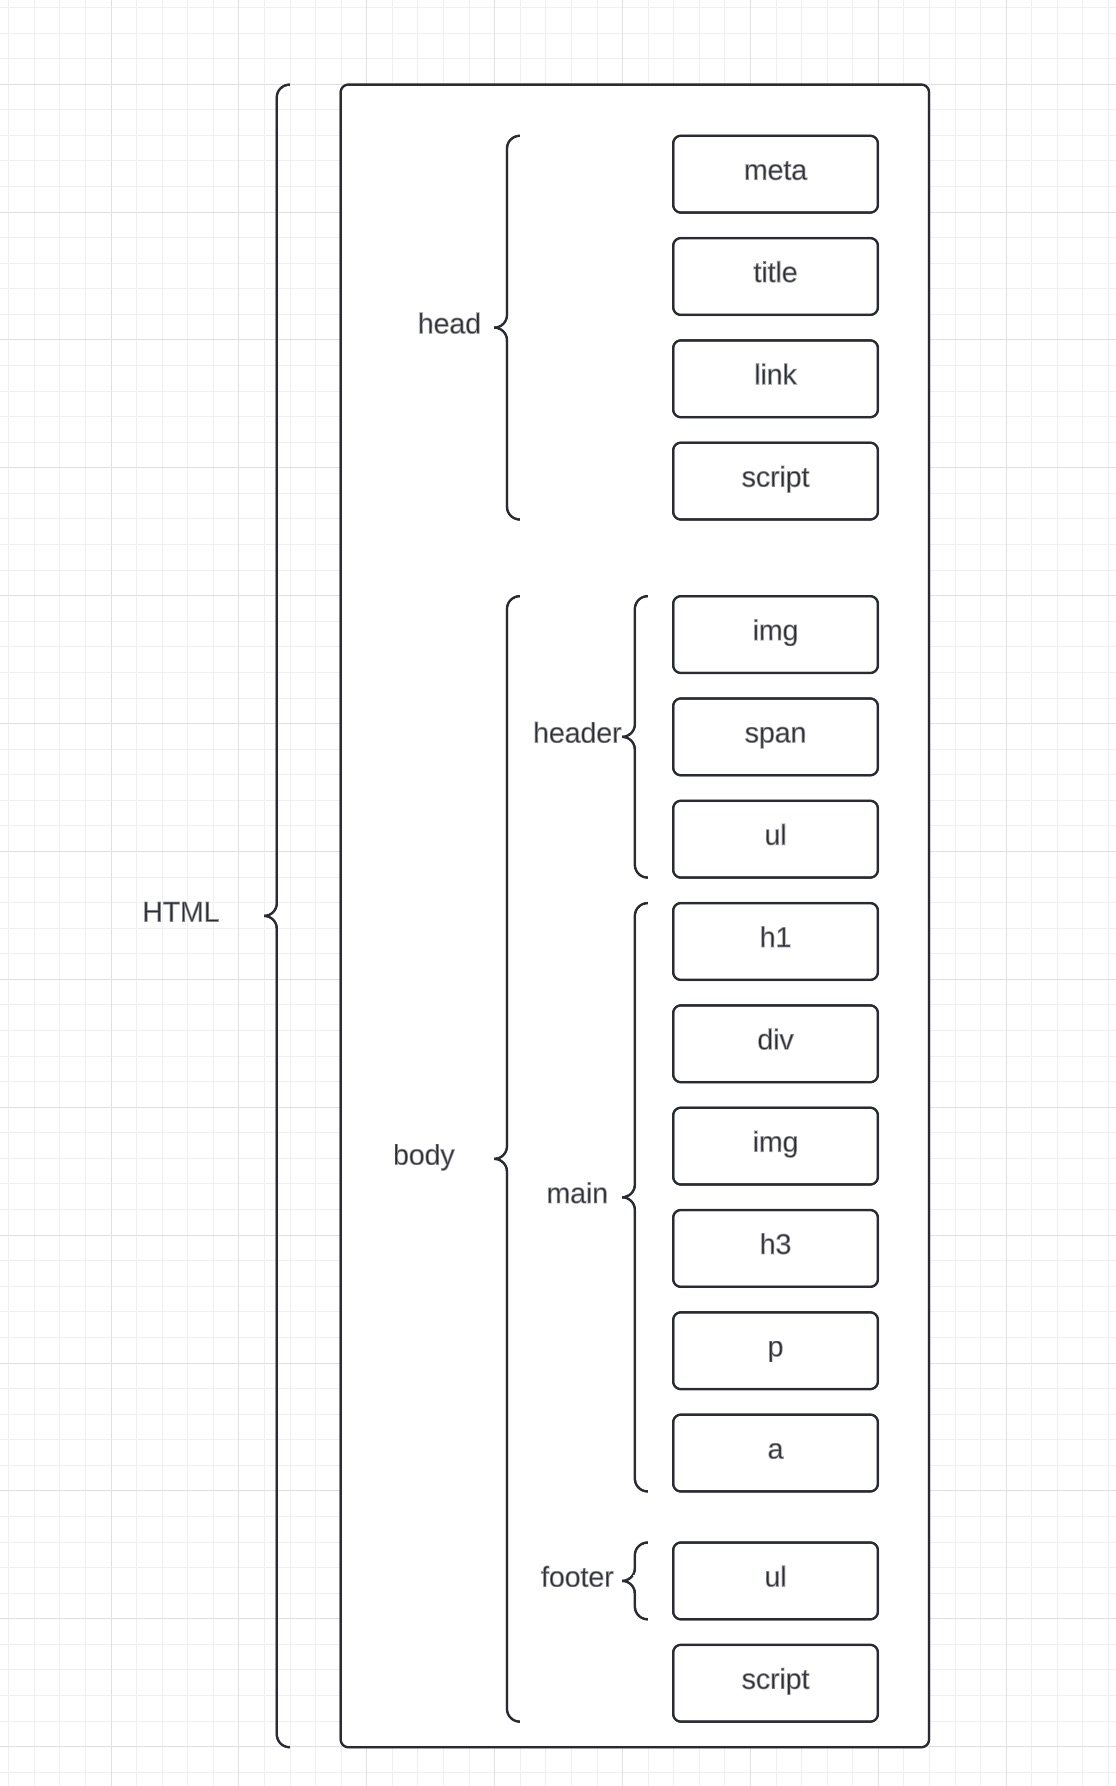
\includegraphics[width=\textwidth, height=0.5\textheight, keepaspectratio]{htmlFotos/MElibros.jpg}
    \caption{a) Interfaz de libros.html b) Prototipo de interfaz de libros.html c) Mapa de etiquetas de libros.html}
    \label{fig:imagenes_conjuntas}
\end{figure}

\subsection*{Foro.html}

Esta página es la que contiene el foro de nuestra web, donde los usuarios pueden discutir sobre distintos temas. Los headers y footers son los mismos que en las otras páginas, por lo que no se mostrarán.


\begin{figure}[H]
    \centering
    % Primera imagen (izquierda)
    \begin{minipage}{0.49\textwidth}
        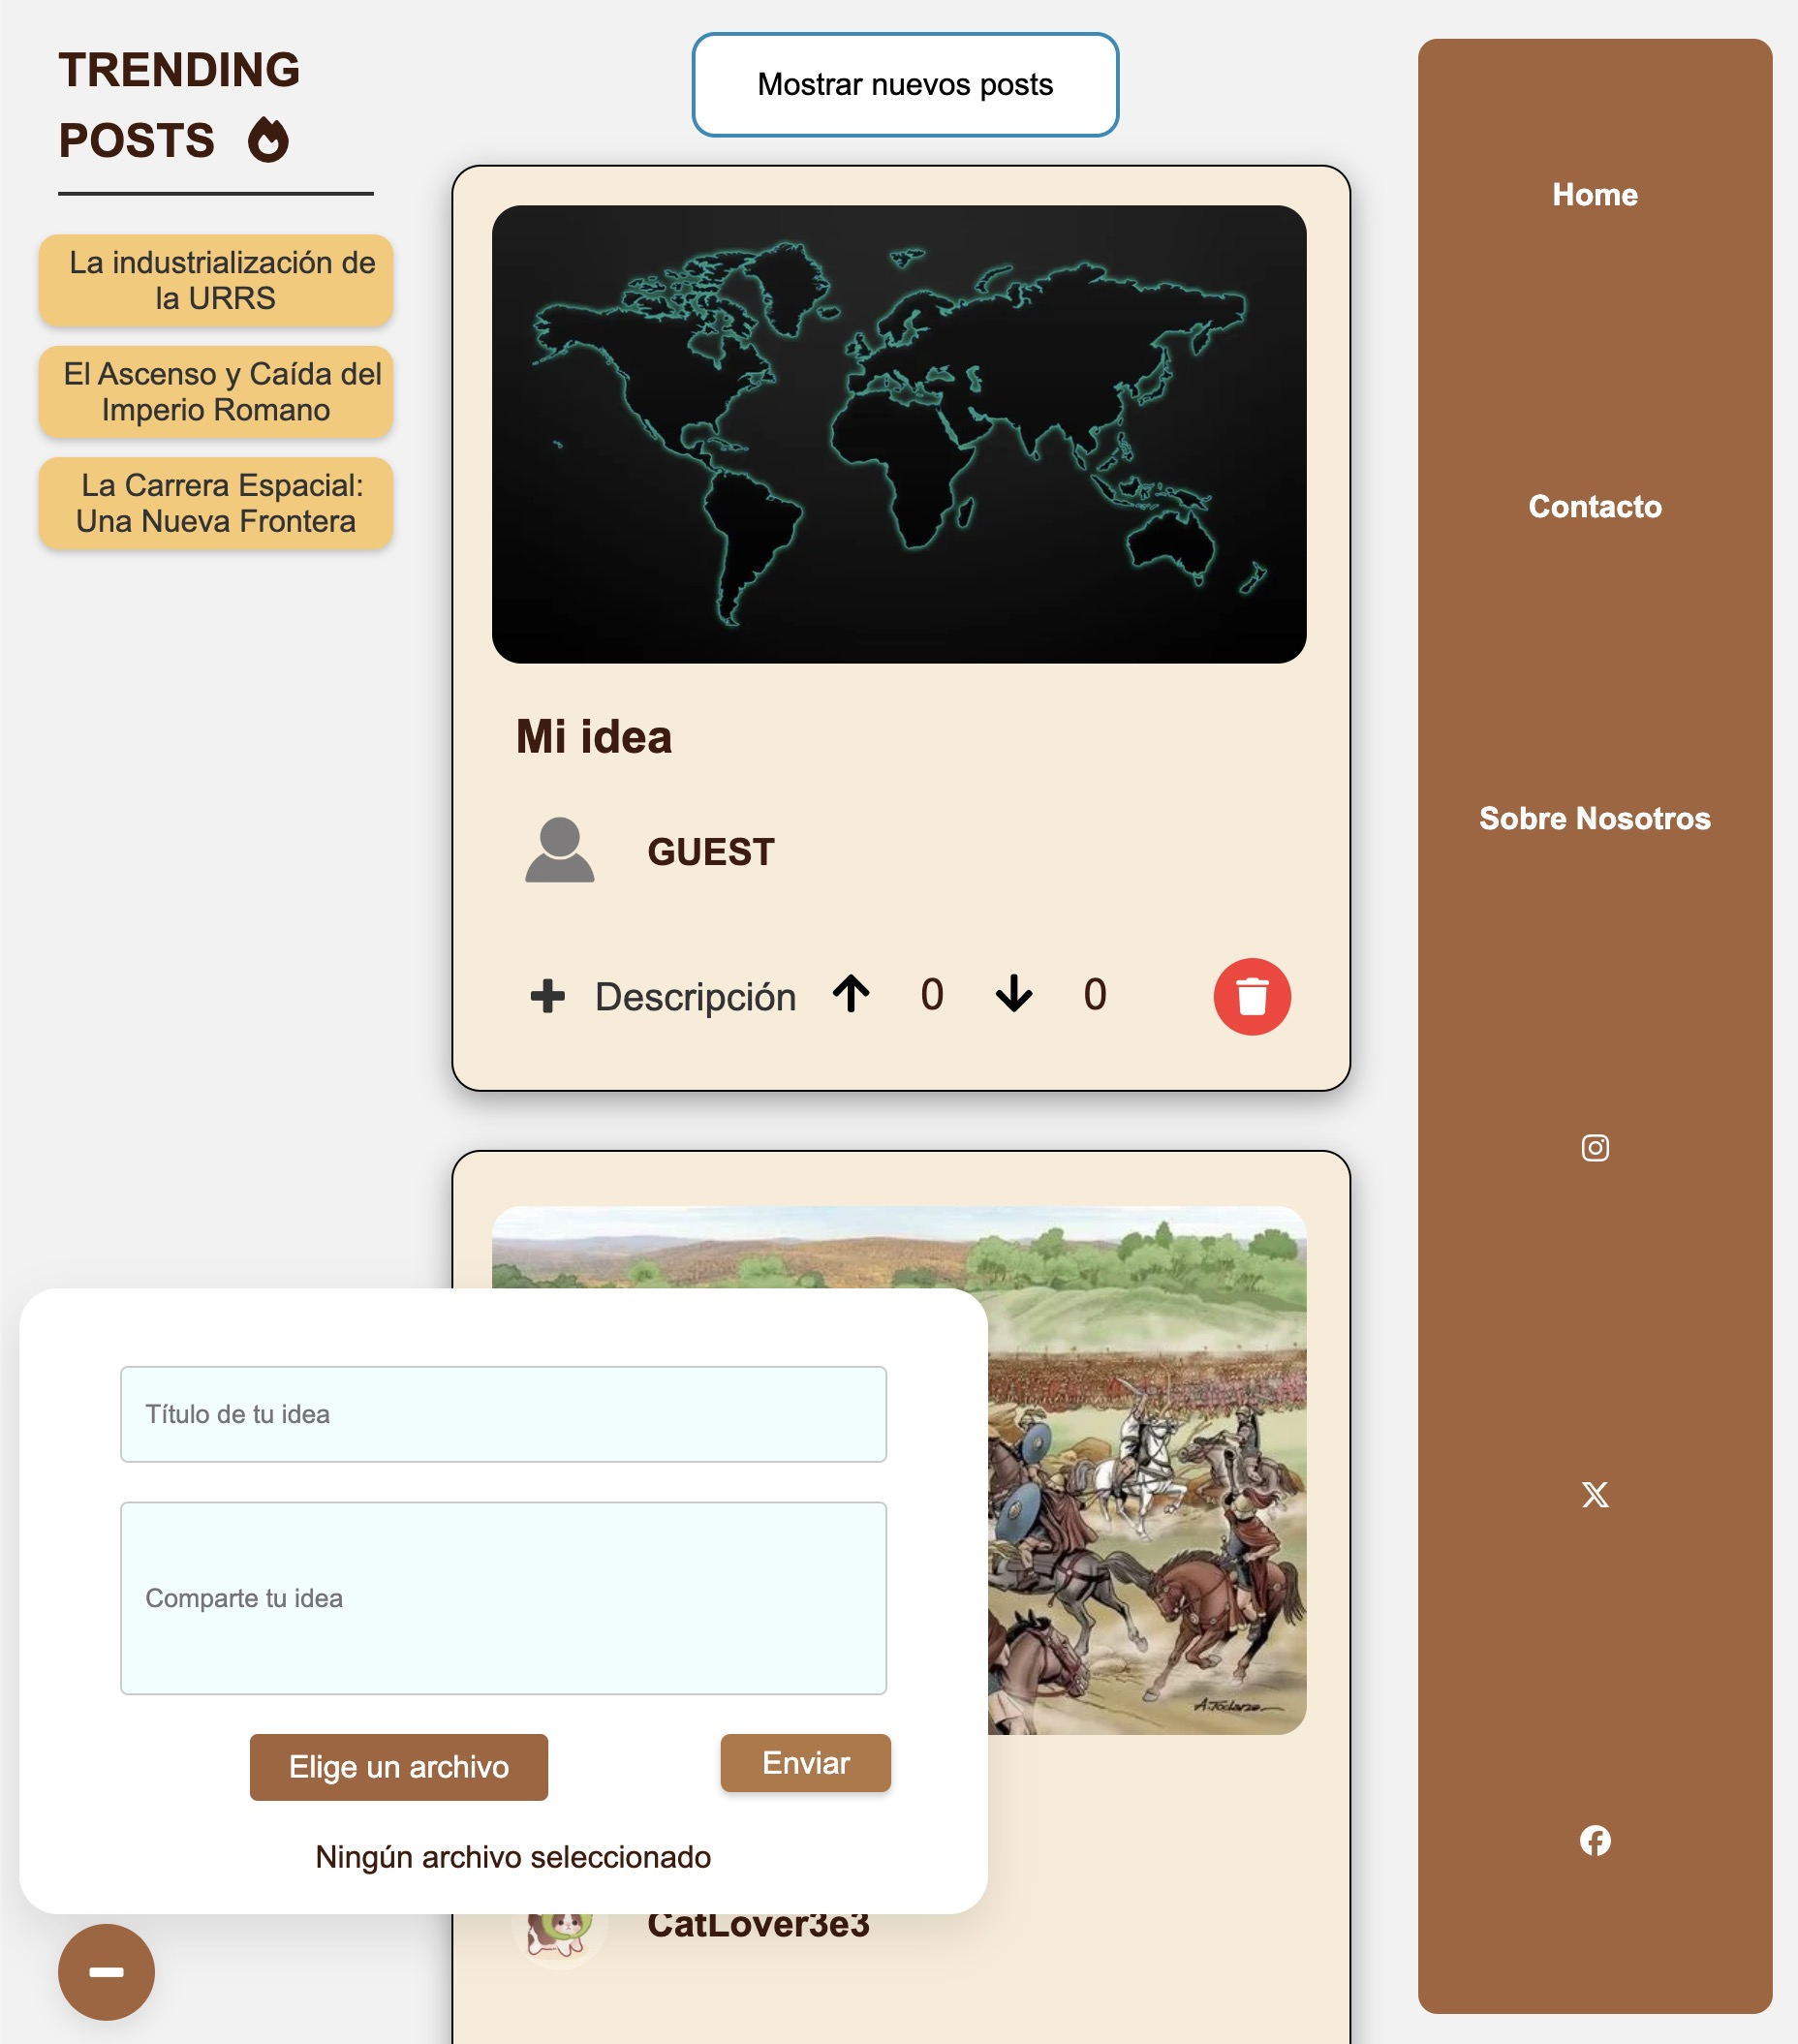
\includegraphics[width=\linewidth]{htmlFotos/foro.jpg}
        \caption{Interfaz de foro.html}
        \label{fig:foro_interface}
    \end{minipage}\hfill
    % Segunda imagen (derecha)
    \begin{minipage}{0.49\textwidth}
        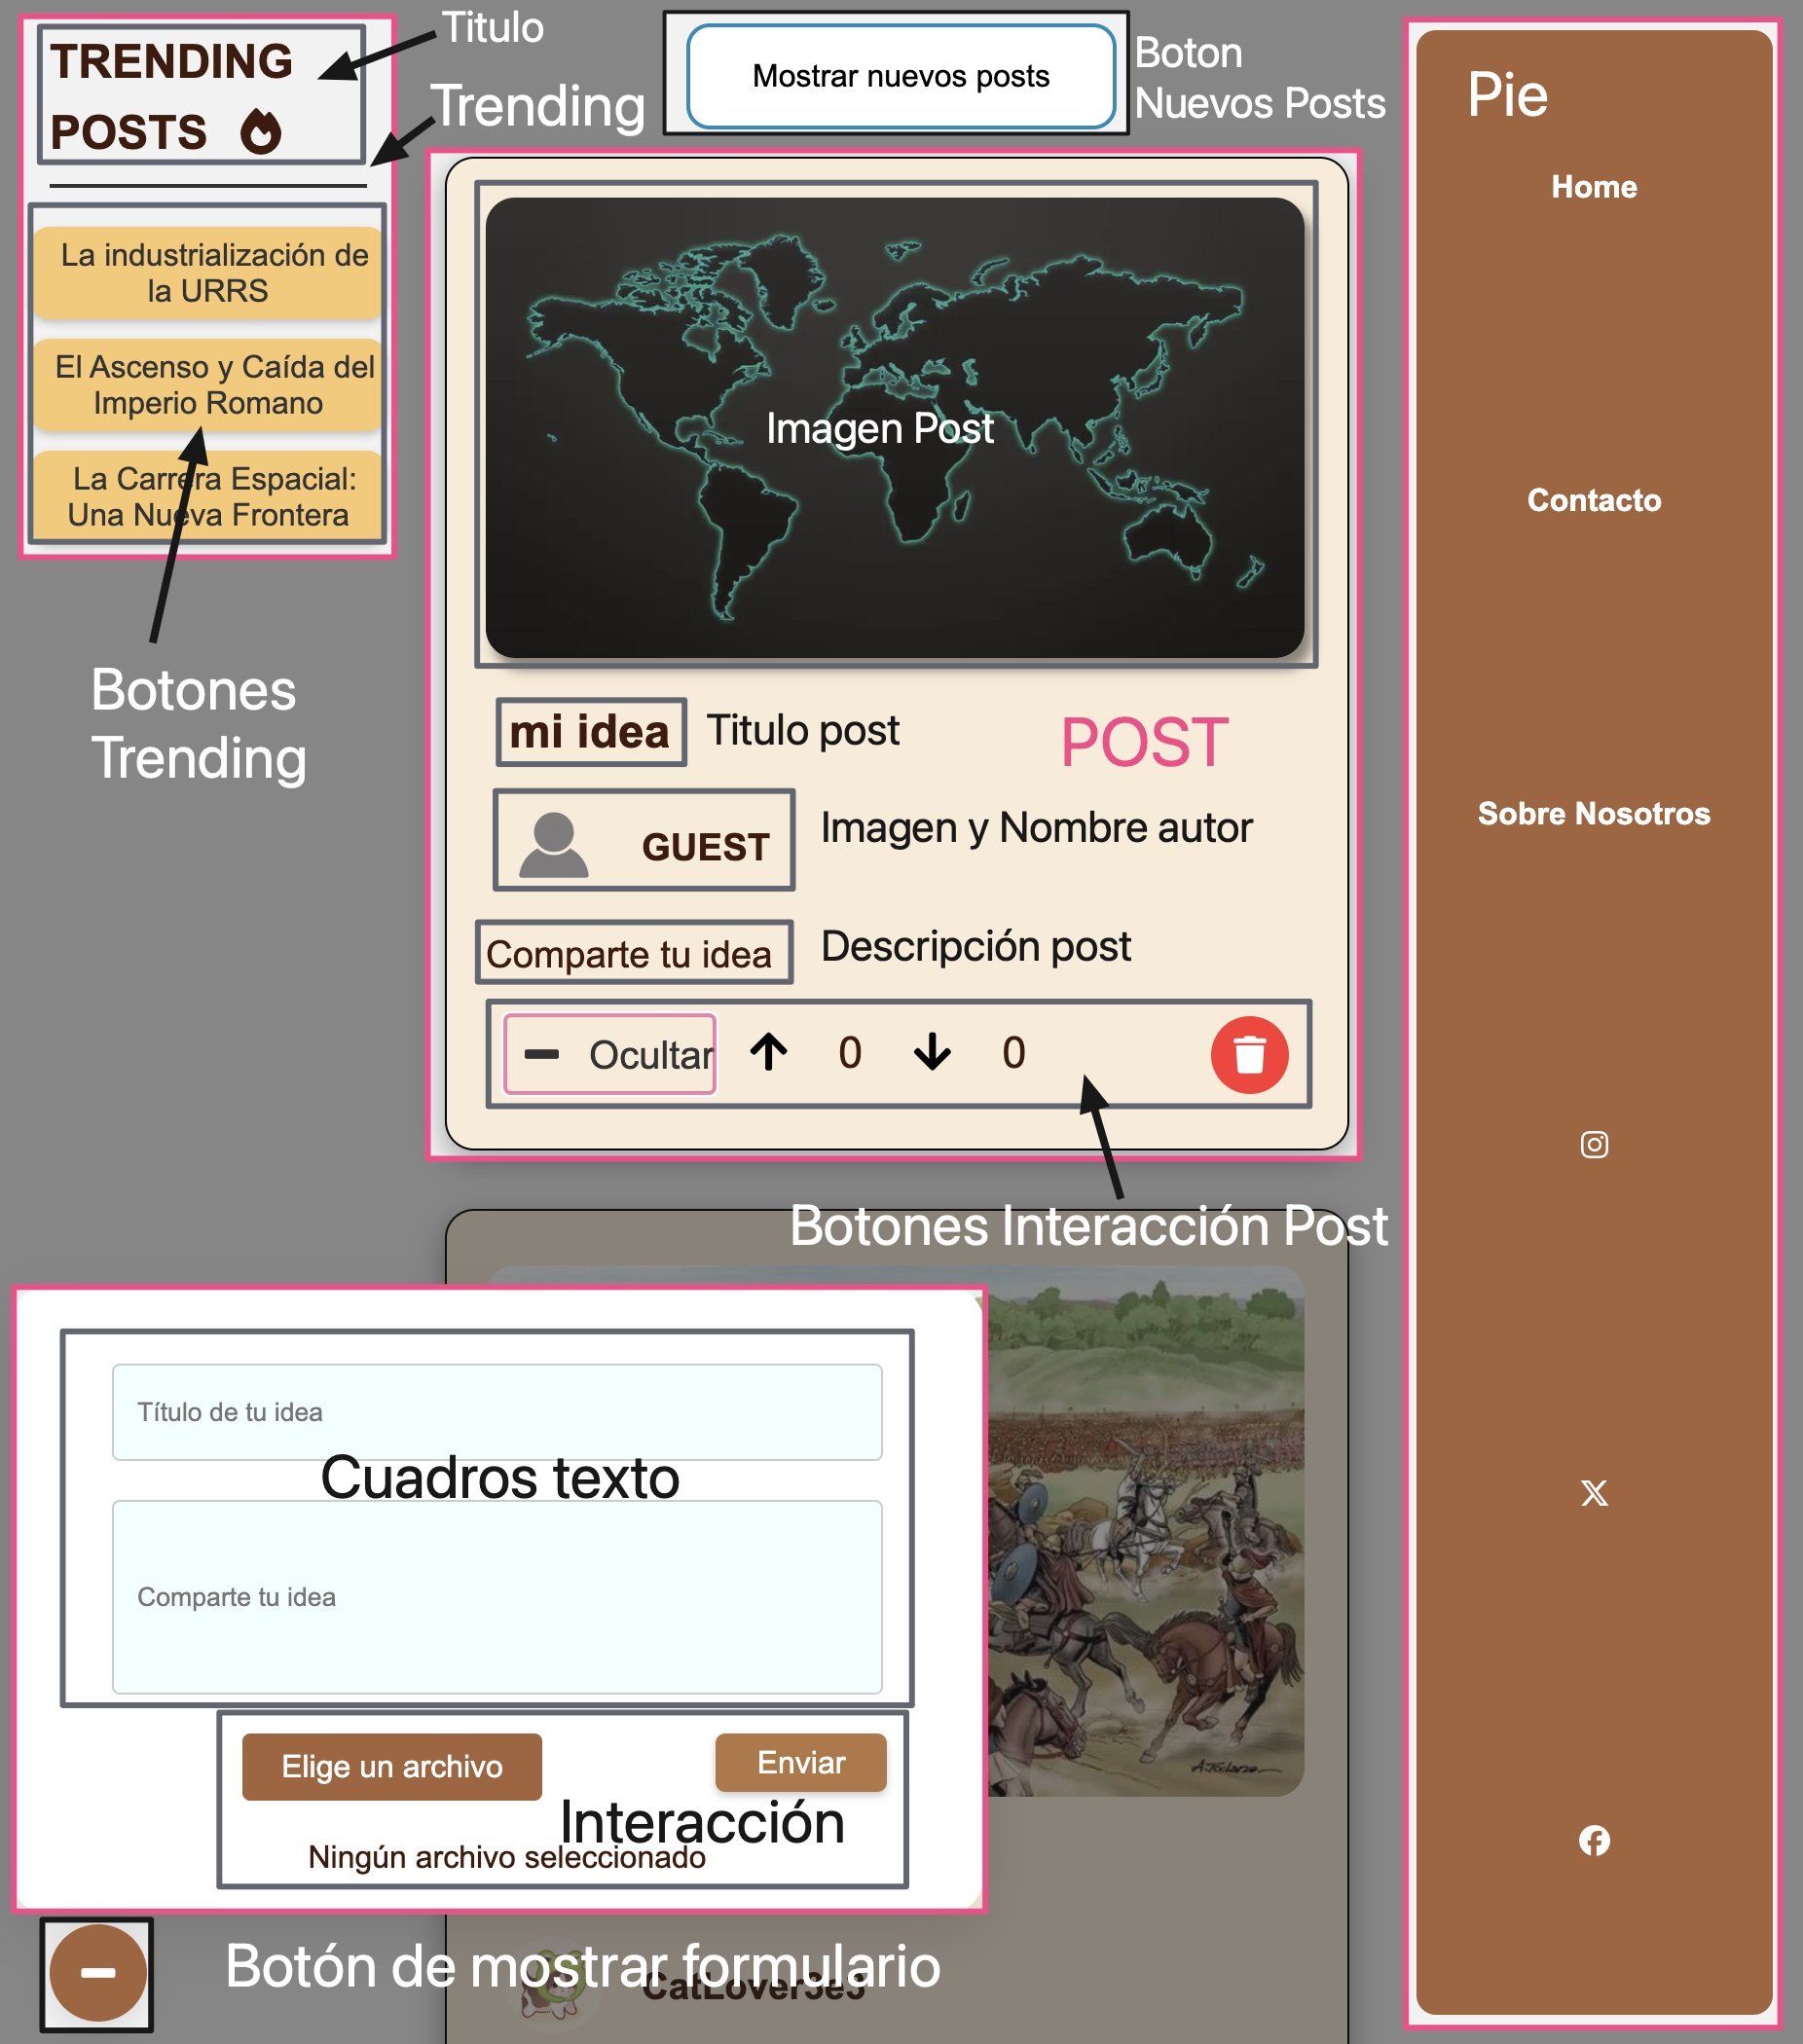
\includegraphics[width=\linewidth]{htmlFotos/prototipoForo.jpg}
        \caption{Prototipo de interfaz de foro.html}
        \label{fig:prototipo_foro}
    \end{minipage}
\end{figure}

% Espacio adicional para separar las figuras si es necesario
\vspace{10mm}

\begin{figure}[H]
    \centering
    % Tercera imagen (debajo, en una figura diferente)
    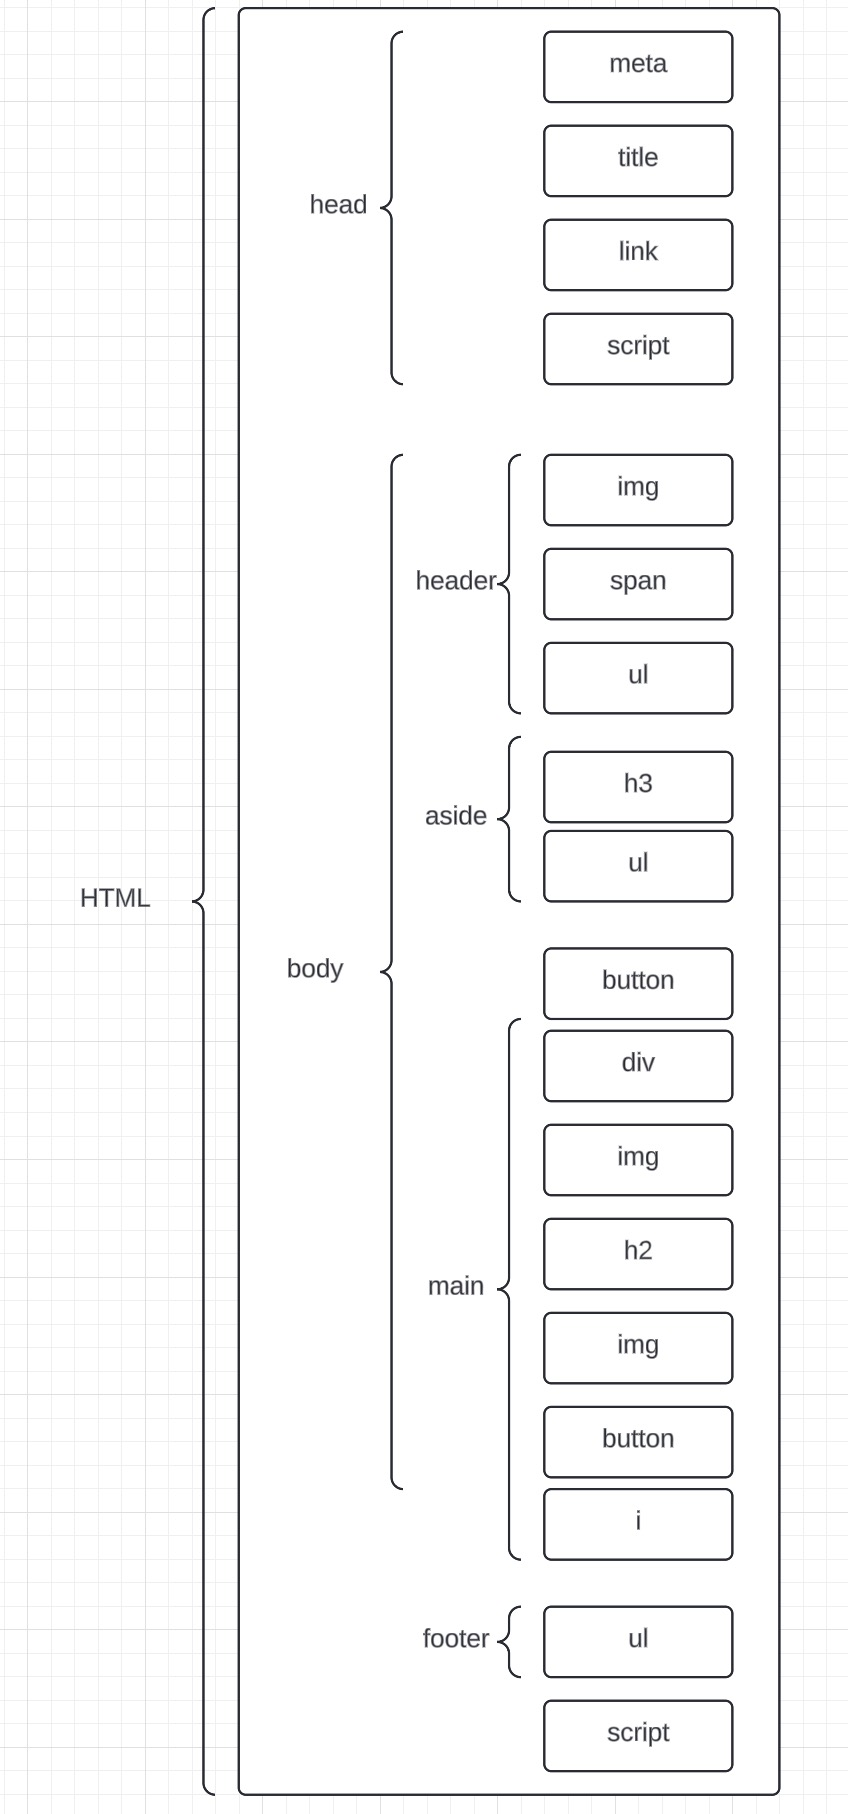
\includegraphics[width=\textwidth, height=0.8\textheight, keepaspectratio]{htmlFotos/MEforo.jpg}
    \caption{Mapa de etiquetas de foro.html}
    \label{fig:mapa_etiquetas_foro}
\end{figure}

\subsection{Estructura de ficheros actualizada}

\begin{figure}[H]
    \centering
    % Tercera imagen (debajo, en una figura diferente)
    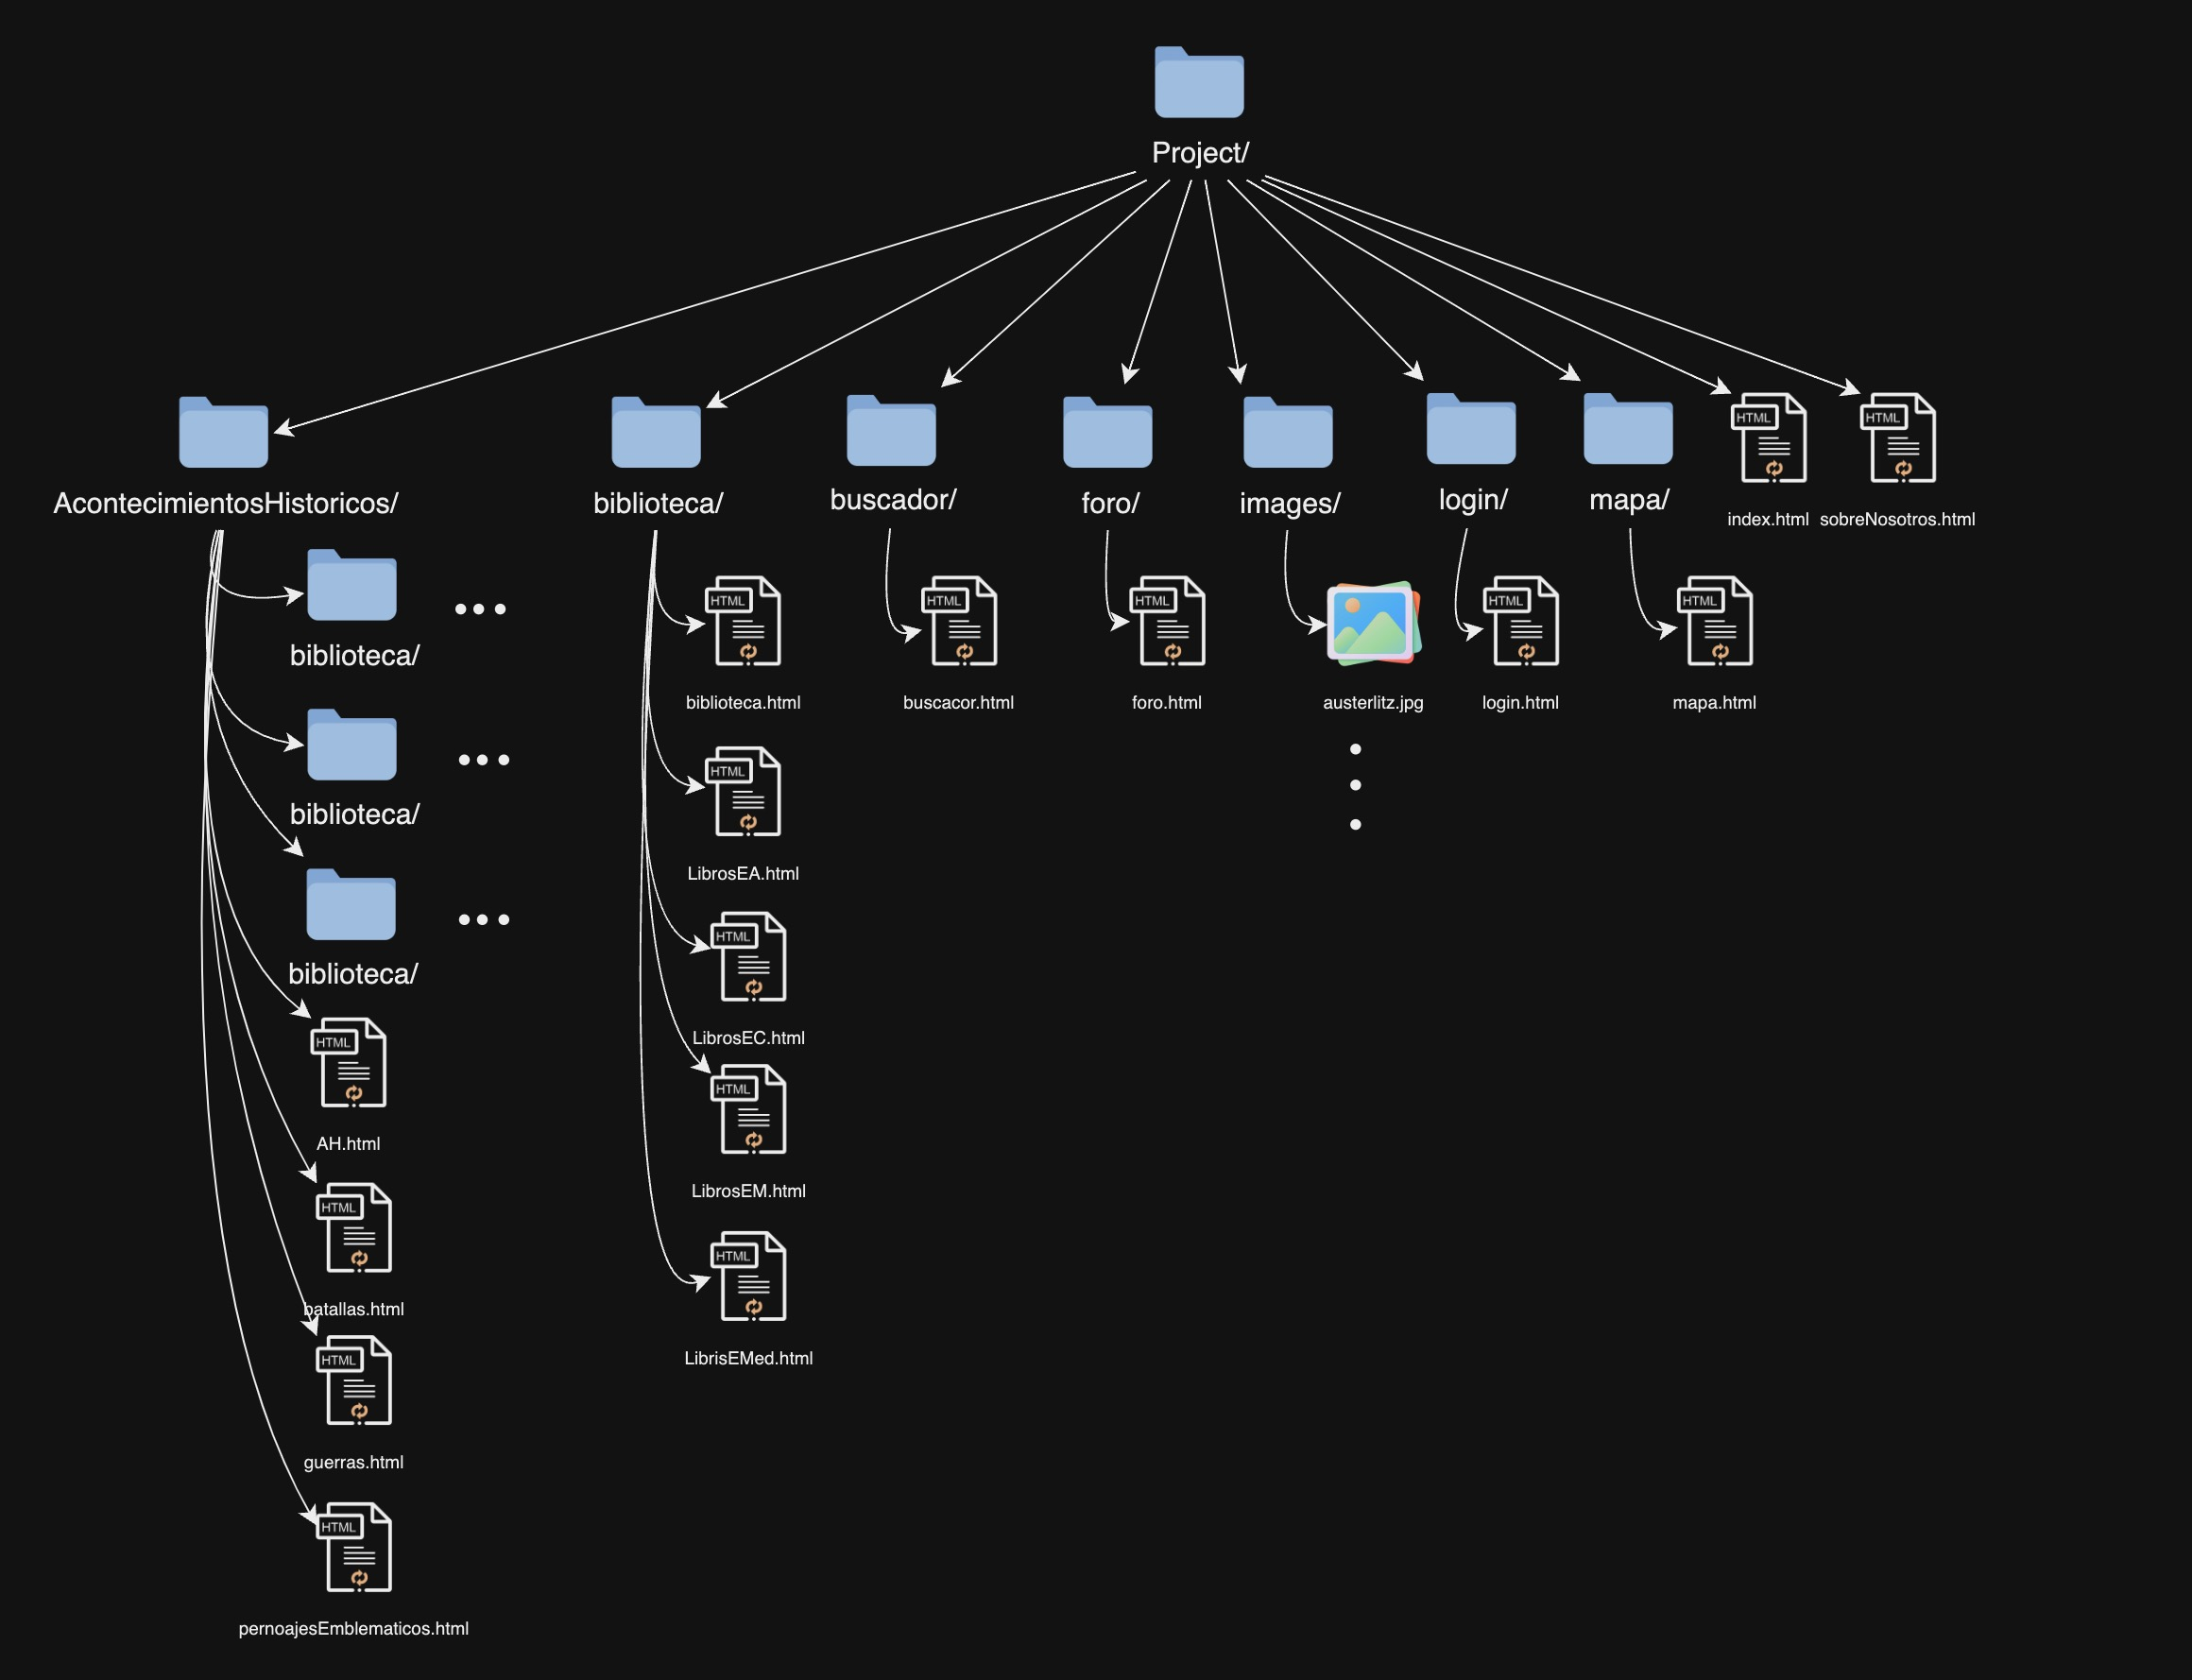
\includegraphics[width=\textwidth, height=0.8\textheight, keepaspectratio]{htmlFotos/estructuraFichero1.png}
    \caption{Estructura de ficheros actualizada}
    \label{fig:mapa_etiquetas_foro}
\end{figure}

\newpage

\section{CSS}

Durante esta fase del desarrollo, incluimos en nuestra página web hojas de estilo CSS para mejorar la presentación y el diseño de las páginas. Deberemos implementar 5 técnicas de diseño CSS responsivo:

\begin{itemize}
    \item \textbf{Flexible Grids}: aplicado en diversas páginas, como en biblioteca.html 
    \item \textbf{CSS Multicol}: En la página multicol.css aplicada en LibrosEM.html
    \item \textbf{Flex Container}:En la página flexcontainer.css aplicada en LibrosEC.html
    \item \textbf{CSS Grid}: En la página CSSgrid.css aplicada en LibrosEMed.html
    \item \textbf{Bootstrap}: En la página bootstrap.css y bootstrap.min.css (así como la inclusión de diversas librerías de Bootstrap) aplicada en LibrosEA.html, asi como en las páginas de inicio de acontencimientos históricos, batallas y personajes emblemáticos.
\end{itemize}

\subsection{Flexible Grids}

\begin{figure}[H]
    \centering
    % Primera imagen (izquierda)
    \begin{minipage}{0.49\textwidth}
        
\includegraphics[width=\linewidth]{cssFotos/flexibleGrids.jpg}
        \caption{Interfaz de biblioteca.html}
        \label{fig:foro_interface}
    \end{minipage}\hfill
    % Segunda imagen (derecha)
    \begin{minipage}{0.49\textwidth}
        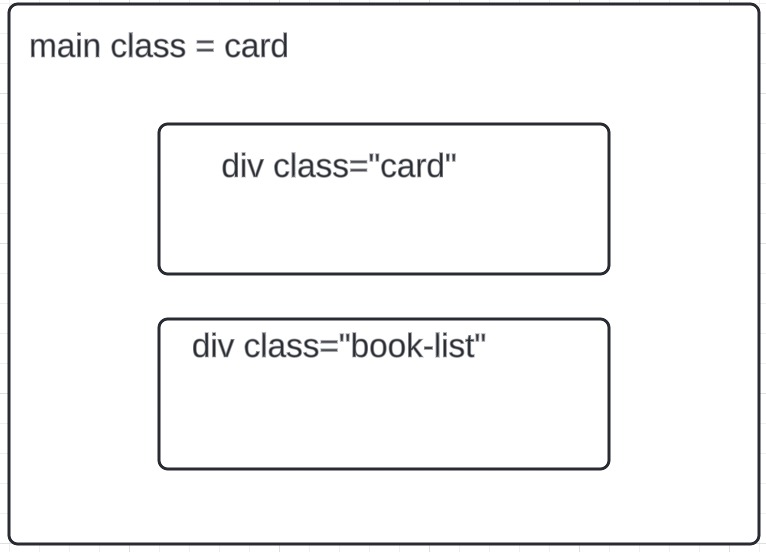
\includegraphics[width=\linewidth]{cssFotos/flexibleGridsEsquema.jpg}
        \caption{Prototipo de interfaz de biblioteca.html}
        \label{fig:prototipo_foro}
    \end{minipage}
\end{figure}

\subsection{CSS Multicol}

\begin{figure}[H]
    \centering
    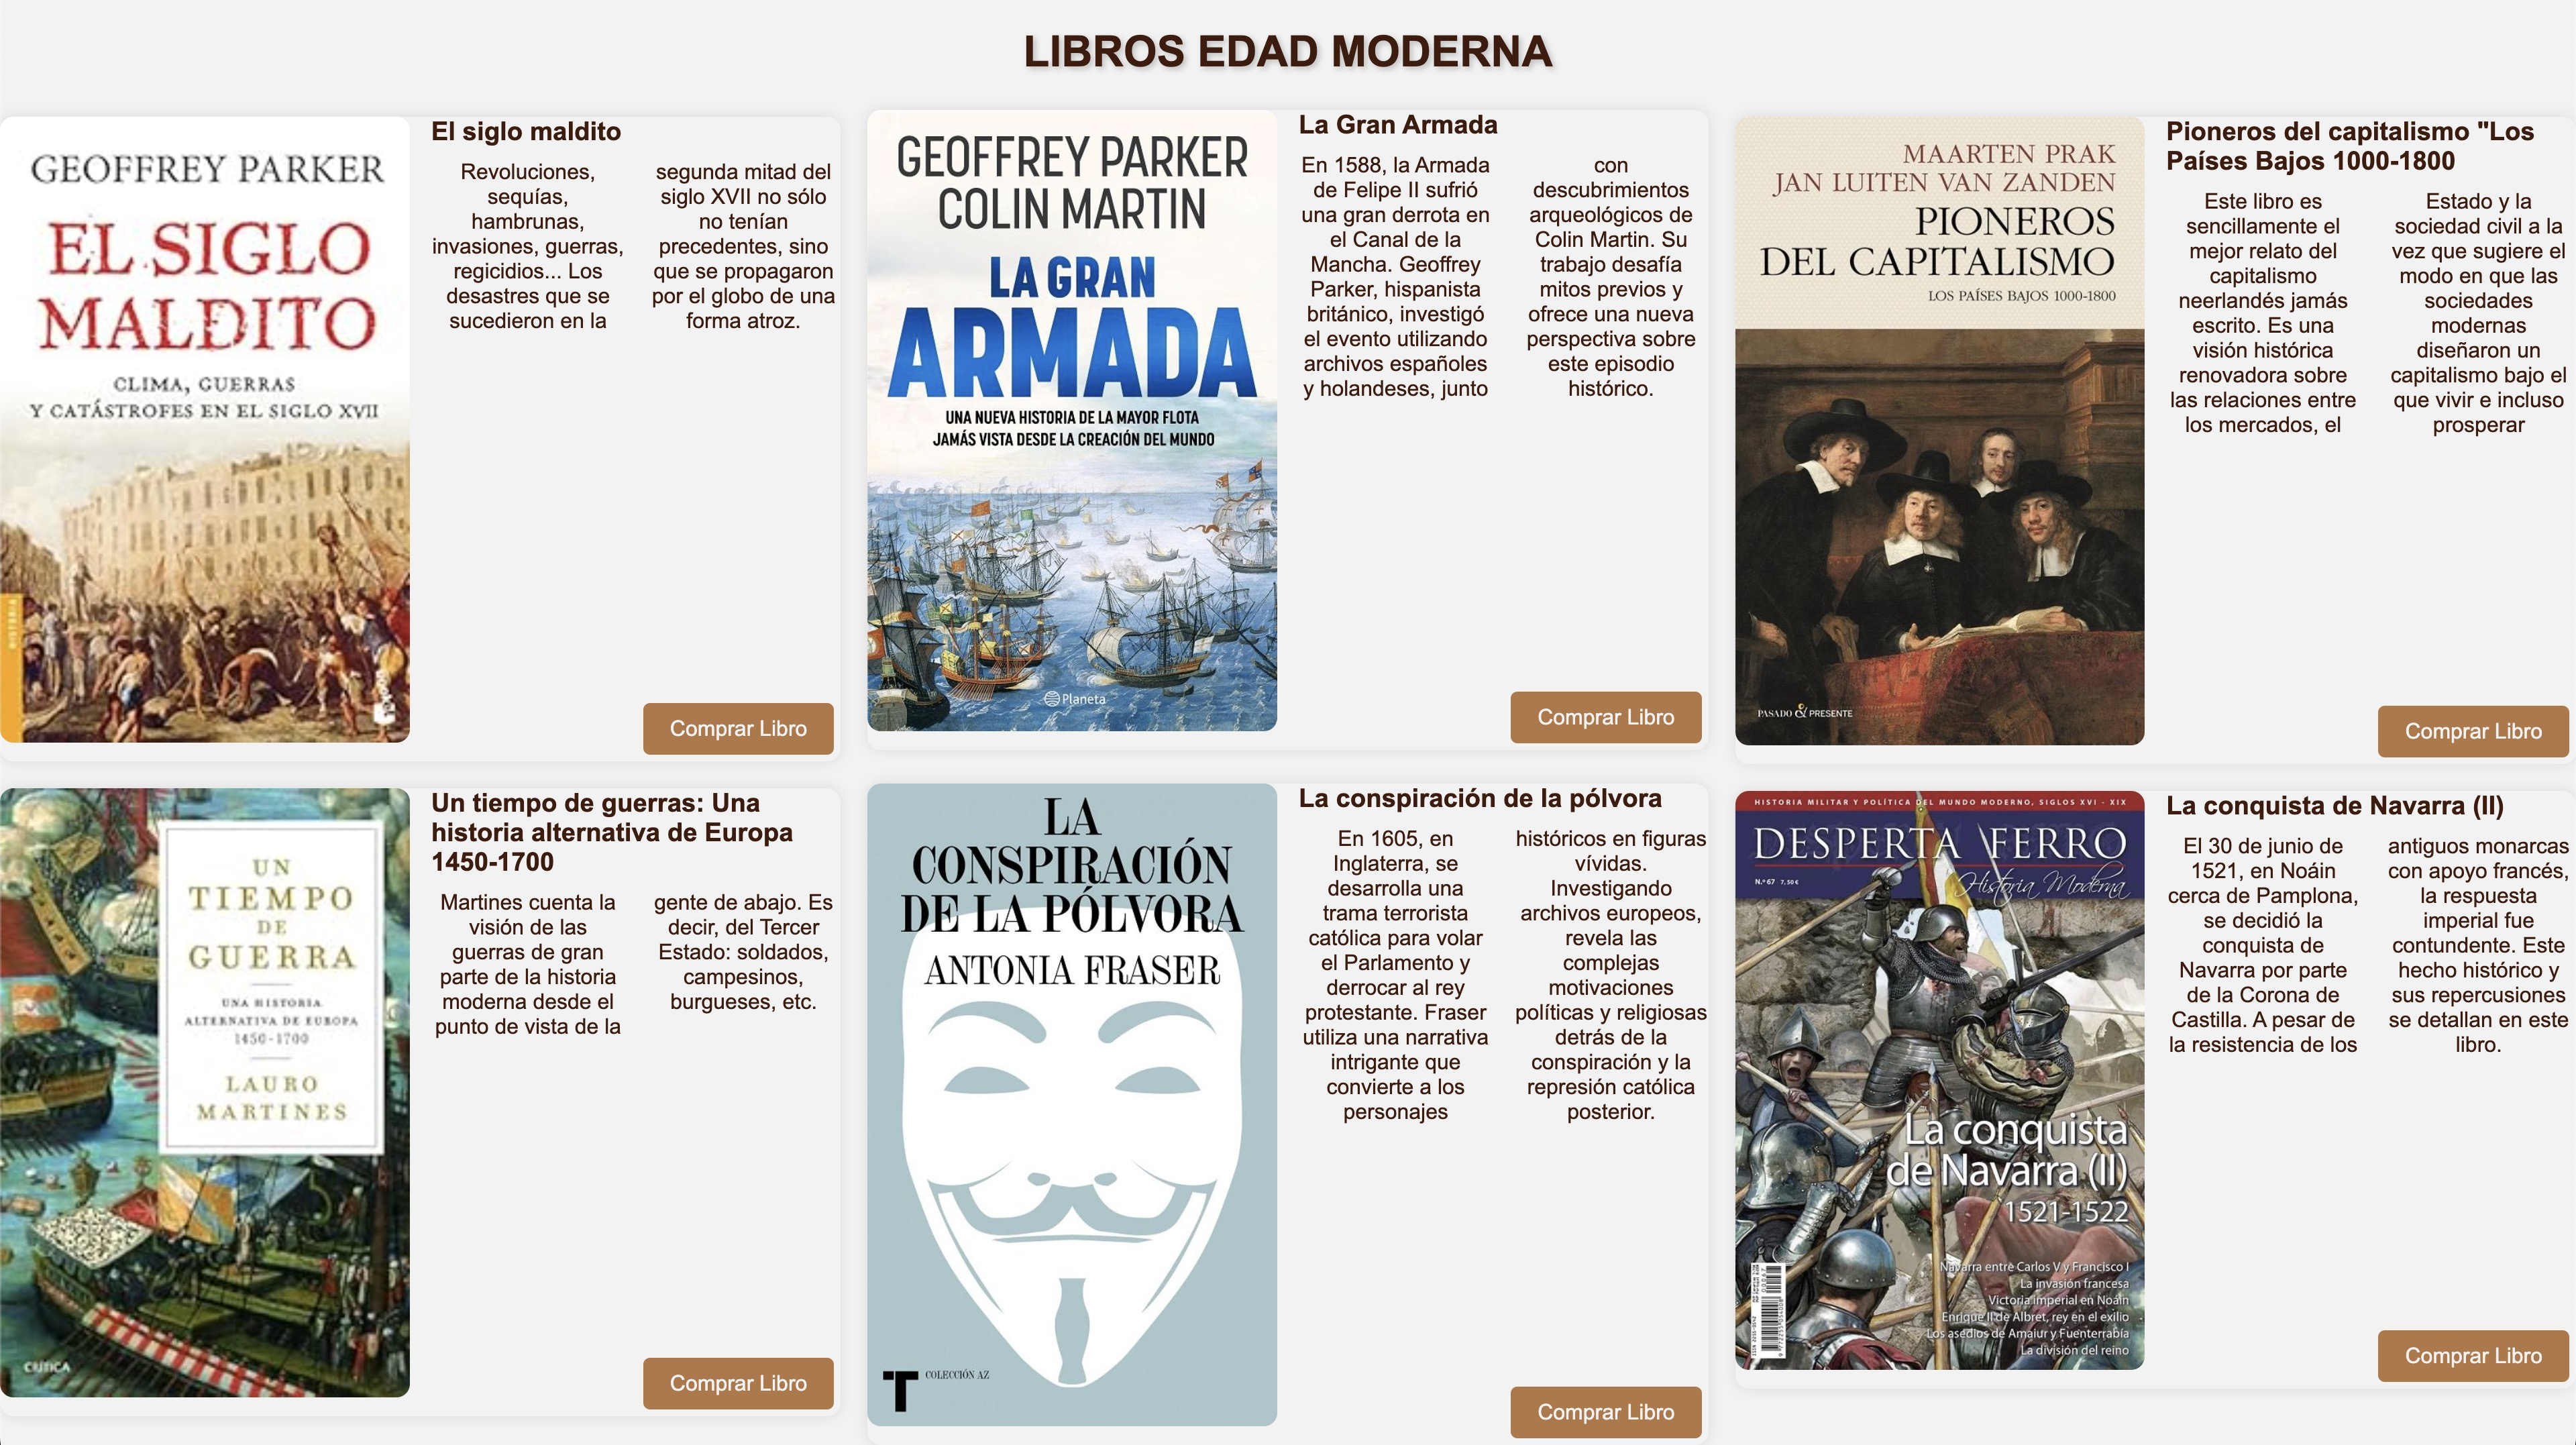
\includegraphics[width=1\textwidth]{cssFotos/multicol.jpg}
    \caption{Interfaz de LibrosEM.html}
    \label{fig:foro_interface}
\end{figure}

\begin{figure}[H]
    \centering
    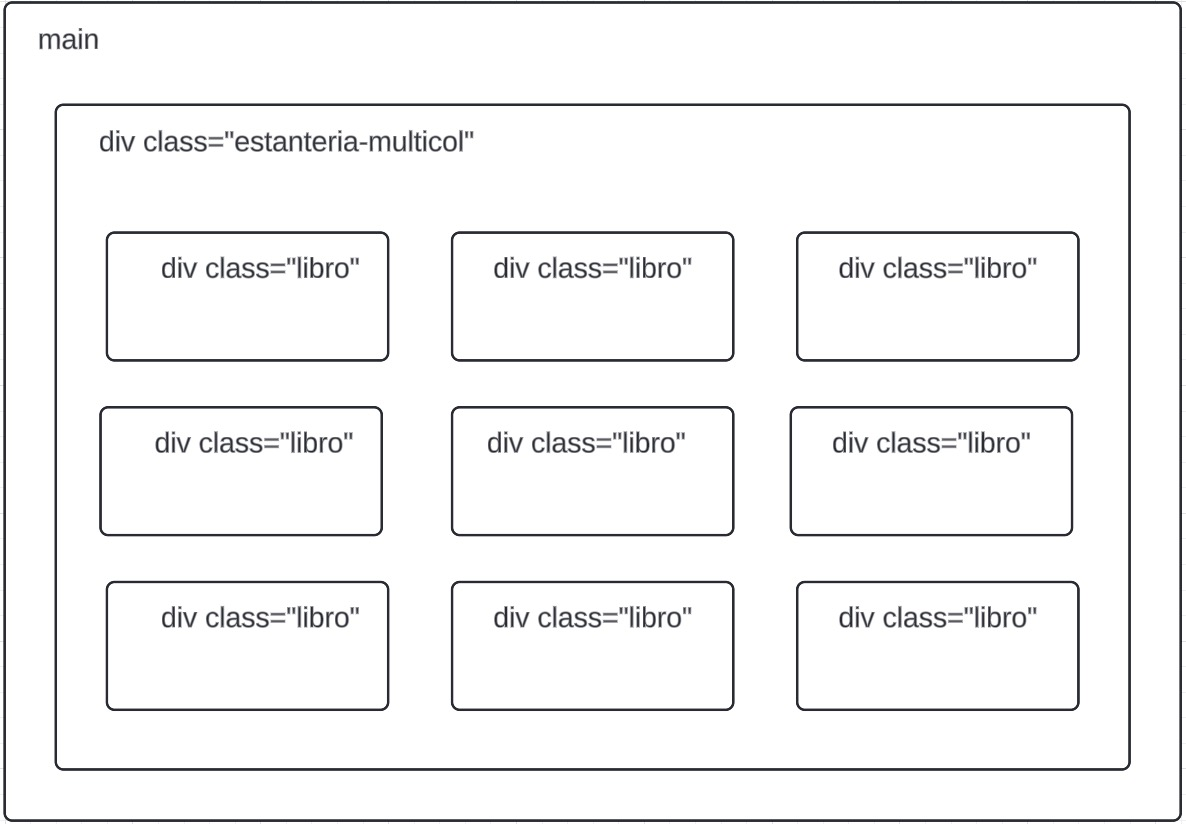
\includegraphics[width=0.6\textwidth]{cssFotos/multicolEsquema.jpg}
    \caption{Prototipo de interfaz de LibrosEM.html}
    \label{fig:prototipo_foro}
\end{figure}


\newpage

\subsection{Flex Container}

\begin{figure}[H]
    \centering
    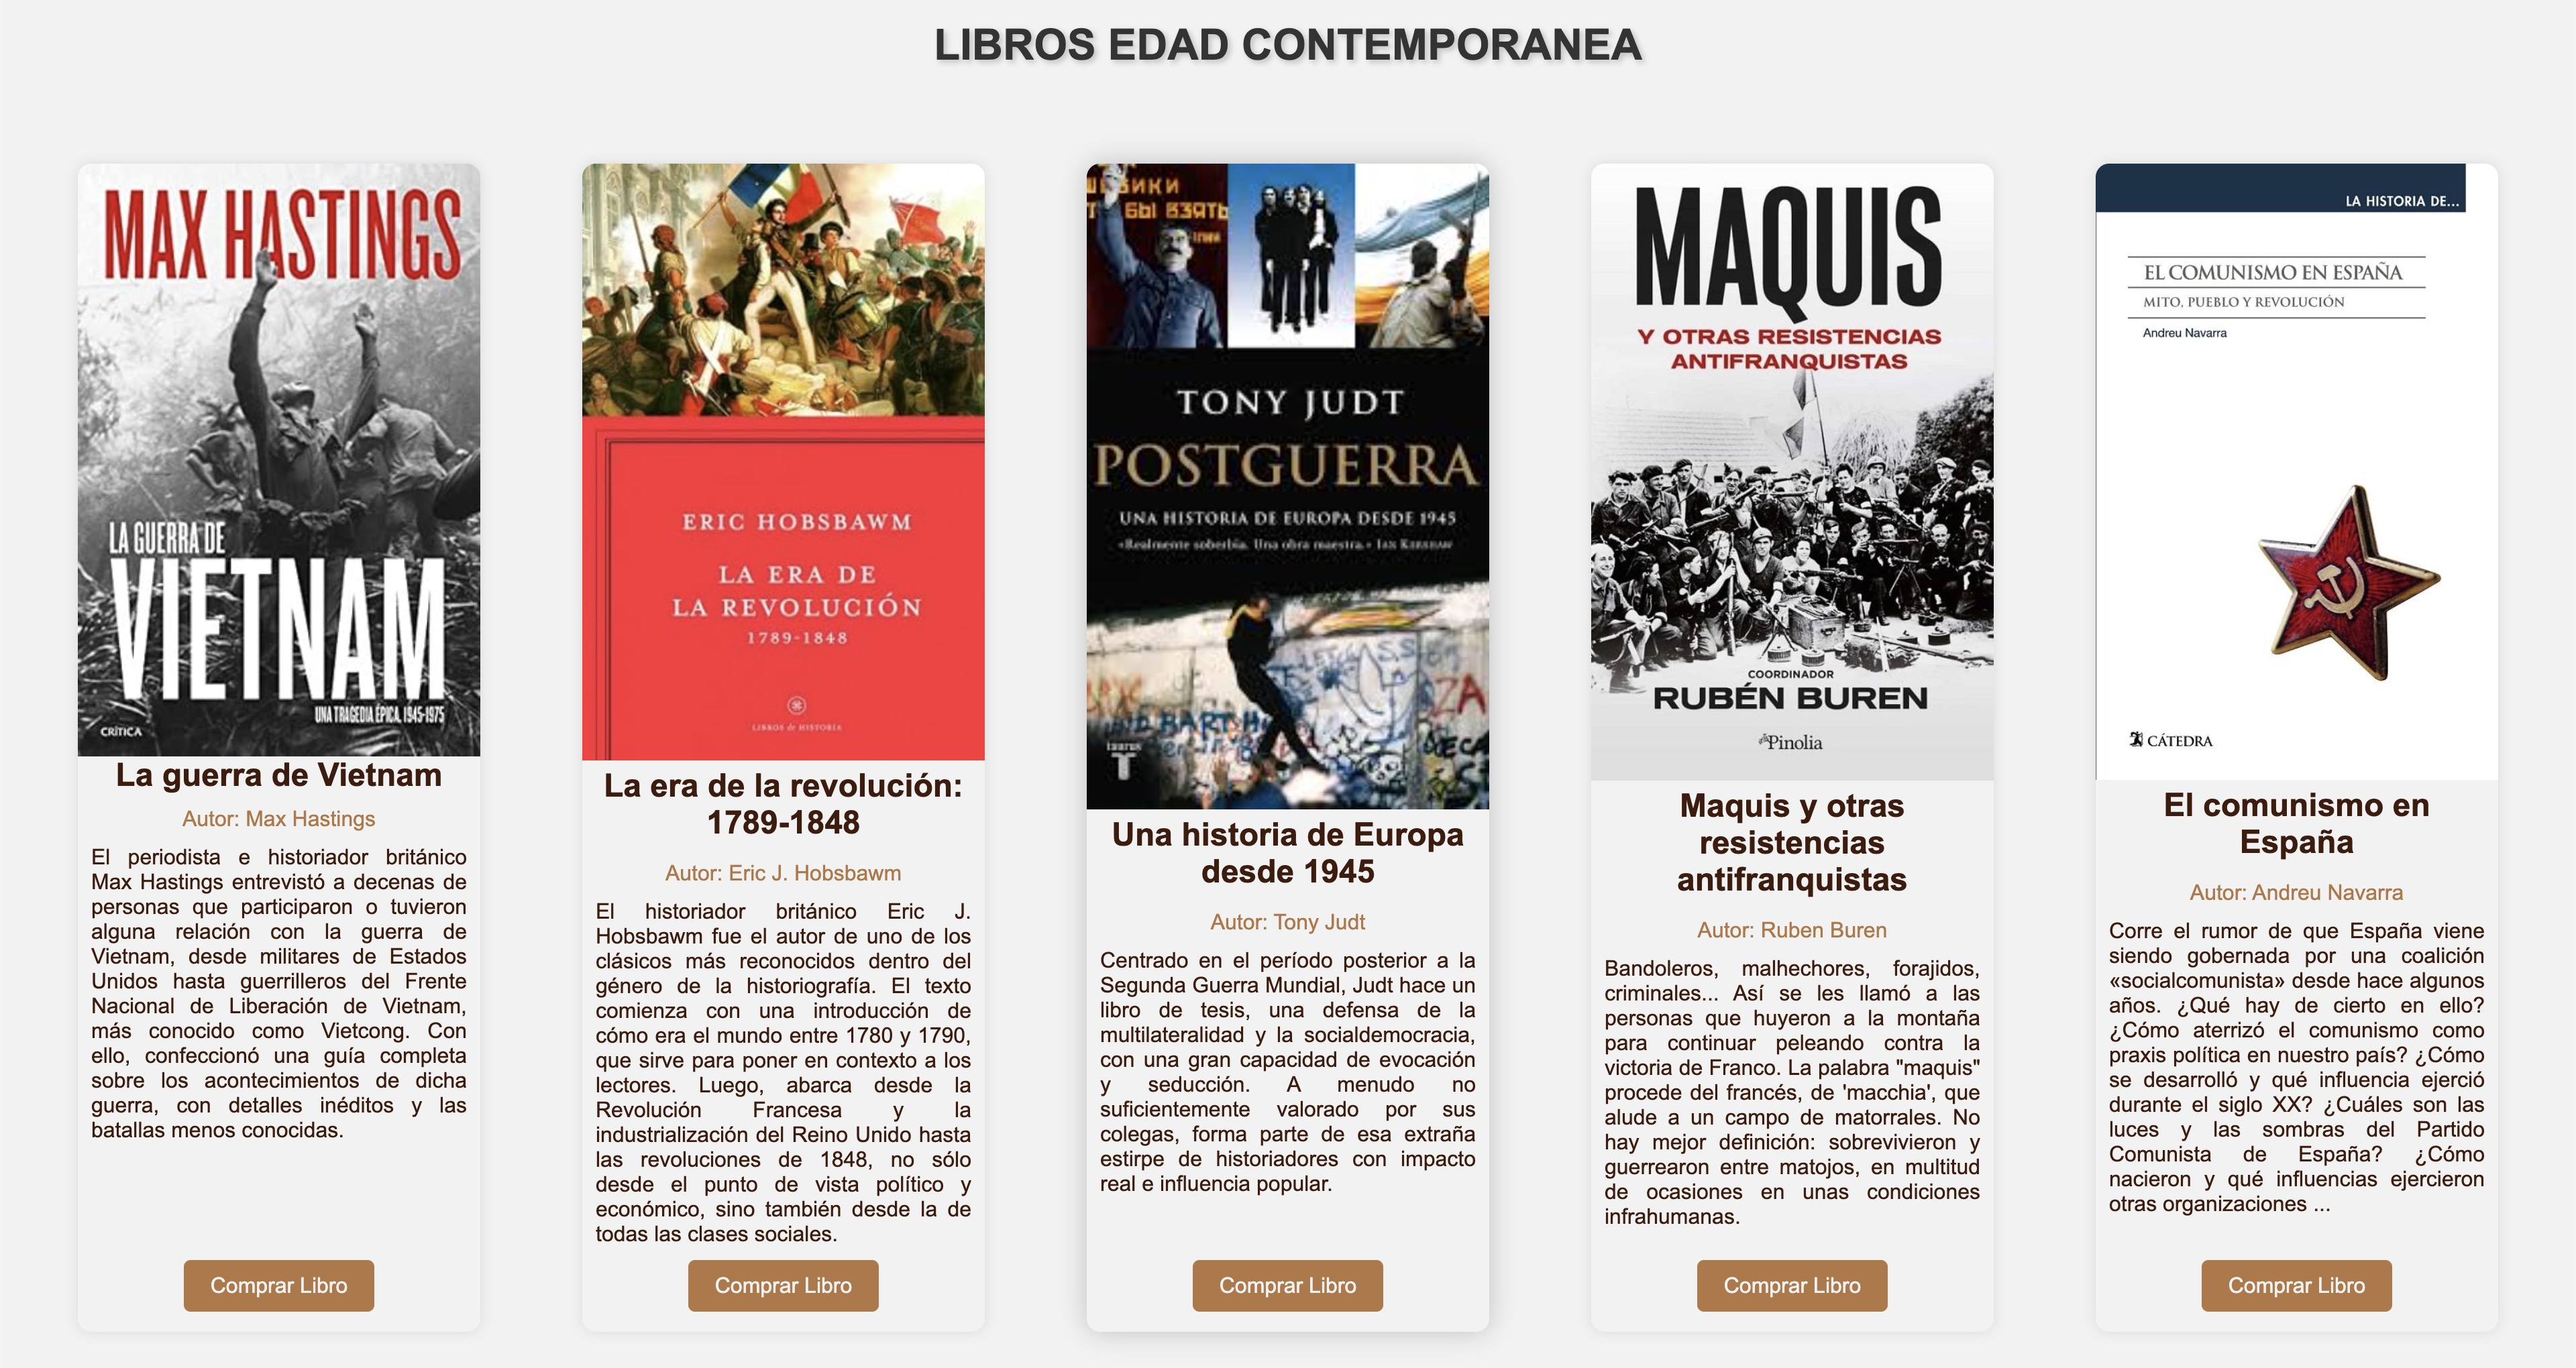
\includegraphics[width=1\textwidth]{cssFotos/flexContainer.jpg}
    \caption{Interfaz de LibrosEC.html}
    \label{fig:foro_interface}
\end{figure}

\begin{figure}[H]
    \centering
    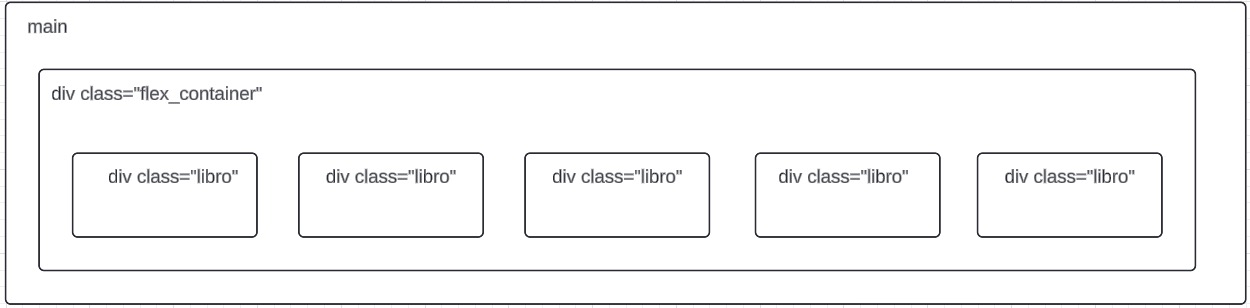
\includegraphics[width=1\textwidth]{cssFotos/flexContainerEsquema.jpg}
    \caption{Prototipo de interfaz de LibrosEC.html}
    \label{fig:prototipo_foro}
\end{figure}

\subsection{CSS Grid}

\begin{figure}[H]
    \centering
    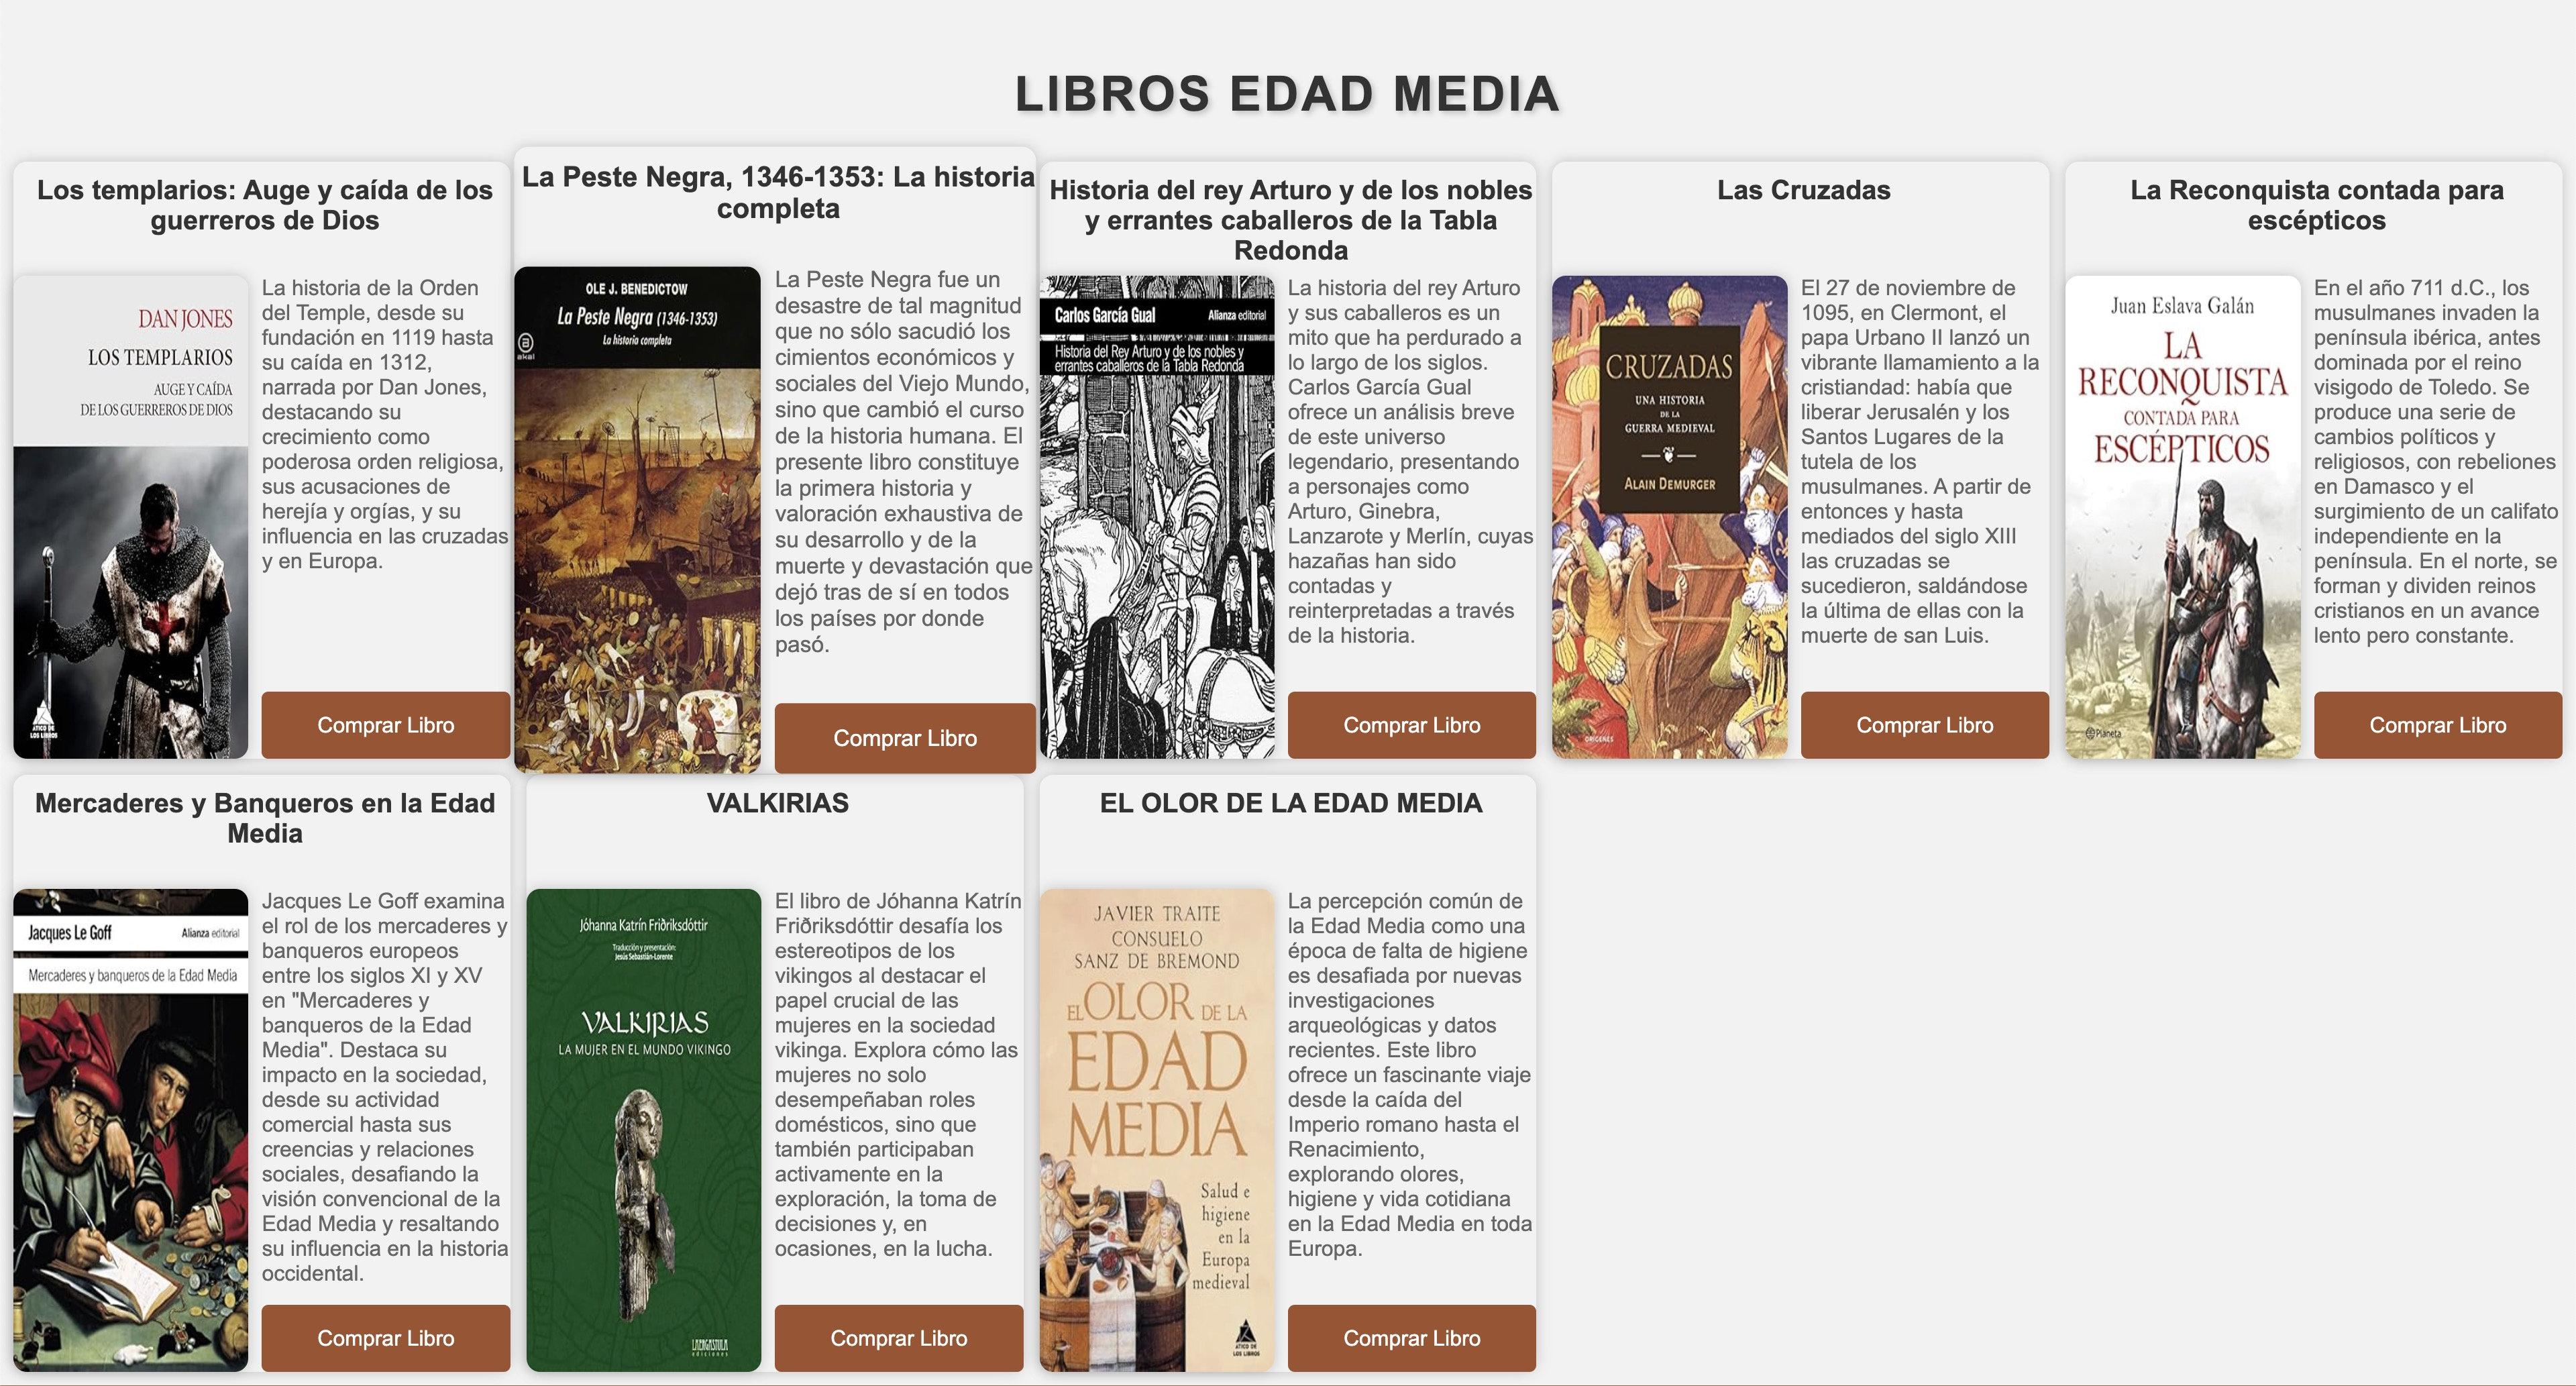
\includegraphics[width=1\textwidth]{cssFotos/cssgrid.jpg}
    \caption{Interfaz de LibrosEMed.html}
    \label{fig:foro_interface}
\end{figure}

\begin{figure}[H]
    \centering
    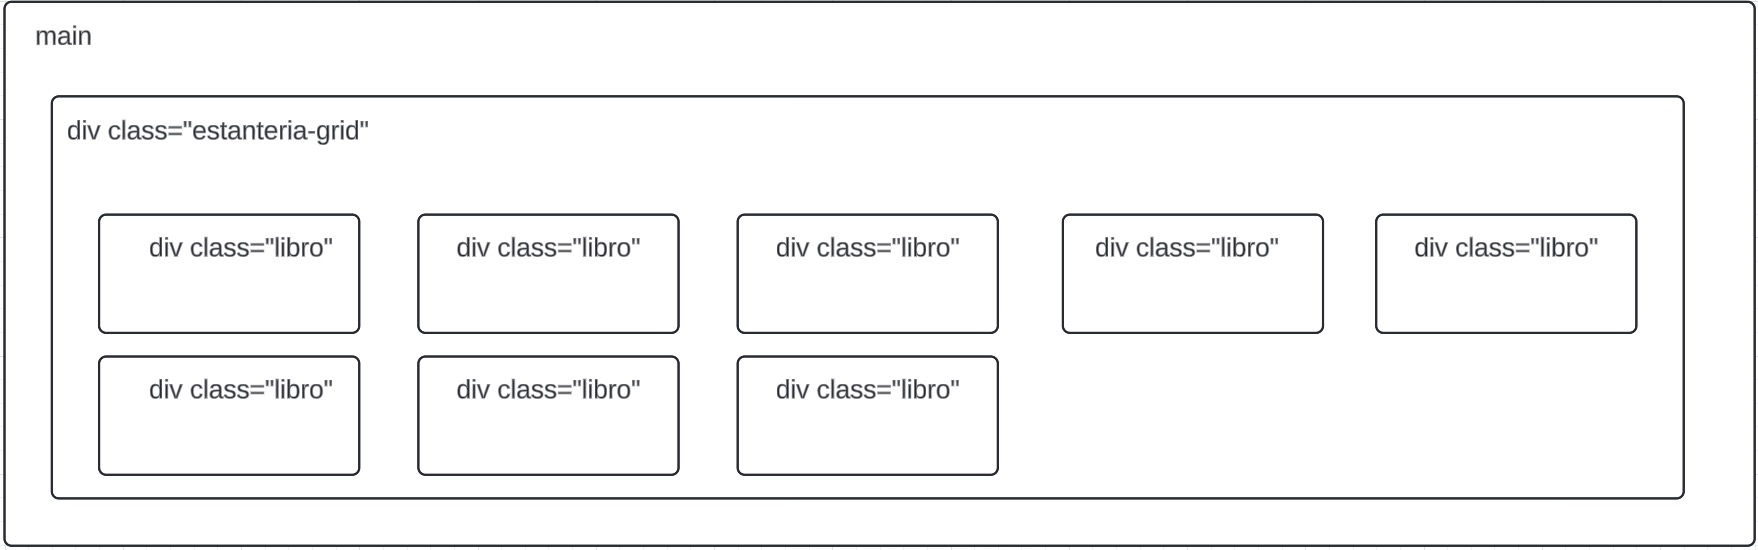
\includegraphics[width=1\textwidth]{cssFotos/cssgridEsquema.jpg}
    \caption{Prototipo de interfaz de LibrosEMed.html}
    \label{fig:prototipo_foro}
\end{figure}

\subsection{Bootstrap}

\begin{figure}[H]
    \centering
    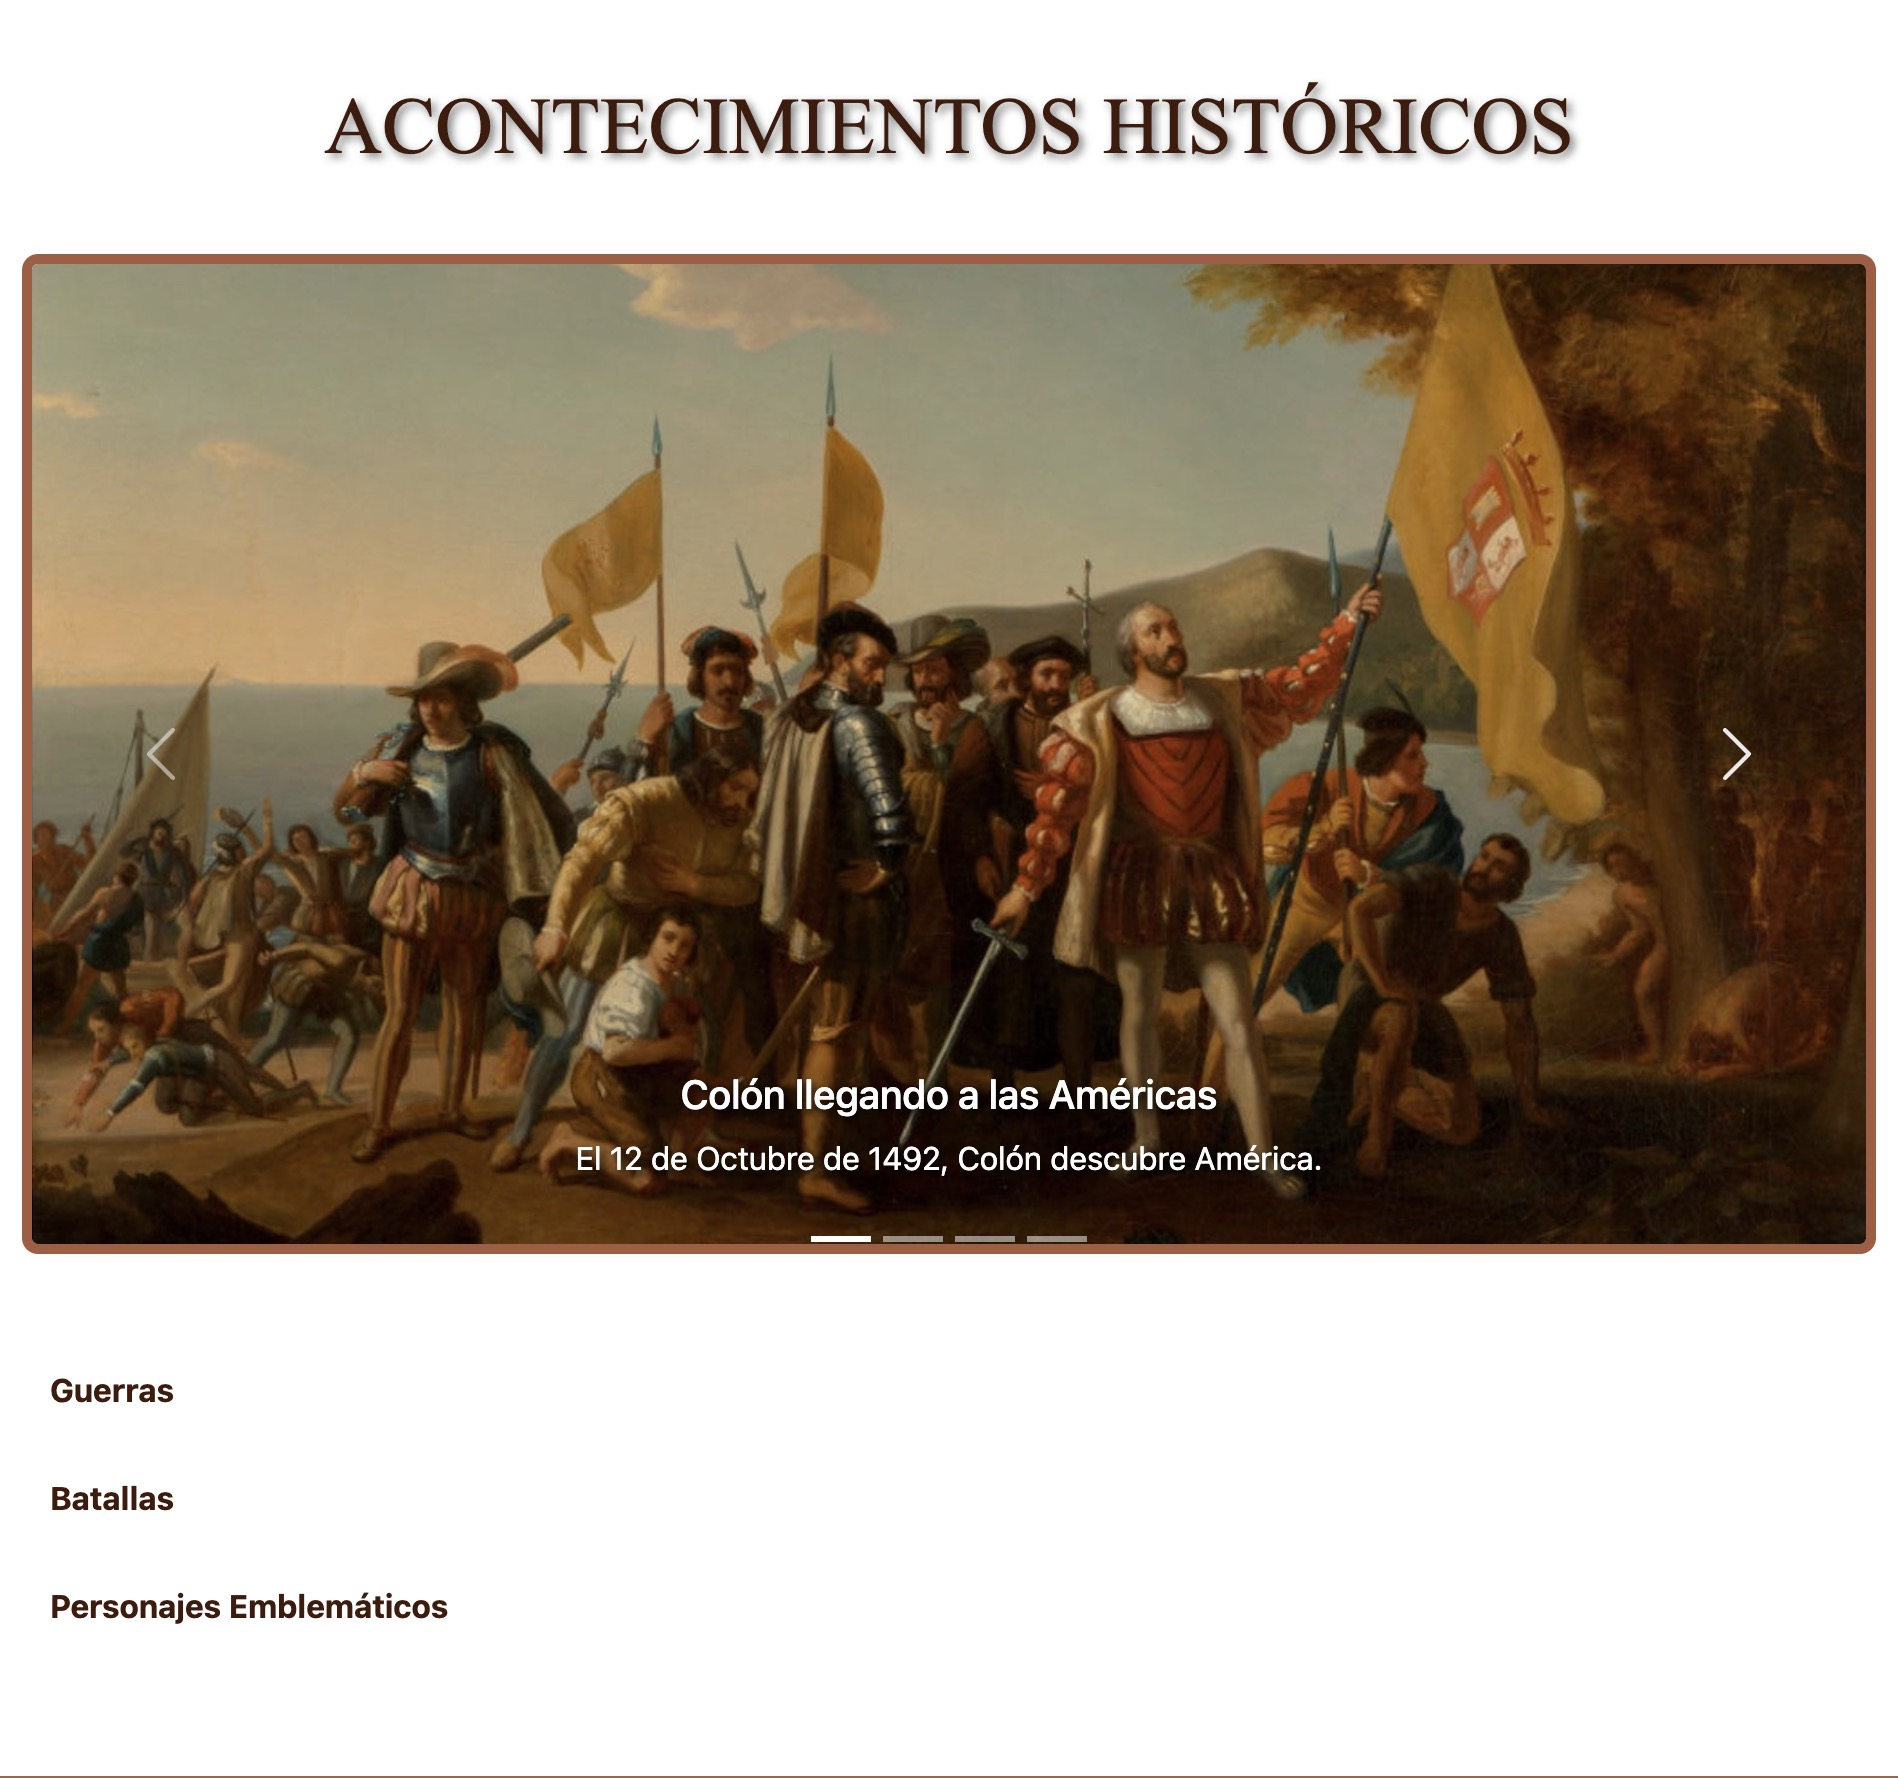
\includegraphics[width=0.7\textwidth]{cssFotos/bootstrap.jpg}
    \caption{Interfaz de AH.html}
    \label{fig:foro_interface}
\end{figure}

\begin{figure}[H]
    \centering
    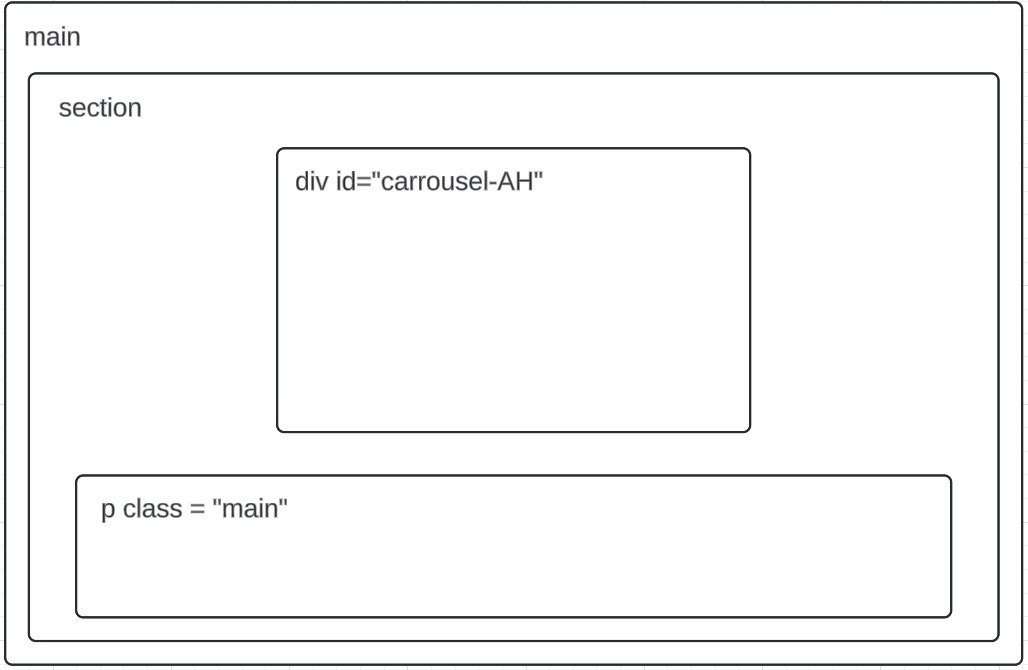
\includegraphics[width=0.7\textwidth]{cssFotos/bootstrapEsquema.jpg}
    \caption{Prototipo de interfaz de AH.html}
    \label{fig:prototipo_foro}
\end{figure}

También podremos ver como se ha aplicado esta librería en la página de LibrosEA.html.

\begin{figure}[H]
    \centering
    \includegraphics[width=0.7\textwidth]{cssFotos/LibrosEA.jpg}
    \caption{Interfaz de LibrosEA.html}
    \label{fig:foro_interface}
\end{figure}

\begin{figure}[H]
    \centering
    \includegraphics[width=0.7\textwidth]{cssFotos/LibrosEAEsquema.jpg}
    \caption{Prototipo de interfaz de LibrosEA.html}
    \label{fig:prototipo_foro}
\end{figure}

\newpage

\section{JavaScript}

En esta sección se presentan las funcionalidades de JavaScript implementadas en nuestra página web. Estas funciones permiten una interacción dinámica y enriquecedora con el contenido, mejorando la experiencia del usuario y facilitando la navegación a través de las distintas secciones del sitio.

\subsection{Funcionalidades}

En primer lugar mostraremos las funcionalidades de la aplicación, con sus correspondientes efectos en ella mediante capturas de pantalla.

\subsubsection{Header}

En primer lugar, cabe destacar el header, que se encuentra en todas las páginas de la web. En el header incorporamos una funcionalidad tal que, cuando la página web pasa uno de los puntos de ruptura (768 px), el menú de navegación se convierte en un menú desplegable, que se puede abrir y cerrar pulsando el botón de menú.

\begin{figure}[H]
    \centering
    \includegraphics[width=1\textwidth]{jsFotos/headerJS.jpg}
    \caption{Menú normal}
    \label{fig:foro_interface}
\end{figure}

\begin{figure}[H]
    \centering
    \includegraphics[width=0.6\textwidth]{jsFotos/headerJSFnct.jpg}
    \caption{Menú desplegable}
    \label{fig:foro_interface}
\end{figure}

\newpage

Para ello, hemos utilizado el siguiente código JavaScript:

\begin{lstlisting}[language=JavaScript, caption=Código de Header.js]
    /**
    * Función para mostrar y ocultar el menú de navegación en dispositivos móviles
    */

    function myFunction() {
        var x = document.getElementsByClassName("header-list")[0];
        if (window.innerWidth < 768) {
            if (x.style.display === "block") {
                x.style.display = "none";
            } else {
                x.style.display = "block";
            }
        }
    }

    // Evento para manejar el cambio de tamaño de la ventana
    window.addEventListener('resize', function() {
        var x = document.getElementsByClassName("header-list")[0];
        if (window.innerWidth >= 768) {
            // Elimina el estilo en línea para permitir que los estilos CSS se apliquen
            x.style.display = "";
        }
    });
\end{lstlisting}

Por una parte, La función \textbf{myFunction()}:
\begin{itemize}
    \item Obtiene el primer elemento del documento con la clase header-list.
    \item Si el ancho de la ventana es menor a 768 píxeles (lo que sugiere que está en un dispositivo móvil):
    \begin{itemize}
        \item Si el elemento está visible (display establecido en "block"), lo oculta cambiando su display a "none".
        \item Si el elemento está oculto (display no está en "block"), lo muestra cambiando su display a "block"
    \end{itemize}
\end{itemize}

Por otra parte, el evento \textbf{resize}:

\begin{itemize}
    \item Se añade un controlador de eventos que escucha por el evento resize en la ventana, lo que ocurre cuando se cambia el tamaño de la ventana del navegador.
    \item Cada vez que se cambia el tamaño de la ventana, se obtiene nuevamente el primer elemento con la clase header-list.
    \item Si el ancho de la ventana es igual o superior a 768 píxeles:
    \begin{itemize}
        \item Se elimina el estilo en línea del elemento, permitiendo que los estilos CSS previamente definidos en una hoja de estilo se apliquen de nuevo.
    \end{itemize}
\end{itemize}

En estas dos partes del código, podemos observar que ser utilizan dos métodos de acceso al DOM, como son \textbf{getElementsByClassName()} y \textbf{addEventListener()}, y por otra parte un evento de JavaScript, como es \textbf{resize}.

\newpage

\subsubsection{Mapa}

El mapa es una de las partes más destacadas a nivel de funcionalidad de nuestra página web, en donde ofrecemos una experiencia mejorada al usuario, permitiendole acceder a las batallas que describimos en nuestra página web con un simple click en los iconos (situados en las coordenadas de las batallas). Todo esto pudimos implementarlo gracias a la librería de JavaScript Leaflet.

Otra cuestión destacada es el evento mouseover que implementamos, el cual muestra un 'pop-up' con el nombre de la batalla con la que se está interactuando.

\begin{figure}[H]
    \centering
    % Primera imagen (izquierda)
    \begin{minipage}{0.49\textwidth}
        \includegraphics[width=\linewidth]{jsFotos/mapaJS.jpg}
        \caption{Mapa de batallas}
        \label{fig:foro_interface}
    \end{minipage}\hfill
    % Segunda imagen (derecha)
    \begin{minipage}{0.49\textwidth}
        \includegraphics[width=\linewidth]{jsFotos/mapaMouseOver.jpg}
        \caption{Evento mouseover}
        \label{fig:prototipo_foro}
    \end{minipage}
\end{figure}


\newpage

Para ello, hemos utilizado el siguiente código JavaScript:

\begin{lstlisting}[language=JavaScript, caption=Código para cargar el mapa]
    // Agregar tileLayer mapa base de CartoDB estilo Positron (estilo minimalista)
    L.tileLayer('https://{s}.basemaps.cartocdn.com/rastertiles/voyager/{z}/{x}/{y}{r}.png', {
        attribution: '&copy; <a href="https://www.openstreetmap.org/copyright">OpenStreetMap</a> contributors &copy; <a href="https://carto.com/attributions">CARTO</a>',
        subdomains: 'abcd',
        maxZoom: 19
    }).addTo(map);
\end{lstlisting}

En este fragmento de código, se añade un mapa base de CartoDB estilo Positron (un estilo minimalista) al mapa. Se utiliza la función \textbf{L.tileLayer()} de la librería Leaflet para cargar el mapa base, especificando la URL del mapa base y sus atributos, como la atribución y el zoom máximo.

\begin{lstlisting}[language=JavaScript, caption=Código para añadir los marcadores al mapa]
    // Marcador de la Batalla de Covadonga
    L.marker([43.312085, -5.058803], {icon: swordIcon}).addTo(map)
        .bindPopup('<h2>Batalla de Covadonga</h2>')
        .on('mouseover', function(e) {
            this.openPopup();
        })
        .on('mouseout', function(e) {
            this.closePopup();
        })
        .on('click', function(e) {
            window.location.href = "../AcontecimientosHistoricos/Batallas/batallaCovadonga.html";
        });
\end{lstlisting}

En este fragmento, se muestra un ejemplo de como es un evento de los que hay en el mapa. En este caso, se añade un marcador en las coordenadas de la Batalla de Covadonga, se le añade un pop-up con el nombre de la batalla, y se añaden eventos para que, al pasar el ratón por encima del marcador, se muestre el pop-up, y al hacer click en el marcador, se redirija a la página de la batalla.

Otra funcionalidad clave del mapa es la que nos permite ir a la batalla desde una lista de batallas, que se encuentra en la parte superior de la página. 

\begin{figure}[H]
    \centering
    \includegraphics[width=0.5\textwidth]{jsFotos/mapaLista.jpg}
    \caption{Lista de batallas}
    \label{fig:foro_interface}
\end{figure}

Y lo hemos implementado con el siguiente código JavaScript:

\begin{lstlisting}[language=JavaScript, caption=Código para ir a la batalla desde la lista]
    //-------------------- Barra de Navegación --------------------
    // Agregar barra de navegación que nos permitira movernos por el mapa
    document.getElementById('select-location').addEventListener('change', function(e) {
        let coords = e.target.value.split(",");
        map.flyTo(coords, 10);
    });
\end{lstlisting}

\vspace{5mm}
En estas funciones podemos ver que utilizamos métodos de la librería Leaflet, como \textbf{L.marker()}, \textbf{.bindPopup()}, \textbf{.on()}, y \textbf{.addTo()}, así como eventos de JavaScript, como \textbf{mouseover}, \textbf{mouseout}, y \textbf{click}. Podemos destacar un método de acceso al DOM, como es \textbf{getElementById()}.

\newpage

\subsubsection{Buscador}



\end{document}
